% Options for packages loaded elsewhere
% Options for packages loaded elsewhere
\PassOptionsToPackage{unicode,draft}{hyperref}
\PassOptionsToPackage{hyphens}{url}
\PassOptionsToPackage{dvipsnames,svgnames,x11names}{xcolor}
%
\documentclass[
  11pt,
  letterpaper,
  DIV=11,
  numbers=noendperiod]{scrartcl}
\usepackage{xcolor}
\usepackage[landscape,margin=0.8in]{geometry}
\usepackage{amsmath,amssymb}
\setcounter{secnumdepth}{5}
\usepackage{iftex}
\ifPDFTeX
  \usepackage[T1]{fontenc}
  \usepackage[utf8]{inputenc}
  \usepackage{textcomp} % provide euro and other symbols
\else % if luatex or xetex
  \usepackage{unicode-math} % this also loads fontspec
  \defaultfontfeatures{Scale=MatchLowercase}
  \defaultfontfeatures[\rmfamily]{Ligatures=TeX,Scale=1}
\fi
\usepackage{lmodern}
\ifPDFTeX\else
  % xetex/luatex font selection
  \setmainfont[]{Latin Modern Roman}
\fi
% Use upquote if available, for straight quotes in verbatim environments
\IfFileExists{upquote.sty}{\usepackage{upquote}}{}
\IfFileExists{microtype.sty}{% use microtype if available
  \usepackage[]{microtype}
  \UseMicrotypeSet[protrusion]{basicmath} % disable protrusion for tt fonts
}{}
\makeatletter
\@ifundefined{KOMAClassName}{% if non-KOMA class
  \IfFileExists{parskip.sty}{%
    \usepackage{parskip}
  }{% else
    \setlength{\parindent}{0pt}
    \setlength{\parskip}{6pt plus 2pt minus 1pt}}
}{% if KOMA class
  \KOMAoptions{parskip=half}}
\makeatother
% Make \paragraph and \subparagraph free-standing
\makeatletter
\ifx\paragraph\undefined\else
  \let\oldparagraph\paragraph
  \renewcommand{\paragraph}{
    \@ifstar
      \xxxParagraphStar
      \xxxParagraphNoStar
  }
  \newcommand{\xxxParagraphStar}[1]{\oldparagraph*{#1}\mbox{}}
  \newcommand{\xxxParagraphNoStar}[1]{\oldparagraph{#1}\mbox{}}
\fi
\ifx\subparagraph\undefined\else
  \let\oldsubparagraph\subparagraph
  \renewcommand{\subparagraph}{
    \@ifstar
      \xxxSubParagraphStar
      \xxxSubParagraphNoStar
  }
  \newcommand{\xxxSubParagraphStar}[1]{\oldsubparagraph*{#1}\mbox{}}
  \newcommand{\xxxSubParagraphNoStar}[1]{\oldsubparagraph{#1}\mbox{}}
\fi
\makeatother


\usepackage{longtable,booktabs,array}
\usepackage{calc} % for calculating minipage widths
% Correct order of tables after \paragraph or \subparagraph
\usepackage{etoolbox}
\makeatletter
\patchcmd\longtable{\par}{\if@noskipsec\mbox{}\fi\par}{}{}
\makeatother
% Allow footnotes in longtable head/foot
\IfFileExists{footnotehyper.sty}{\usepackage{footnotehyper}}{\usepackage{footnote}}
\makesavenoteenv{longtable}
\usepackage{graphicx}
\makeatletter
\newsavebox\pandoc@box
\newcommand*\pandocbounded[1]{% scales image to fit in text height/width
  \sbox\pandoc@box{#1}%
  \Gscale@div\@tempa{\textheight}{\dimexpr\ht\pandoc@box+\dp\pandoc@box\relax}%
  \Gscale@div\@tempb{\linewidth}{\wd\pandoc@box}%
  \ifdim\@tempb\p@<\@tempa\p@\let\@tempa\@tempb\fi% select the smaller of both
  \ifdim\@tempa\p@<\p@\scalebox{\@tempa}{\usebox\pandoc@box}%
  \else\usebox{\pandoc@box}%
  \fi%
}
% Set default figure placement to htbp
\def\fps@figure{htbp}
\makeatother





\setlength{\emergencystretch}{3em} % prevent overfull lines

\providecommand{\tightlist}{%
  \setlength{\itemsep}{0pt}\setlength{\parskip}{0pt}}



 


\usepackage{fvextra}
\fvset{breaklines=true,breakanywhere=true}
\makeatletter
\@ifundefined{Shaded}{%
  \newenvironment{Shaded}{}{}%
}{%
  \renewenvironment{Shaded}{}{}%
}
\makeatother
\usepackage{booktabs}
\usepackage{longtable}
\usepackage{array}
\usepackage{multirow}
\usepackage{wrapfig}
\usepackage{float}
\usepackage{colortbl}
\usepackage{pdflscape}
\usepackage{tabu}
\usepackage{threeparttable}
\usepackage{threeparttablex}
\usepackage[normalem]{ulem}
\usepackage{makecell}
\usepackage{xcolor}
\usepackage{caption}
\usepackage{anyfontsize}
\KOMAoption{captions}{tableheading}
\usepackage{float}
\usepackage{placeins}
\graphicspath{{../}{./}}
\makeatletter
\@ifpackageloaded{caption}{}{\usepackage{caption}}
\AtBeginDocument{%
\ifdefined\contentsname
  \renewcommand*\contentsname{Table of contents}
\else
  \newcommand\contentsname{Table of contents}
\fi
\ifdefined\listfigurename
  \renewcommand*\listfigurename{List of Figures}
\else
  \newcommand\listfigurename{List of Figures}
\fi
\ifdefined\listtablename
  \renewcommand*\listtablename{List of Tables}
\else
  \newcommand\listtablename{List of Tables}
\fi
\ifdefined\figurename
  \renewcommand*\figurename{Figure}
\else
  \newcommand\figurename{Figure}
\fi
\ifdefined\tablename
  \renewcommand*\tablename{Table}
\else
  \newcommand\tablename{Table}
\fi
}
\@ifpackageloaded{float}{}{\usepackage{float}}
\floatstyle{ruled}
\@ifundefined{c@chapter}{\newfloat{codelisting}{h}{lop}}{\newfloat{codelisting}{h}{lop}[chapter]}
\floatname{codelisting}{Listing}
\newcommand*\listoflistings{\listof{codelisting}{List of Listings}}
\makeatother
\makeatletter
\makeatother
\makeatletter
\@ifpackageloaded{caption}{}{\usepackage{caption}}
\@ifpackageloaded{subcaption}{}{\usepackage{subcaption}}
\makeatother
\usepackage{bookmark}
\IfFileExists{xurl.sty}{\usepackage{xurl}}{} % add URL line breaks if available
\urlstyle{same}
\hypersetup{
  pdftitle={ABG‑VBG Analysis},
  pdfauthor={Brian Locke, Anila Mehta},
  colorlinks=true,
  linkcolor={blue},
  filecolor={Maroon},
  citecolor={Blue},
  urlcolor={Blue},
  pdfcreator={LaTeX via pandoc}}


\title{ABG‑VBG Analysis}
\author{Brian Locke, Anila Mehta}
\date{}
\begin{document}
\maketitle

\renewcommand*\contentsname{Table of contents}
{
\hypersetup{linkcolor=}
\setcounter{tocdepth}{3}
\tableofcontents
}

\section{Data Pre-Processing and Unweighted
Analyses}\label{data-pre-processing-and-unweighted-analyses}

This code pulls in the master database (a STATA file) and does some
initial cleaning - this will only need to be run once, and then the data
can be accessed in the usual way.

Package dependencies are managed via \texttt{renv} for reproducibility.
Use \texttt{renv::restore()} before rendering.

\subsubsection{Package Set Up}\label{package-set-up}

\subsection{Helper functions for model
diagnostics}\label{helper-functions-for-model-diagnostics}

\begin{center}\textbf{Seed escrow for MI and GBM runs}\end{center}

\begin{table}[!h]
\centering\begingroup\fontsize{7}{9}\selectfont

\resizebox{\ifdim\width>\linewidth\linewidth\else\width\fi}{!}{
\begin{tabular}{ll}
\toprule
component & seed\\
\midrule
Multiple imputation (mice) & 20251206\\
ABG propensity GBM (non-MI) & 42\\
VBG propensity GBM (non-MI) & 42\\
MI PS (glm RCS) seeds (ABG per imputation) & 20251206 + imputation index\\
MI PS (glm RCS) seeds (VBG per imputation) & 30251206 + imputation index\\
\bottomrule
\end{tabular}}
\endgroup{}
\end{table}

Converts the data from a STATA format to rdata if the rdata file does
not exist. If it does already exist, it just loads that.

\subsubsection{Configuration for the IPW
models}\label{configuration-for-the-ipw-models}

\begin{center}\textbf{Factor level diagnostics (all variables)}\end{center}

\begingroup\fontsize{7}{9}\selectfont

\begin{longtable*}{llrrr}
\toprule
variable & class & nlevels & n\_missing & pct\_missing\\
\midrule
\endfirsthead
\multicolumn{5}{@{}l}{\textit{(continued)}}\\
\toprule
variable & class & nlevels & n\_missing & pct\_missing\\
\midrule
\endhead

\endfoot
\bottomrule
\endlastfoot
encounter\_id & character & NA & 0 & 0.0\\
rfs & character & NA & 0 & 0.0\\
sex & factor & 2 & 0 & 0.0\\
race & haven\_labelled & NA & 0 & 0.0\\
ethnicity & haven\_labelled & NA & 0 & 0.0\\
\addlinespace
location & factor & 4 & 0 & 0.0\\
age\_at\_encounter & numeric & NA & 0 & 0.0\\
los & numeric & NA & 0 & 0.0\\
curr\_bmi & numeric & NA & 293545 & 57.0\\
hr & numeric & NA & 186698 & 36.2\\
\addlinespace
curr\_height & numeric & NA & 140373 & 27.2\\
vbg\_temp & numeric & NA & 515286 & 100.0\\
abg\_temp & numeric & NA & 515286 & 100.0\\
vbg\_o2sat & numeric & NA & 444799 & 86.3\\
abg\_o2sat & numeric & NA & 406803 & 78.9\\
\addlinespace
sao2\_blood & numeric & NA & 490160 & 95.1\\
value\_prev\_weight & numeric & NA & 467651 & 90.8\\
value\_prev\_height & numeric & NA & 444630 & 86.3\\
value\_prev\_bmi & numeric & NA & 481440 & 93.4\\
value\_highest\_20198 & numeric & NA & 391313 & 75.9\\
\addlinespace
value\_highest\_115576 & numeric & NA & 464901 & 90.2\\
value\_highest\_327718 & numeric & NA & 492184 & 95.5\\
vbg\_co2 & numeric & NA & 365623 & 71.0\\
highest\_vbg\_co2 & numeric & NA & 365405 & 70.9\\
pco2\_nos & numeric & NA & 456722 & 88.6\\
\addlinespace
highest\_pco2\_nos & numeric & NA & 456715 & 88.6\\
abg\_ph & numeric & NA & 326172 & 63.3\\
vbg\_ph & numeric & NA & 355345 & 69.0\\
abg\_hco3 & numeric & NA & 399175 & 77.5\\
vbg\_hco3 & numeric & NA & 379467 & 73.6\\
\addlinespace
sodium & numeric & NA & 27486 & 5.3\\
serum\_cr & numeric & NA & 48785 & 9.5\\
hgb & numeric & NA & 55497 & 10.8\\
serum\_hco3 & numeric & NA & 29886 & 5.8\\
serum\_cl & numeric & NA & 30694 & 6.0\\
\addlinespace
serum\_lac & numeric & NA & 308187 & 59.8\\
serum\_k & numeric & NA & 41266 & 8.0\\
temp\_cor\_oxygen & numeric & NA & 506177 & 98.2\\
vbg\_ph\_temp\_cor & numeric & NA & 505942 & 98.2\\
vbg\_po2 & numeric & NA & 381699 & 74.1\\
\addlinespace
vbg\_lactate & numeric & NA & 496678 & 96.4\\
vbg\_hco3\_calc & numeric & NA & 499784 & 97.0\\
abg\_po2 & numeric & NA & 396985 & 77.0\\
abg\_po2\_temp\_cor & numeric & NA & 490739 & 95.2\\
abg\_ph\_temp\_cor & numeric & NA & 492476 & 95.6\\
\addlinespace
abg\_lactate & numeric & NA & 497122 & 96.5\\
ph\_blood & numeric & NA & 462127 & 89.7\\
po2\_blood & numeric & NA & 466142 & 90.5\\
wbc & numeric & NA & 91444 & 17.7\\
plt & numeric & NA & 41393 & 8.0\\
\addlinespace
bnp\_date & character & NA & 0 & 0.0\\
serum\_phos\_date & character & NA & 0 & 0.0\\
serum\_phos & numeric & NA & 273168 & 53.0\\
serum\_ca\_date & character & NA & 0 & 0.0\\
serum\_ca & numeric & NA & 53331 & 10.3\\
\addlinespace
serum\_albumin\_date & character & NA & 0 & 0.0\\
serum\_albumin & numeric & NA & 183585 & 35.6\\
serum\_tprot\_date & character & NA & 0 & 0.0\\
serum\_tprot & numeric & NA & 194189 & 37.7\\
has\_j9612 & numeric & NA & 0 & 0.0\\
\addlinespace
has\_j9622 & numeric & NA & 0 & 0.0\\
has\_j9602 & numeric & NA & 0 & 0.0\\
has\_j9692 & numeric & NA & 0 & 0.0\\
ohs\_code & numeric & NA & 0 & 0.0\\
has\_j9600 & numeric & NA & 0 & 0.0\\
\addlinespace
principal\_diagnosis\_indicator & character & NA & 0 & 0.0\\
admitting\_diagnosis & character & NA & 0 & 0.0\\
reason\_for\_visit & character & NA & 0 & 0.0\\
has\_j9601 & numeric & NA & 0 & 0.0\\
has\_j961 & numeric & NA & 0 & 0.0\\
\addlinespace
has\_j9610 & numeric & NA & 0 & 0.0\\
has\_j9611 & numeric & NA & 0 & 0.0\\
has\_j962 & numeric & NA & 0 & 0.0\\
has\_j9620 & numeric & NA & 0 & 0.0\\
has\_j9621 & numeric & NA & 0 & 0.0\\
\addlinespace
has\_j9690 & numeric & NA & 0 & 0.0\\
has\_j9691 & numeric & NA & 0 & 0.0\\
other\_abn\_of\_br & haven\_labelled & NA & 0 & 0.0\\
cfdo & haven\_labelled & NA & 0 & 0.0\\
has\_i50\_acute & numeric & NA & 0 & 0.0\\
\addlinespace
acute\_nmd & haven\_labelled & NA & 0 & 0.0\\
sepsis\_dx & haven\_labelled & NA & 0 & 0.0\\
stupor\_dx & haven\_labelled & NA & 0 & 0.0\\
cog\_signs\_dx & haven\_labelled & NA & 0 & 0.0\\
mal\_fat\_dx & haven\_labelled & NA & 0 & 0.0\\
\addlinespace
resp\_acid\_dx & haven\_labelled & NA & 0 & 0.0\\
sleep\_hypovent\_dx & haven\_labelled & NA & 0 & 0.0\\
cchs\_dx & haven\_labelled & NA & 0 & 0.0\\
other\_sleep\_hypovent\_dx & haven\_labelled & NA & 0 & 0.0\\
acidosis\_unspec & haven\_labelled & NA & 0 & 0.0\\
\addlinespace
headache\_dx & haven\_labelled & NA & 0 & 0.0\\
cpap & haven\_labelled & NA & 0 & 0.0\\
tte\_proc & haven\_labelled & NA & 0 & 0.0\\
aero & haven\_labelled & NA & 0 & 0.0\\
inh\_teaching & haven\_labelled & NA & 0 & 0.0\\
\addlinespace
cxr1v & haven\_labelled & NA & 0 & 0.0\\
cxr2v & haven\_labelled & NA & 0 & 0.0\\
ctcnoncon & haven\_labelled & NA & 0 & 0.0\\
ctccon & haven\_labelled & NA & 0 & 0.0\\
cc\_time & haven\_labelled & NA & 0 & 0.0\\
\addlinespace
meas\_venous\_o2\_proc & haven\_labelled & NA & 0 & 0.0\\
meas\_arterial\_gas\_proc & haven\_labelled & NA & 0 & 0.0\\
blood\_cx\_proc & haven\_labelled & NA & 0 & 0.0\\
art\_punct\_proc & haven\_labelled & NA & 0 & 0.0\\
ctabdpelv & haven\_labelled & NA & 0 & 0.0\\
\addlinespace
osa & haven\_labelled & NA & 0 & 0.0\\
asthma & haven\_labelled & NA & 0 & 0.0\\
copd & haven\_labelled & NA & 0 & 0.0\\
chf & haven\_labelled & NA & 0 & 0.0\\
stroke & haven\_labelled & NA & 0 & 0.0\\
\addlinespace
ckd & haven\_labelled & NA & 0 & 0.0\\
pvd & haven\_labelled & NA & 0 & 0.0\\
oud & haven\_labelled & NA & 0 & 0.0\\
sedatives & haven\_labelled & NA & 0 & 0.0\\
phtn & haven\_labelled & NA & 0 & 0.0\\
\addlinespace
polycy & haven\_labelled & NA & 0 & 0.0\\
po\_steroid & haven\_labelled & NA & 0 & 0.0\\
narcan & haven\_labelled & NA & 0 & 0.0\\
inpt\_inh & haven\_labelled & NA & 0 & 0.0\\
vasodilators & haven\_labelled & NA & 0 & 0.0\\
\addlinespace
ip\_diuretics & haven\_labelled & NA & 0 & 0.0\\
ip\_abx & haven\_labelled & NA & 0 & 0.0\\
paralytic & haven\_labelled & NA & 0 & 0.0\\
op\_diuretics & haven\_labelled & NA & 0 & 0.0\\
op\_opiate & haven\_labelled & NA & 0 & 0.0\\
\addlinespace
op\_mat & haven\_labelled & NA & 0 & 0.0\\
op\_nrt & haven\_labelled & NA & 0 & 0.0\\
copd\_med & haven\_labelled & NA & 0 & 0.0\\
muscle\_relax & haven\_labelled & NA & 0 & 0.0\\
pat\_enc\_hash & character & NA & 0 & 0.0\\
\addlinespace
ABG\_rfs & numeric & NA & 0 & 0.0\\
is\_amb & numeric & NA & 0 & 0.0\\
encounter\_date & Date & NA & 0 & 0.0\\
age\_by\_ten & numeric & NA & 0 & 0.0\\
age\_decade & haven\_labelled & NA & 0 & 0.0\\
\addlinespace
death\_date & numeric & NA & 442670 & 85.9\\
died & numeric & NA & 0 & 0.0\\
months\_death\_or\_cens & numeric & NA & 0 & 0.0\\
curr\_weight & numeric & NA & 165371 & 32.1\\
curr\_weight\_date & numeric & NA & 165371 & 32.1\\
\addlinespace
prev\_weight\_date & numeric & NA & 467651 & 90.8\\
curr\_height\_date & numeric & NA & 140373 & 27.2\\
prev\_height\_date & numeric & NA & 444630 & 86.3\\
curr\_bmi\_date & numeric & NA & 293543 & 57.0\\
prev\_bmi\_date & numeric & NA & 481435 & 93.4\\
\addlinespace
height & numeric & NA & 139896 & 27.1\\
height\_date & numeric & NA & 139896 & 27.1\\
weight & numeric & NA & 164749 & 32.0\\
weight\_date & numeric & NA & 164749 & 32.0\\
calc\_bmi & numeric & NA & 217086 & 42.1\\
\addlinespace
calc\_bmi\_date & numeric & NA & 217086 & 42.1\\
working\_bmi & numeric & NA & 293077 & 56.9\\
working\_bmi\_date & numeric & NA & 293077 & 56.9\\
bmi & numeric & NA & 178408 & 34.6\\
bmi\_date & numeric & NA & 178408 & 34.6\\
\addlinespace
bmi\_int & numeric & NA & 178408 & 34.6\\
bmi\_by\_five & numeric & NA & 178408 & 34.6\\
rr & numeric & NA & 280882 & 54.5\\
rr\_date & numeric & NA & 280178 & 54.4\\
temp\_new & numeric & NA & 247068 & 47.9\\
\addlinespace
new\_temp\_date & numeric & NA & 247068 & 47.9\\
sbp & numeric & NA & 153161 & 29.7\\
sbp\_date & numeric & NA & 153109 & 29.7\\
dbp & numeric & NA & 154565 & 30.0\\
dbp\_date & numeric & NA & 153947 & 29.9\\
\addlinespace
spo2\_date & numeric & NA & 362232 & 70.3\\
hr\_date & numeric & NA & 186689 & 36.2\\
abg\_ph\_date & numeric & NA & 403295 & 78.3\\
vbg\_ph\_date & numeric & NA & 368298 & 71.5\\
abg\_hco3\_date & numeric & NA & 397287 & 77.1\\
\addlinespace
abg\_hco3\_int & numeric & NA & 399175 & 77.5\\
vbg\_hco3\_date & numeric & NA & 377176 & 73.2\\
sodium\_date & numeric & NA & 27364 & 5.3\\
serum\_k\_date & numeric & NA & 41266 & 8.0\\
hgb\_date & numeric & NA & 41958 & 8.1\\
\addlinespace
wbc\_date & numeric & NA & 78201 & 15.2\\
plt\_date & numeric & NA & 34562 & 6.7\\
serum\_hco3\_date & numeric & NA & 29211 & 5.7\\
any\_bicarb & numeric & NA & 24229 & 4.7\\
int\_bicarb & numeric & NA & 24229 & 4.7\\
\addlinespace
hco3\_cat & haven\_labelled & NA & 29886 & 5.8\\
serum\_cl\_date & numeric & NA & 30426 & 5.9\\
serum\_cr\_date & numeric & NA & 44553 & 8.6\\
serum\_lac\_date & numeric & NA & 303601 & 58.9\\
vbg\_co2\_date & numeric & NA & 365290 & 70.9\\
\addlinespace
pco2\_nos\_date & numeric & NA & 456701 & 88.6\\
highest\_vbg\_co2\_date & numeric & NA & 365290 & 70.9\\
highest\_pco2\_nos\_date & numeric & NA & 456701 & 88.6\\
paco2 & numeric & NA & 328044 & 63.7\\
paco2\_date\_1 & numeric & NA & 391237 & 75.9\\
\addlinespace
paco2\_date\_2 & numeric & NA & 464888 & 90.2\\
paco2\_date\_3 & numeric & NA & 492167 & 95.5\\
paco2\_date & numeric & NA & 327769 & 63.6\\
paco2\_int & numeric & NA & 328044 & 63.7\\
highest\_paco2 & numeric & NA & 327874 & 63.6\\
\addlinespace
paco2\_date\_highest\_1 & numeric & NA & 391237 & 75.9\\
paco2\_date\_highest\_2 & numeric & NA & 464888 & 90.2\\
paco2\_date\_highest\_3 & numeric & NA & 492167 & 95.5\\
paco2\_date\_highest & numeric & NA & 327769 & 63.6\\
temp\_cor\_oxygen\_date & numeric & NA & 503283 & 97.7\\
\addlinespace
temp\_cor\_vbg\_ph\_date & numeric & NA & 505919 & 98.2\\
vbg\_po2\_date & numeric & NA & 379278 & 73.6\\
vbg\_lactate\_date & numeric & NA & 496471 & 96.3\\
vbg\_hco3\_calc\_date & numeric & NA & 499587 & 97.0\\
abg\_po2\_date & numeric & NA & 396580 & 77.0\\
\addlinespace
abg\_po2\_temp\_cor\_date & numeric & NA & 490728 & 95.2\\
abg\_ph\_temp\_cor\_date & numeric & NA & 492455 & 95.6\\
abg\_lactate\_date & numeric & NA & 497087 & 96.5\\
ph\_blood\_date & numeric & NA & 462049 & 89.7\\
po2\_blood\_date & numeric & NA & 465726 & 90.4\\
\addlinespace
vbg\_temp\_date & numeric & NA & 515286 & 100.0\\
abg\_temp\_date & numeric & NA & 514024 & 99.8\\
vbg\_o2sat\_date & numeric & NA & 444126 & 86.2\\
abg\_o2sat\_date & numeric & NA & 392675 & 76.2\\
sao2\_blood\_date & numeric & NA & 486011 & 94.3\\
\addlinespace
paco2\_flag & haven\_labelled & NA & 328044 & 63.7\\
highest\_paco2\_flag & haven\_labelled & NA & 327874 & 63.6\\
paco2\_52\_flag & haven\_labelled & NA & 328044 & 63.7\\
vbg\_co2\_flag & haven\_labelled & NA & 365623 & 71.0\\
highest\_vbg\_co2\_flag & haven\_labelled & NA & 365405 & 70.9\\
\addlinespace
miss\_paco2\_flag & numeric & NA & 0 & 0.0\\
miss\_vbg\_co2\_flag & numeric & NA & 0 & 0.0\\
miss\_vbg\_or\_abg\_co2\_flag & numeric & NA & 0 & 0.0\\
hco3\_flag & haven\_labelled & NA & 29886 & 5.8\\
not\_paco2\_flag & numeric & NA & 328044 & 63.7\\
\addlinespace
not\_hco3\_flag & numeric & NA & 29886 & 5.8\\
k\_cat & haven\_labelled & NA & 41266 & 8.0\\
acidemia & haven\_labelled & NA & 226898 & 44.0\\
abg\_sbe & numeric & NA & 403849 & 78.4\\
vbg\_sbe & numeric & NA & 380593 & 73.9\\
\addlinespace
cw\_simple\_acute\_resp\_acid & haven\_labelled & NA & 430833 & 83.6\\
paco2\_52\_comp\_flag & haven\_labelled & NA & 328182 & 63.7\\
po\_steroid\_date & numeric & NA & 287672 & 55.8\\
narcan\_date & numeric & NA & 415588 & 80.7\\
inpt\_inh\_date & numeric & NA & 300387 & 58.3\\
\addlinespace
vasodilators\_date & numeric & NA & 513133 & 99.6\\
ip\_diuretics\_date & numeric & NA & 508163 & 98.6\\
ip\_abx\_date & numeric & NA & 503504 & 97.7\\
paralytic\_date & numeric & NA & 510313 & 99.0\\
inpt\_inh\_0 & numeric & NA & 0 & 0.0\\
\addlinespace
ip\_abx\_0 & numeric & NA & 0 & 0.0\\
ip\_diuretics\_0 & numeric & NA & 0 & 0.0\\
narcan\_0 & numeric & NA & 0 & 0.0\\
paralytic\_0 & numeric & NA & 0 & 0.0\\
po\_steroid\_0 & numeric & NA & 0 & 0.0\\
\addlinespace
vasodilators\_0 & numeric & NA & 0 & 0.0\\
op\_diuretics\_first\_date & numeric & NA & 323611 & 62.8\\
op\_diuretics\_last\_date & numeric & NA & 324112 & 62.9\\
op\_diuretics\_365d & haven\_labelled & NA & 0 & 0.0\\
op\_opiate\_first\_date & numeric & NA & 193204 & 37.5\\
\addlinespace
op\_opiate\_last\_date & numeric & NA & 194463 & 37.7\\
op\_opiate\_365d & haven\_labelled & NA & 0 & 0.0\\
op\_mat\_first\_date & numeric & NA & 495217 & 96.1\\
op\_mat\_last\_date & numeric & NA & 495254 & 96.1\\
op\_mat\_365d & haven\_labelled & NA & 0 & 0.0\\
\addlinespace
op\_nrt\_first\_date & numeric & NA & 454913 & 88.3\\
op\_nrt\_last\_date & numeric & NA & 455043 & 88.3\\
op\_nrt\_365d & haven\_labelled & NA & 0 & 0.0\\
copd\_med\_first\_date & numeric & NA & 266730 & 51.8\\
copd\_med\_last\_date & numeric & NA & 267166 & 51.8\\
\addlinespace
copd\_med\_365d & haven\_labelled & NA & 0 & 0.0\\
muscle\_relax\_first\_date & numeric & NA & 395722 & 76.8\\
muscle\_relax\_last\_date & numeric & NA & 396039 & 76.9\\
muscle\_relax\_365d & haven\_labelled & NA & 0 & 0.0\\
tte\_proc\_first\_date & numeric & NA & 452581 & 87.8\\
\addlinespace
tte\_proc\_last\_date & numeric & NA & 452581 & 87.8\\
vent\_proc & haven\_labelled & NA & 0 & 0.0\\
niv\_proc & haven\_labelled & NA & 0 & 0.0\\
imv\_proc & haven\_labelled & NA & 0 & 0.0\\
cpap\_first\_date & numeric & NA & 482902 & 93.7\\
\addlinespace
cpap\_last\_date & numeric & NA & 482902 & 93.7\\
niv\_proc\_first\_date & numeric & NA & 481270 & 93.4\\
niv\_proc\_last\_date & numeric & NA & 481270 & 93.4\\
imv\_proc\_first\_date & numeric & NA & 457288 & 88.7\\
imv\_proc\_last\_date & numeric & NA & 457288 & 88.7\\
\addlinespace
vent\_proc\_first\_date & numeric & NA & 429912 & 83.4\\
vent\_proc\_last\_date & numeric & NA & 429912 & 83.4\\
aero\_first\_date & numeric & NA & 451209 & 87.6\\
aero\_last\_date & numeric & NA & 451209 & 87.6\\
inh\_teaching\_first\_date & numeric & NA & 501058 & 97.2\\
\addlinespace
inh\_teaching\_last\_date & numeric & NA & 501058 & 97.2\\
cxr1v\_first\_date & numeric & NA & 372024 & 72.2\\
cxr1v\_last\_date & numeric & NA & 372024 & 72.2\\
cxr2v\_first\_date & numeric & NA & 499270 & 96.9\\
cxr2v\_last\_date & numeric & NA & 499270 & 96.9\\
\addlinespace
ctcnoncon\_first\_date & numeric & NA & 499270 & 96.9\\
ctcnoncon\_last\_date & numeric & NA & 499270 & 96.9\\
ctccon\_first\_date & numeric & NA & 492965 & 95.7\\
ctccon\_last\_date & numeric & NA & 492965 & 95.7\\
ctabdpelv\_first\_date & numeric & NA & 486766 & 94.5\\
\addlinespace
ctabdpelv\_last\_date & numeric & NA & 486766 & 94.5\\
meas\_venous\_o2\_proc\_first\_date & numeric & NA & 508205 & 98.6\\
meas\_venous\_o2\_proc\_last\_date & numeric & NA & 508205 & 98.6\\
meas\_art\_gas\_proc\_first\_date & numeric & NA & 510877 & 99.1\\
meas\_art\_gas\_proc\_last\_date & numeric & NA & 510877 & 99.1\\
\addlinespace
blood\_cx\_proc\_first\_date & numeric & NA & 446710 & 86.7\\
blood\_cx\_proc\_last\_date & numeric & NA & 446710 & 86.7\\
art\_punct\_proc\_first\_date & numeric & NA & 485498 & 94.2\\
art\_punct\_proc\_last\_date & numeric & NA & 485498 & 94.2\\
cc\_time\_first\_date & numeric & NA & 397143 & 77.1\\
\addlinespace
cc\_time\_last\_date & numeric & NA & 397143 & 77.1\\
aero\_0 & numeric & NA & 0 & 0.0\\
blood\_cx\_proc\_0 & numeric & NA & 0 & 0.0\\
cc\_time\_0 & numeric & NA & 0 & 0.0\\
cpap\_0 & numeric & NA & 0 & 0.0\\
\addlinespace
ctabdpelv\_0 & numeric & NA & 0 & 0.0\\
ctccon\_0 & numeric & NA & 0 & 0.0\\
ctcnoncon\_0 & numeric & NA & 0 & 0.0\\
cxr1v\_0 & numeric & NA & 0 & 0.0\\
cxr2v\_0 & numeric & NA & 0 & 0.0\\
\addlinespace
imv\_proc\_0 & numeric & NA & 0 & 0.0\\
inh\_teaching\_0 & numeric & NA & 0 & 0.0\\
niv\_proc\_0 & numeric & NA & 0 & 0.0\\
tte\_proc\_0 & numeric & NA & 0 & 0.0\\
vent\_proc\_0 & numeric & NA & 0 & 0.0\\
\addlinespace
aero\_dur & numeric & NA & 451209 & 87.6\\
blood\_cx\_proc\_dur & numeric & NA & 446710 & 86.7\\
cpap\_dur & numeric & NA & 482902 & 93.7\\
ctabdpelv\_dur & numeric & NA & 486766 & 94.5\\
ctccon\_dur & numeric & NA & 492965 & 95.7\\
\addlinespace
ctcnoncon\_dur & numeric & NA & 499270 & 96.9\\
cxr1v\_dur & numeric & NA & 372024 & 72.2\\
cxr2v\_dur & numeric & NA & 499270 & 96.9\\
imv\_proc\_dur & numeric & NA & 457288 & 88.7\\
inh\_teaching\_dur & numeric & NA & 501058 & 97.2\\
\addlinespace
niv\_proc\_dur & numeric & NA & 481270 & 93.4\\
tte\_proc\_dur & numeric & NA & 452581 & 87.8\\
hypercap\_resp\_failure & haven\_labelled & NA & 0 & 0.0\\
j9612\_date & numeric & NA & 512682 & 99.5\\
j9612\_pcpl & haven\_labelled & NA & 512714 & 99.5\\
\addlinespace
j9612\_adm & haven\_labelled & NA & 512682 & 99.5\\
j9612\_vr & haven\_labelled & NA & 512682 & 99.5\\
j9622\_date & numeric & NA & 504203 & 97.8\\
j9622\_pcpl & haven\_labelled & NA & 504423 & 97.9\\
j9622\_adm & haven\_labelled & NA & 504203 & 97.8\\
\addlinespace
j9622\_vr & haven\_labelled & NA & 504203 & 97.8\\
j9602\_date & numeric & NA & 499008 & 96.8\\
j9602\_pcpl & haven\_labelled & NA & 499256 & 96.9\\
j9602\_adm & haven\_labelled & NA & 499008 & 96.8\\
j9602\_vr & haven\_labelled & NA & 499008 & 96.8\\
\addlinespace
j9692\_date & numeric & NA & 512967 & 99.5\\
j9692\_pcpl & haven\_labelled & NA & 513002 & 99.6\\
j9692\_adm & haven\_labelled & NA & 512967 & 99.5\\
j9692\_vr & haven\_labelled & NA & 512967 & 99.5\\
ohs\_code\_date & numeric & NA & 510437 & 99.1\\
\addlinespace
e662\_pcpl & haven\_labelled & NA & 510465 & 99.1\\
e662\_adm & haven\_labelled & NA & 510437 & 99.1\\
e662\_vr & haven\_labelled & NA & 510437 & 99.1\\
hypercap\_resp\_failure\_date & numeric & NA & 486277 & 94.4\\
other\_resp\_failure & haven\_labelled & NA & 0 & 0.0\\
\addlinespace
j9600\_date & numeric & NA & 498237 & 96.7\\
j9601\_date & numeric & NA & 419016 & 81.3\\
j961\_date & numeric & NA & 515286 & 100.0\\
j9610\_date & numeric & NA & 512187 & 99.4\\
j9611\_date & numeric & NA & 503398 & 97.7\\
\addlinespace
j962\_date & numeric & NA & 515285 & 100.0\\
j9620\_date & numeric & NA & 512378 & 99.4\\
j9621\_date & numeric & NA & 490196 & 95.1\\
j9690\_date & numeric & NA & 503098 & 97.6\\
j9691\_date & numeric & NA & 508298 & 98.6\\
\addlinespace
other\_resp\_failure\_date & numeric & NA & 379905 & 73.7\\
sepsis\_dx\_date & numeric & NA & 455531 & 88.4\\
stupor\_dx\_date & numeric & NA & 503022 & 97.6\\
cog\_signs\_dx\_date & numeric & NA & 465006 & 90.2\\
mal\_fat\_dx\_date & numeric & NA & 459829 & 89.2\\
\addlinespace
resp\_acid\_dx\_date & numeric & NA & 511646 & 99.3\\
sleep\_hypovent\_dx\_date & numeric & NA & 514621 & 99.9\\
cchs\_dx\_date & numeric & NA & 515261 & 100.0\\
other\_sleep\_hypovent\_dx\_date & numeric & NA & 515095 & 100.0\\
acidosis\_unspec\_date & numeric & NA & 499014 & 96.8\\
\addlinespace
headache\_dx\_date & numeric & NA & 499348 & 96.9\\
dysp\_dx & haven\_labelled & NA & 0 & 0.0\\
dysp\_dx\_date & numeric & NA & 444349 & 86.2\\
symp\_obs & haven\_labelled & NA & 0 & 0.0\\
symp\_obs\_date & numeric & NA & 511296 & 99.2\\
\addlinespace
abn\_br\_dx & haven\_labelled & NA & 0 & 0.0\\
abn\_br\_dx\_date & numeric & NA & 514773 & 99.9\\
resp\_abnormality & haven\_labelled & NA & 0 & 0.0\\
r0689\_date & numeric & NA & 506638 & 98.3\\
resp\_abnormality\_date & numeric & NA & 505787 & 98.2\\
\addlinespace
other\_abn\_of\_br\_date & numeric & NA & 506638 & 98.3\\
fast\_br & haven\_labelled & NA & 0 & 0.0\\
fast\_br\_date & numeric & NA & 512323 & 99.4\\
pulm\_edema\_dx & haven\_labelled & NA & 0 & 0.0\\
pulm\_edema\_dx\_date & numeric & NA & 497140 & 96.5\\
\addlinespace
pna\_dx & haven\_labelled & NA & 0 & 0.0\\
pna\_dx\_date & numeric & NA & 442180 & 85.8\\
acute\_chf & numeric & NA & 0 & 0.0\\
acute\_old & haven\_labelled & NA & 0 & 0.0\\
acute\_old\_date & numeric & NA & 0 & 0.0\\
\addlinespace
resp\_dep\_compl & haven\_labelled & NA & 0 & 0.0\\
resp\_dep\_compl\_date & numeric & NA & 497438 & 96.5\\
acute\_nmd\_date & numeric & NA & 514526 & 99.9\\
osa\_first\_date & numeric & NA & 424714 & 82.4\\
osa\_last\_date & numeric & NA & 424825 & 82.4\\
\addlinespace
asthma\_first\_date & numeric & NA & 445430 & 86.4\\
asthma\_last\_date & numeric & NA & 445526 & 86.5\\
copd\_first\_date & numeric & NA & 414685 & 80.5\\
copd\_last\_date & numeric & NA & 414815 & 80.5\\
chf\_first\_date & numeric & NA & 413100 & 80.2\\
\addlinespace
chf\_last\_date & numeric & NA & 413381 & 80.2\\
stroke\_first\_date & numeric & NA & 476873 & 92.5\\
stroke\_last\_date & numeric & NA & 476965 & 92.6\\
ckd\_first\_date & numeric & NA & 423881 & 82.3\\
ckd\_last\_date & numeric & NA & 424048 & 82.3\\
\addlinespace
ctd & haven\_labelled & NA & 0 & 0.0\\
ctd\_first\_date & numeric & NA & 490156 & 95.1\\
ctd\_last\_date & numeric & NA & 490181 & 95.1\\
dem & haven\_labelled & NA & 0 & 0.0\\
dem\_first\_date & numeric & NA & 483539 & 93.8\\
\addlinespace
dem\_last\_date & numeric & NA & 483581 & 93.8\\
dm & haven\_labelled & NA & 0 & 0.0\\
dm\_first\_date & numeric & NA & 366008 & 71.0\\
dm\_last\_date & numeric & NA & 366317 & 71.1\\
pvd\_first\_date & numeric & NA & 468607 & 90.9\\
\addlinespace
pvd\_last\_date & numeric & NA & 468630 & 90.9\\
oud\_first\_date & numeric & NA & 485988 & 94.3\\
oud\_last\_date & numeric & NA & 486058 & 94.3\\
sedatives\_first\_date & numeric & NA & 509487 & 98.9\\
sedatives\_last\_date & numeric & NA & 509498 & 98.9\\
\addlinespace
cfdo\_first\_date & numeric & NA & 514381 & 99.8\\
cfdo\_last\_date & numeric & NA & 514382 & 99.8\\
phtn\_first\_date & numeric & NA & 473288 & 91.8\\
phtn\_last\_date & numeric & NA & 473346 & 91.9\\
polycy\_first\_date & numeric & NA & 509795 & 98.9\\
\addlinespace
polycy\_last\_date & numeric & NA & 509802 & 98.9\\
nmd & haven\_labelled & NA & 0 & 0.0\\
nmd\_first\_date & numeric & NA & 494958 & 96.1\\
nmd\_last\_date & numeric & NA & 494979 & 96.1\\
nic & haven\_labelled & NA & 0 & 0.0\\
\addlinespace
nic\_first\_date & numeric & NA & 390996 & 75.9\\
nic\_last\_date & numeric & NA & 391105 & 75.9\\
ovs & haven\_labelled & NA & 0 & 0.0\\
ats\_ohs\_flag & numeric & NA & 454694 & 88.2\\
pos\_ohs\_flag & numeric & NA & 0 & 0.0\\
\addlinespace
ats\_copd\_flag & numeric & NA & 457473 & 88.8\\
guidelines & haven\_labelled & NA & 457473 & 88.8\\
OBESITY\_rfs & numeric & NA & 0 & 0.0\\
\_merge\_amb\_obes & haven\_labelled & NA & 515286 & 100.0\\
PREDISPOSITION\_rfs & numeric & NA & 0 & 0.0\\
\addlinespace
\_merge\_amb\_predisp & haven\_labelled & NA & 515286 & 100.0\\
RESPFAIL\_rfs & numeric & NA & 0 & 0.0\\
\_merge\_amb\_respfail & haven\_labelled & NA & 515286 & 100.0\\
VBG\_rfs & numeric & NA & 0 & 0.0\\
\_merge\_amb\_vbg & haven\_labelled & NA & 515285 & 100.0\\
\addlinespace
VENTSUPPORT\_rfs & numeric & NA & 0 & 0.0\\
\_merge\_amb\_ventsupp & haven\_labelled & NA & 515285 & 100.0\\
is\_emer & numeric & NA & 0 & 0.0\\
\_merge\_emer\_obes & haven\_labelled & NA & 468722 & 91.0\\
\_merge\_emer\_predisp & haven\_labelled & NA & 387835 & 75.3\\
\addlinespace
\_merge\_emer\_respfail & haven\_labelled & NA & 382209 & 74.2\\
\_merge\_emer\_vbg & haven\_labelled & NA & 345973 & 67.1\\
\_merge\_emer\_ventsupp & haven\_labelled & NA & 343472 & 66.7\\
\_merge\_emer & haven\_labelled & NA & 343472 & 66.7\\
is\_inp & haven\_labelled & NA & 171727 & 33.3\\
\addlinespace
\_merge\_inpat\_obes & haven\_labelled & NA & 370902 & 72.0\\
\_merge\_inpat\_predisp & haven\_labelled & NA & 257863 & 50.0\\
\_merge\_inpat\_respfail & haven\_labelled & NA & 227715 & 44.2\\
\_merge\_inpat\_vbg & haven\_labelled & NA & 184352 & 35.8\\
\_merge\_inpat\_ventsupp & haven\_labelled & NA & 171727 & 33.3\\
\addlinespace
\_merge\_inpat & haven\_labelled & NA & 0 & 0.0\\
patient\_id & numeric & NA & 0 & 0.0\\
rfsgroup & haven\_labelled & NA & 0 & 0.0\\
encounter\_type & factor & 2 & 0 & 0.0\\
first\_encounter & haven\_labelled & NA & 0 & 0.0\\
\addlinespace
has\_abg & integer & NA & 0 & 0.0\\
has\_vbg & integer & NA & 0 & 0.0\\
max\_hco3\_or\_its\_met\_alk & numeric & NA & 328044 & 63.7\\
prim\_met\_alk & numeric & NA & 457473 & 88.8\\
max\_hco3\_or\_its\_comb\_met\_alk & numeric & NA & 328044 & 63.7\\
\addlinespace
combo\_met\_alk & numeric & NA & 457473 & 88.8\\
alkalemia & numeric & NA & 226898 & 44.0\\
paco2\_flag\_and\_alk & numeric & NA & 457473 & 88.8\\
paco2\_50\_flag & haven\_labelled & NA & 328044 & 63.7\\
hypercap\_dx\_adm\_flag & numeric & NA & 486277 & 94.4\\
\addlinespace
hypercap\_dx\_pcpl\_flag & numeric & NA & 486595 & 94.4\\
hypercap\_dx\_vr\_flag & numeric & NA & 486277 & 94.4\\
hypercap\_on\_abg & numeric & NA & 0 & 0.0\\
hypercap\_on\_vbg & numeric & NA & 0 & 0.0\\
has\_both\_abg\_vbg & haven\_labelled & NA & 0 & 0.0\\
\addlinespace
has\_neither\_abg\_vbg & haven\_labelled & NA & 0 & 0.0\\
vbg\_or\_abg\_co2\_flag & haven\_labelled & NA & 0 & 0.0\\
dx\_hypercap\_on\_abg & numeric & NA & 486277 & 94.4\\
sugg\_hypercap\_dx\_on\_vbg & numeric & NA & 486277 & 94.4\\
dx\_hypercap\_on\_vbg & numeric & NA & 486277 & 94.4\\
\addlinespace
vbg\_o2sat\_calc & numeric & NA & 0 & 0.0\\
abg\_o2sat\_calc & numeric & NA & 0 & 0.0\\
corr\_vbg\_co2 & numeric & NA & 365623 & 71.0\\
corr\_vbg\_co2\_flag & haven\_labelled & NA & 365623 & 71.0\\
corr\_hypercap\_on\_vbg & numeric & NA & 0 & 0.0\\
\addlinespace
race\_ethnicity & factor & 7 & 0 & 0.0\\
has\_vbg\_and\_cat & haven\_labelled & NA & 0 & 0.0\\
has\_bmi\_and\_cat & haven\_labelled & NA & 0 & 0.0\\
has\_weight\_and\_cat & haven\_labelled & NA & 0 & 0.0\\
has\_height\_and\_cat & haven\_labelled & NA & 0 & 0.0\\
\addlinespace
has\_hr\_and\_cat & haven\_labelled & NA & 0 & 0.0\\
has\_sbp\_and\_cat & haven\_labelled & NA & 0 & 0.0\\
has\_rr\_and\_cat & haven\_labelled & NA & 0 & 0.0\\
has\_temp\_and\_cat & haven\_labelled & NA & 0 & 0.0\\
has\_spo2\_and\_cat & haven\_labelled & NA & 0 & 0.0\\
\addlinespace
has\_cl\_and\_cat & haven\_labelled & NA & 0 & 0.0\\
has\_k\_and\_cat & haven\_labelled & NA & 0 & 0.0\\
has\_hco3\_and\_cat & haven\_labelled & NA & 0 & 0.0\\
has\_lactate\_and\_cat & haven\_labelled & NA & 0 & 0.0\\
has\_na\_and\_cat & haven\_labelled & NA & 0 & 0.0\\
\addlinespace
has\_cr\_and\_cat & haven\_labelled & NA & 0 & 0.0\\
has\_hgb\_and\_cat & haven\_labelled & NA & 0 & 0.0\\
has\_wbc\_and\_cat & haven\_labelled & NA & 0 & 0.0\\
has\_plt\_and\_cat & haven\_labelled & NA & 0 & 0.0\\
has\_bnp\_and\_cat & haven\_labelled & NA & 0 & 0.0\\
\addlinespace
has\_phos\_and\_cat & haven\_labelled & NA & 0 & 0.0\\
has\_ca\_and\_cat & haven\_labelled & NA & 0 & 0.0\\
has\_alb\_and\_cat & haven\_labelled & NA & 0 & 0.0\\
has\_tprot\_and\_cat & haven\_labelled & NA & 0 & 0.0\\
encounter\_type\_dummy1 & numeric & NA & 0 & 0.0\\
\addlinespace
encounter\_type\_dummy2 & numeric & NA & 0 & 0.0\\
encounter\_type\_dummy3 & numeric & NA & 0 & 0.0\\
female & haven\_labelled & NA & 0 & 0.0\\
male & numeric & NA & 0 & 0.0\\
white\_race & numeric & NA & 0 & 0.0\\
\addlinespace
black\_race & numeric & NA & 0 & 0.0\\
unknown\_race & numeric & NA & 0 & 0.0\\
asian\_race & numeric & NA & 0 & 0.0\\
nat\_am\_race & numeric & NA & 0 & 0.0\\
nhpi\_race & numeric & NA & 0 & 0.0\\
\addlinespace
not\_hisp\_eth & numeric & NA & 0 & 0.0\\
hisp\_eth & numeric & NA & 0 & 0.0\\
unknown\_eth & numeric & NA & 0 & 0.0\\
location\_dummy1 & numeric & NA & 0 & 0.0\\
location\_dummy2 & numeric & NA & 0 & 0.0\\
\addlinespace
location\_dummy3 & numeric & NA & 0 & 0.0\\
location\_dummy4 & numeric & NA & 0 & 0.0\\
ps & numeric & NA & 0 & 0.0\\
tx\_pr\_decile & numeric & NA & 0 & 0.0\\
ps\_trunc & numeric & NA & 0 & 0.0\\
\addlinespace
sumofweights & numeric & NA & 0 & 0.0\\
ipw & numeric & NA & 0 & 0.0\\
stabilized\_weight & numeric & NA & 0 & 0.0\\
approx\_ipw\_fweight & numeric & NA & 0 & 0.0\\
vbg\_ps & numeric & NA & 0 & 0.0\\
\addlinespace
vbg\_tx\_pr\_decile & numeric & NA & 0 & 0.0\\
vbg\_ps\_trunc & numeric & NA & 0 & 0.0\\
vbg\_sumofweights & numeric & NA & 0 & 0.0\\
vbg\_ipw & numeric & NA & 0 & 0.0\\
vbg\_stabilized\_weight & numeric & NA & 0 & 0.0\\
\addlinespace
vbg\_approx\_ipw\_fweight & numeric & NA & 0 & 0.0\\*
\end{longtable*}
\endgroup{}

\begin{landscape}

\begin{center}\textbf{Run metadata (pilot vs full)}\end{center}

\begin{table}[!h]
\centering\begingroup\fontsize{7}{9}\selectfont

\resizebox{\ifdim\width>\linewidth\linewidth\else\width\fi}{!}{
\begin{tabular}{llrrlr}
\toprule
run\_id & run\_mode & pilot\_frac & mi\_ram\_gb & mi\_ram\_gb\_source & mi\_batch\_threshold\\
\midrule
20260419\_112645 & full & 1 & 16 & auto:Darwin & 2e+05\\
\bottomrule
\end{tabular}}
\endgroup{}
\end{table}

\begin{table}[!h]
\centering\begingroup\fontsize{7}{9}\selectfont

\resizebox{\ifdim\width>\linewidth\linewidth\else\width\fi}{!}{
\begin{tabular}{rlrrr}
\toprule
mi\_batch\_start & mi\_batch\_start\_source & full\_n & sampled\_n & subset\_n\\
\midrule
2 & auto:auto:Darwin & 833476 & 833476 & 515286\\
\bottomrule
\end{tabular}}
\endgroup{}
\end{table}

\end{landscape}

Codebook artifact path: Results/codebookr.docx. Generation is skipped in
pilot mode to keep notebook validation renders fast.

\subsubsection{Outcome Variable
Creation}\label{outcome-variable-creation}

\begin{verbatim}

     0      1 
461485  53801 
\end{verbatim}

\begin{verbatim}

      0       1 
0.89559 0.10441 
\end{verbatim}

\begin{verbatim}
   Min. 1st Qu.  Median    Mean 3rd Qu.    Max. 
 0.0000  0.0000  0.0000  0.1044  0.0000  1.0000 
\end{verbatim}

\subsection{Baseline tables}\label{baseline-tables}

\begin{center}\textbf{ABG cohorts}\end{center}

\begingroup\fontsize{7}{9}\selectfont

\begin{longtable*}{>{\raggedright\arraybackslash}p{2.0in}ccc}
\toprule
Variable & **Overall**  N = 515,286 & **No ABG**  N = 328,044 & **ABG**  N = 187,242\\
\midrule
\endfirsthead
\multicolumn{4}{@{}l}{\textit{(continued)}}\\
\toprule
Variable & **Overall**  N = 515,286 & **No ABG**  N = 328,044 & **ABG**  N = 187,242\\
\midrule
\endhead

\endfoot
\bottomrule
\endlastfoot
Age & 59.2 ± 17.7; 0.0/515,286.0 missing (0.0\%) & 58.1 ± 18.1; 0.0/328,044.0 missing (0.0\%) & 61.2 ± 16.9; 0.0/187,242.0 missing (0.0\%)\\
BMI & 31.1 ± 8.4; 293,545.0/515,286.0 missing (57.0\%) & 32.3 ± 8.7; 184,223.0/328,044.0 missing (56.2\%) & 29.0 ± 7.2; 109,322.0/187,242.0 missing (58.4\%)\\
Sex &  &  & \\
Female & 253,906 (49\%) & 169,023 (52\%) & 84,883 (45\%)\\
Male & 261,380 (51\%) & 159,021 (48\%) & 102,359 (55\%)\\
\addlinespace
Race/Ethnicity &  &  & \\
White & 321,174 (62\%) & 200,033 (61\%) & 121,141 (65\%)\\
Black or African American & 89,697 (17\%) & 62,418 (19\%) & 27,279 (15\%)\\
Hispanic & 33,769 (6.6\%) & 23,548 (7.2\%) & 10,221 (5.5\%)\\
Asian & 8,408 (1.6\%) & 4,880 (1.5\%) & 3,528 (1.9\%)\\
\addlinespace
American Indian & 4,055 (0.8\%) & 1,971 (0.6\%) & 2,084 (1.1\%)\\
Pacific Islander & 678 (0.1\%) & 460 (0.1\%) & 218 (0.1\%)\\
Unknown & 57,505 (11\%) & 34,734 (11\%) & 22,771 (12\%)\\
Location &  &  & \\
South & 242,266 (47\%) & 138,843 (42\%) & 103,423 (55\%)\\
\addlinespace
Northeast & 129,446 (25\%) & 93,209 (28\%) & 36,237 (19\%)\\
Midwest & 38,471 (7.5\%) & 22,924 (7.0\%) & 15,547 (8.3\%)\\
West & 105,103 (20\%) & 73,068 (22\%) & 32,035 (17\%)\\
OSA & 90,327 (18\%) & 60,653 (18\%) & 29,674 (16\%)\\
Asthma & 69,773 (14\%) & 48,456 (15\%) & 21,317 (11\%)\\
\addlinespace
COPD & 100,255 (19\%) & 60,214 (18\%) & 40,041 (21\%)\\
CHF & 101,458 (20\%) & 59,770 (18\%) & 41,688 (22\%)\\
NMD & 20,239 (3.9\%) & 11,891 (3.6\%) & 8,348 (4.5\%)\\
PHTN & 41,714 (8.1\%) & 23,854 (7.3\%) & 17,860 (9.5\%)\\
CKD & 91,146 (18\%) & 54,528 (17\%) & 36,618 (20\%)\\
\addlinespace
Diabetes & 148,954 (29\%) & 93,007 (28\%) & 55,947 (30\%)\\
Encounter Type &  &  & \\
Emergency & 171,727 (33\%) & 142,713 (44\%) & 29,014 (15\%)\\
Inpatient & 343,559 (67\%) & 185,331 (56\%) & 158,228 (85\%)\\*
\end{longtable*}

\endgroup{}

\begin{center}\textbf{VBG cohorts}\end{center}

\begingroup\fontsize{7}{9}\selectfont

\begin{longtable*}{>{\raggedright\arraybackslash}p{2.0in}ccc}
\toprule
Variable & **Overall**  N = 515,286 & **No VBG**  N = 365,623 & **VBG**  N = 149,663\\
\midrule
\endfirsthead
\multicolumn{4}{@{}l}{\textit{(continued)}}\\
\toprule
Variable & **Overall**  N = 515,286 & **No VBG**  N = 365,623 & **VBG**  N = 149,663\\
\midrule
\endhead

\endfoot
\bottomrule
\endlastfoot
Age & 59.2 ± 17.7; 0.0/515,286.0 missing (0.0\%) & 59.4 ± 17.8; 0.0/365,623.0 missing (0.0\%) & 58.9 ± 17.5; 0.0/149,663.0 missing (0.0\%)\\
BMI & 31.1 ± 8.4; 293,545.0/515,286.0 missing (57.0\%) & 31.8 ± 8.5; 192,892.0/365,623.0 missing (52.8\%) & 28.8 ± 7.4; 100,653.0/149,663.0 missing (67.3\%)\\
Sex &  &  & \\
Female & 253,906 (49\%) & 184,619 (50\%) & 69,287 (46\%)\\
Male & 261,380 (51\%) & 181,004 (50\%) & 80,376 (54\%)\\
\addlinespace
Race/Ethnicity &  &  & \\
White & 321,174 (62\%) & 241,114 (66\%) & 80,060 (53\%)\\
Black or African American & 89,697 (17\%) & 61,814 (17\%) & 27,883 (19\%)\\
Hispanic & 33,769 (6.6\%) & 22,951 (6.3\%) & 10,818 (7.2\%)\\
Asian & 8,408 (1.6\%) & 5,439 (1.5\%) & 2,969 (2.0\%)\\
\addlinespace
American Indian & 4,055 (0.8\%) & 2,128 (0.6\%) & 1,927 (1.3\%)\\
Pacific Islander & 678 (0.1\%) & 543 (0.1\%) & 135 (<0.1\%)\\
Unknown & 57,505 (11\%) & 31,634 (8.7\%) & 25,871 (17\%)\\
Location &  &  & \\
South & 242,266 (47\%) & 196,774 (54\%) & 45,492 (30\%)\\
\addlinespace
Northeast & 129,446 (25\%) & 65,537 (18\%) & 63,909 (43\%)\\
Midwest & 38,471 (7.5\%) & 24,891 (6.8\%) & 13,580 (9.1\%)\\
West & 105,103 (20\%) & 78,421 (21\%) & 26,682 (18\%)\\
OSA & 90,327 (18\%) & 65,748 (18\%) & 24,579 (16\%)\\
Asthma & 69,773 (14\%) & 49,810 (14\%) & 19,963 (13\%)\\
\addlinespace
COPD & 100,255 (19\%) & 70,950 (19\%) & 29,305 (20\%)\\
CHF & 101,458 (20\%) & 68,964 (19\%) & 32,494 (22\%)\\
NMD & 20,239 (3.9\%) & 14,796 (4.0\%) & 5,443 (3.6\%)\\
PHTN & 41,714 (8.1\%) & 27,731 (7.6\%) & 13,983 (9.3\%)\\
CKD & 91,146 (18\%) & 61,091 (17\%) & 30,055 (20\%)\\
\addlinespace
Diabetes & 148,954 (29\%) & 101,173 (28\%) & 47,781 (32\%)\\
Encounter Type &  &  & \\
Emergency & 171,727 (33\%) & 124,405 (34\%) & 47,322 (32\%)\\
Inpatient & 343,559 (67\%) & 241,218 (66\%) & 102,341 (68\%)\\*
\end{longtable*}
\endgroup{}

\FloatBarrier\nopagebreak

\par

\noindent

\begin{center}\textbf{Baseline summary: Everyone and ABG status}\end{center}

\begingroup\fontsize{7}{9}\selectfont

\begin{longtable*}{>{\raggedright\arraybackslash}p{2.0in}ccc}
\toprule
**Variable** & Everyone & **Did not get ABG**  N = 328,044 & **Did get ABG**  N = 187,242\\
\midrule
\endfirsthead
\multicolumn{4}{@{}l}{\textit{(continued)}}\\
\toprule
**Variable** & Everyone & **Did not get ABG**  N = 328,044 & **Did get ABG**  N = 187,242\\
\midrule
\endhead

\endfoot
\bottomrule
\endlastfoot
\_\_Age\_\_ & 59.2 ± 17.7; 0.0/515,286.0 missing (0.0\%) & 58.1 ± 18.1; 0.0/328,044.0 missing (0.0\%) & 61.2 ± 16.9; 0.0/187,242.0 missing (0.0\%)\\
\_\_BMI\_\_ & 31.1 ± 8.4; 293,545.0/515,286.0 missing (57.0\%) & 32.3 ± 8.7; 184,223.0/328,044.0 missing (56.2\%) & 29.0 ± 7.2; 109,322.0/187,242.0 missing (58.4\%)\\
\_\_Sex\_\_ &  &  & \\
Female & 253,906 (49\%) & 169,023 (52\%) & 84,883 (45\%)\\
Male & 261,380 (51\%) & 159,021 (48\%) & 102,359 (55\%)\\
\addlinespace
\_\_Race/Ethnicity\_\_ &  &  & \\
White & 321,174 (62\%) & 200,033 (61\%) & 121,141 (65\%)\\
Black or African American & 89,697 (17\%) & 62,418 (19\%) & 27,279 (15\%)\\
Hispanic & 33,769 (6.6\%) & 23,548 (7.2\%) & 10,221 (5.5\%)\\
Asian & 8,408 (1.6\%) & 4,880 (1.5\%) & 3,528 (1.9\%)\\
\addlinespace
American Indian & 4,055 (0.8\%) & 1,971 (0.6\%) & 2,084 (1.1\%)\\
Pacific Islander & 678 (0.1\%) & 460 (0.1\%) & 218 (0.1\%)\\
Unknown & 57,505 (11\%) & 34,734 (11\%) & 22,771 (12\%)\\
\_\_Location\_\_ &  &  & \\
South & 242,266 (47\%) & 138,843 (42\%) & 103,423 (55\%)\\
\addlinespace
Northeast & 129,446 (25\%) & 93,209 (28\%) & 36,237 (19\%)\\
Midwest & 38,471 (7.5\%) & 22,924 (7.0\%) & 15,547 (8.3\%)\\
West & 105,103 (20\%) & 73,068 (22\%) & 32,035 (17\%)\\
\_\_OSA\_\_ & 90,327 (18\%) & 60,653 (18\%) & 29,674 (16\%)\\
\_\_Asthma\_\_ & 69,773 (14\%) & 48,456 (15\%) & 21,317 (11\%)\\
\addlinespace
\_\_COPD\_\_ & 100,255 (19\%) & 60,214 (18\%) & 40,041 (21\%)\\
\_\_CHF\_\_ & 101,458 (20\%) & 59,770 (18\%) & 41,688 (22\%)\\
\_\_NMD\_\_ & 20,239 (3.9\%) & 11,891 (3.6\%) & 8,348 (4.5\%)\\
\_\_PHTN\_\_ & 41,714 (8.1\%) & 23,854 (7.3\%) & 17,860 (9.5\%)\\
\_\_CKD\_\_ & 91,146 (18\%) & 54,528 (17\%) & 36,618 (20\%)\\
\addlinespace
\_\_Diabetes\_\_ & 148,954 (29\%) & 93,007 (28\%) & 55,947 (30\%)\\
\_\_Encounter Type\_\_ &  &  & \\
Emergency & 171,727 (33\%) & 142,713 (44\%) & 29,014 (15\%)\\
Inpatient & 343,559 (67\%) & 185,331 (56\%) & 158,228 (85\%)\\*
\end{longtable*}

\endgroup{}

\begin{center}\textbf{Baseline summary: Everyone and VBG status}\end{center}

\begingroup\fontsize{7}{9}\selectfont

\begin{longtable*}{>{\raggedright\arraybackslash}p{2.0in}ccc}
\toprule
**Characteristic** & Everyone & **Did not get VBG**  N = 365,623 & **Did get VBG**  N = 149,663\\
\midrule
\endfirsthead
\multicolumn{4}{@{}l}{\textit{(continued)}}\\
\toprule
**Characteristic** & Everyone & **Did not get VBG**  N = 365,623 & **Did get VBG**  N = 149,663\\
\midrule
\endhead

\endfoot
\bottomrule
\endlastfoot
\_\_Age\_\_ & 59.2 ± 17.7; 0.0/515,286.0 missing (0.0\%) & 59.4 ± 17.8; 0.0/365,623.0 missing (0.0\%) & 58.9 ± 17.5; 0.0/149,663.0 missing (0.0\%)\\
\_\_BMI\_\_ & 31.1 ± 8.4; 293,545.0/515,286.0 missing (57.0\%) & 31.8 ± 8.5; 192,892.0/365,623.0 missing (52.8\%) & 28.8 ± 7.4; 100,653.0/149,663.0 missing (67.3\%)\\
\_\_Sex\_\_ &  &  & \\
Female & 253,906 (49\%) & 184,619 (50\%) & 69,287 (46\%)\\
Male & 261,380 (51\%) & 181,004 (50\%) & 80,376 (54\%)\\
\addlinespace
\_\_Race/Ethnicity\_\_ &  &  & \\
White & 321,174 (62\%) & 241,114 (66\%) & 80,060 (53\%)\\
Black or African American & 89,697 (17\%) & 61,814 (17\%) & 27,883 (19\%)\\
Hispanic & 33,769 (6.6\%) & 22,951 (6.3\%) & 10,818 (7.2\%)\\
Asian & 8,408 (1.6\%) & 5,439 (1.5\%) & 2,969 (2.0\%)\\
\addlinespace
American Indian & 4,055 (0.8\%) & 2,128 (0.6\%) & 1,927 (1.3\%)\\
Pacific Islander & 678 (0.1\%) & 543 (0.1\%) & 135 (<0.1\%)\\
Unknown & 57,505 (11\%) & 31,634 (8.7\%) & 25,871 (17\%)\\
\_\_Location\_\_ &  &  & \\
South & 242,266 (47\%) & 196,774 (54\%) & 45,492 (30\%)\\
\addlinespace
Northeast & 129,446 (25\%) & 65,537 (18\%) & 63,909 (43\%)\\
Midwest & 38,471 (7.5\%) & 24,891 (6.8\%) & 13,580 (9.1\%)\\
West & 105,103 (20\%) & 78,421 (21\%) & 26,682 (18\%)\\
\_\_OSA\_\_ & 90,327 (18\%) & 65,748 (18\%) & 24,579 (16\%)\\
\_\_Asthma\_\_ & 69,773 (14\%) & 49,810 (14\%) & 19,963 (13\%)\\
\addlinespace
\_\_COPD\_\_ & 100,255 (19\%) & 70,950 (19\%) & 29,305 (20\%)\\
\_\_CHF\_\_ & 101,458 (20\%) & 68,964 (19\%) & 32,494 (22\%)\\
\_\_NMD\_\_ & 20,239 (3.9\%) & 14,796 (4.0\%) & 5,443 (3.6\%)\\
\_\_PHTN\_\_ & 41,714 (8.1\%) & 27,731 (7.6\%) & 13,983 (9.3\%)\\
\_\_CKD\_\_ & 91,146 (18\%) & 61,091 (17\%) & 30,055 (20\%)\\
\addlinespace
\_\_Diabetes\_\_ & 148,954 (29\%) & 101,173 (28\%) & 47,781 (32\%)\\
\_\_Encounter Type\_\_ &  &  & \\
Emergency & 171,727 (33\%) & 124,405 (34\%) & 47,322 (32\%)\\
Inpatient & 343,559 (67\%) & 241,218 (66\%) & 102,341 (68\%)\\*
\end{longtable*}
\endgroup{}

\FloatBarrier\nopagebreak

\par

\noindent

\begin{center}\textbf{Baseline summary by CO2 category within ABG cohort}\end{center}

\begingroup\fontsize{7}{9}\selectfont

\begin{longtable*}{>{\raggedright\arraybackslash}p{2.0in}ccc}
\toprule
**Variable** & **Normal**  N = 83,882 & **Low**  N = 50,114 & **High**  N = 53,246\\
\midrule
\endfirsthead
\multicolumn{4}{@{}l}{\textit{(continued)}}\\
\toprule
**Variable** & **Normal**  N = 83,882 & **Low**  N = 50,114 & **High**  N = 53,246\\
\midrule
\endhead

\endfoot
\bottomrule
\endlastfoot
\_\_Age\_\_ & 60.8 ± 16.9; 0.0/83,882.0 missing (0.0\%) & 60.6 ± 17.5; 0.0/50,114.0 missing (0.0\%) & 62.3 ± 16.3; 0.0/53,246.0 missing (0.0\%)\\
\_\_BMI\_\_ & 29.0 ± 6.9; 48,349.0/83,882.0 missing (57.6\%) & 28.1 ± 6.8; 29,752.0/50,114.0 missing (59.4\%) & 29.8 ± 7.9; 31,221.0/53,246.0 missing (58.6\%)\\
\_\_Sex\_\_ &  &  & \\
Female & 36,696 (44\%) & 23,100 (46\%) & 25,087 (47\%)\\
Male & 47,186 (56\%) & 27,014 (54\%) & 28,159 (53\%)\\
\addlinespace
\_\_Race/Ethnicity\_\_ &  &  & \\
White & 54,280 (65\%) & 30,194 (60\%) & 36,667 (69\%)\\
Black or African American & 11,815 (14\%) & 7,938 (16\%) & 7,526 (14\%)\\
Hispanic & 4,661 (5.6\%) & 2,965 (5.9\%) & 2,595 (4.9\%)\\
Asian & 1,622 (1.9\%) & 1,180 (2.4\%) & 726 (1.4\%)\\
\addlinespace
American Indian & 925 (1.1\%) & 890 (1.8\%) & 269 (0.5\%)\\
Pacific Islander & 91 (0.1\%) & 75 (0.1\%) & 52 (<0.1\%)\\
Unknown & 10,488 (13\%) & 6,872 (14\%) & 5,411 (10\%)\\
\_\_Location\_\_ &  &  & \\
South & 45,740 (55\%) & 27,885 (56\%) & 29,798 (56\%)\\
\addlinespace
Northeast & 15,645 (19\%) & 8,380 (17\%) & 12,212 (23\%)\\
Midwest & 7,608 (9.1\%) & 3,464 (6.9\%) & 4,475 (8.4\%)\\
West & 14,889 (18\%) & 10,385 (21\%) & 6,761 (13\%)\\
\_\_OSA\_\_ & 12,555 (15\%) & 5,926 (12\%) & 11,193 (21\%)\\
\_\_Asthma\_\_ & 9,013 (11\%) & 4,613 (9.2\%) & 7,691 (14\%)\\
\addlinespace
\_\_COPD\_\_ & 15,008 (18\%) & 7,244 (14\%) & 17,789 (33\%)\\
\_\_CHF\_\_ & 16,686 (20\%) & 9,743 (19\%) & 15,259 (29\%)\\
\_\_NMD\_\_ & 4,089 (4.9\%) & 1,987 (4.0\%) & 2,272 (4.3\%)\\
\_\_PHTN\_\_ & 6,988 (8.3\%) & 3,942 (7.9\%) & 6,930 (13\%)\\
\_\_CKD\_\_ & 15,668 (19\%) & 10,050 (20\%) & 10,900 (20\%)\\
\addlinespace
\_\_Diabetes\_\_ & 24,051 (29\%) & 14,713 (29\%) & 17,183 (32\%)\\
\_\_Encounter Type\_\_ &  &  & \\
Emergency & 12,293 (15\%) & 7,709 (15\%) & 9,012 (17\%)\\
Inpatient & 71,589 (85\%) & 42,405 (85\%) & 44,234 (83\%)\\
\_\_PaCO\\textsubscript{2} (mmHg)\_\_ & 39.7 ± 3.0; 0.0/83,882.0 missing (0.0\%) & 29.2 ± 4.6; 0.0/50,114.0 missing (0.0\%) & 59.7 ± 20.8; 0.0/53,246.0 missing (0.0\%)\\*
\end{longtable*}

\endgroup{}

\begin{center}\textbf{Baseline summary by CO2 category within VBG cohort}\end{center}

\begingroup\fontsize{7}{9}\selectfont

\begin{longtable*}{>{\raggedright\arraybackslash}p{2.0in}ccc}
\toprule
**Variable** & **Normal**  N = 69,293 & **Low**  N = 40,737 & **High**  N = 39,633\\
\midrule
\endfirsthead
\multicolumn{4}{@{}l}{\textit{(continued)}}\\
\toprule
**Variable** & **Normal**  N = 69,293 & **Low**  N = 40,737 & **High**  N = 39,633\\
\midrule
\endhead

\endfoot
\bottomrule
\endlastfoot
\_\_Age\_\_ & 58.0 ± 17.9; 0.0/69,293.0 missing (0.0\%) & 58.2 ± 17.6; 0.0/40,737.0 missing (0.0\%) & 61.3 ± 16.6; 0.0/39,633.0 missing (0.0\%)\\
\_\_BMI\_\_ & 28.8 ± 7.1; 47,573.0/69,293.0 missing (68.7\%) & 28.5 ± 7.2; 25,182.0/40,737.0 missing (61.8\%) & 29.3 ± 8.0; 27,898.0/39,633.0 missing (70.4\%)\\
\_\_Sex\_\_ &  &  & \\
Female & 32,085 (46\%) & 18,831 (46\%) & 18,371 (46\%)\\
Male & 37,208 (54\%) & 21,906 (54\%) & 21,262 (54\%)\\
\addlinespace
\_\_Race/Ethnicity\_\_ &  &  & \\
White & 36,918 (53\%) & 20,482 (50\%) & 22,660 (57\%)\\
Black or African American & 12,878 (19\%) & 7,125 (17\%) & 7,880 (20\%)\\
Hispanic & 4,970 (7.2\%) & 3,637 (8.9\%) & 2,211 (5.6\%)\\
Asian & 1,490 (2.2\%) & 873 (2.1\%) & 606 (1.5\%)\\
\addlinespace
American Indian & 683 (1.0\%) & 1,033 (2.5\%) & 211 (0.5\%)\\
Pacific Islander & 68 (<0.1\%) & 45 (0.1\%) & 22 (<0.1\%)\\
Unknown & 12,286 (18\%) & 7,542 (19\%) & 6,043 (15\%)\\
\_\_Location\_\_ &  &  & \\
South & 21,558 (31\%) & 10,384 (25\%) & 13,550 (34\%)\\
\addlinespace
Northeast & 31,121 (45\%) & 15,352 (38\%) & 17,436 (44\%)\\
Midwest & 6,251 (9.0\%) & 3,302 (8.1\%) & 4,027 (10\%)\\
West & 10,363 (15\%) & 11,699 (29\%) & 4,620 (12\%)\\
\_\_OSA\_\_ & 10,226 (15\%) & 6,140 (15\%) & 8,213 (21\%)\\
\_\_Asthma\_\_ & 8,670 (13\%) & 5,320 (13\%) & 5,973 (15\%)\\
\addlinespace
\_\_COPD\_\_ & 10,964 (16\%) & 6,276 (15\%) & 12,065 (30\%)\\
\_\_CHF\_\_ & 13,107 (19\%) & 8,364 (21\%) & 11,023 (28\%)\\
\_\_NMD\_\_ & 2,280 (3.3\%) & 1,632 (4.0\%) & 1,531 (3.9\%)\\
\_\_PHTN\_\_ & 5,467 (7.9\%) & 3,445 (8.5\%) & 5,071 (13\%)\\
\_\_CKD\_\_ & 12,858 (19\%) & 9,264 (23\%) & 7,933 (20\%)\\
\addlinespace
\_\_Diabetes\_\_ & 21,156 (31\%) & 13,845 (34\%) & 12,780 (32\%)\\
\_\_Encounter Type\_\_ &  &  & \\
Emergency & 24,449 (35\%) & 11,786 (29\%) & 11,087 (28\%)\\
Inpatient & 44,844 (65\%) & 28,951 (71\%) & 28,546 (72\%)\\
\_\_PvCO\\textsubscript{2} (mmHg)\_\_ & 44.7 ± 3.0; 0.0/69,293.0 missing (0.0\%) & 33.4 ± 5.0; 0.0/40,737.0 missing (0.0\%) & 61.3 ± 12.7; 0.0/39,633.0 missing (0.0\%)\\*
\end{longtable*}
\endgroup{}

\FloatBarrier\nopagebreak

\par

\noindent

\begin{table}[!h]
\centering
\caption{Table 2a. Crude outcomes by CO2 category}
\centering
\resizebox{\ifdim\width>\linewidth\linewidth\else\width\fi}{!}{
\fontsize{8}{10}\selectfont
\begin{tabular}[t]{lllll}
\toprule
Cohort & Outcome & Normal & Low & High\\
\midrule
ABG & IMV & 19347/83882 (23.1\%) & 14385/50114 (28.7\%) & 14441/53246 (27.1\%)\\
ABG & NIV & 6370/83882 (7.6\%) & 3836/50114 (7.7\%) & 8834/53246 (16.6\%)\\
ABG & Death (60d) & 11331/83882 (13.5\%) & 11466/50114 (22.9\%) & 9921/53246 (18.6\%)\\
ABG & Hypercapnic RF & 4522/83882 (5.4\%) & 2494/50114 (5.0\%) & 13260/53246 (24.9\%)\\
VBG & IMV & 8585/69293 (12.4\%) & 7068/40737 (17.4\%) & 7564/39633 (19.1\%)\\
\addlinespace
VBG & NIV & 3340/69293 (4.8\%) & 2298/40737 (5.6\%) & 5061/39633 (12.8\%)\\
VBG & Death (60d) & 7237/69293 (10.4\%) & 6990/40737 (17.2\%) & 6256/39633 (15.8\%)\\
VBG & Hypercapnic RF & 2602/69293 (3.8\%) & 1497/40737 (3.7\%) & 9129/39633 (23.0\%)\\
\bottomrule
\end{tabular}}
\end{table}

\subsection{Three-level PCO2 categories
(unweighted)}\label{three-level-pco2-categories-unweighted}

Three groups using low/normal/high CO2 categories

\begin{center}
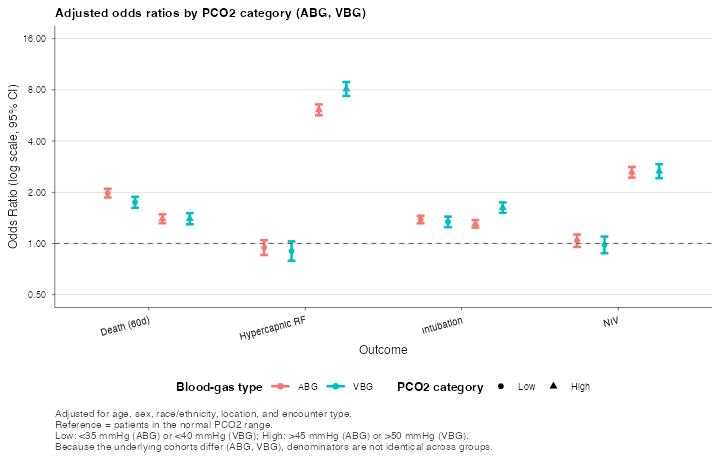
\includegraphics[width=0.94\linewidth,height=0.72\textheight,keepaspectratio]{Results/figs/or-plot-three-level-unweighted-report-preview.png}
\end{center}

\subsection{Observed outcome rates by CO2 bin
(unweighted)}\label{observed-outcome-rates-by-co2-bin-unweighted}

\begin{center}
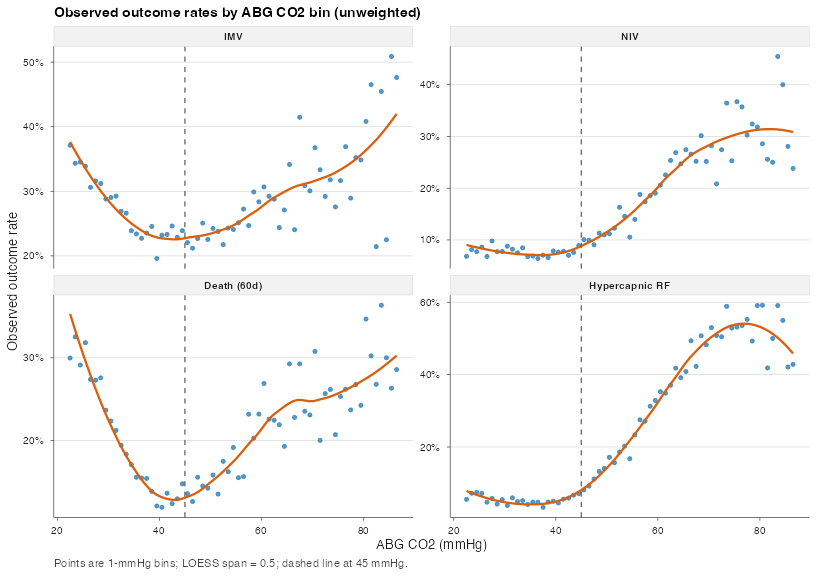
\includegraphics[width=0.94\linewidth,height=0.72\textheight,keepaspectratio]{Results/figs/co2-binned-rates-unweighted-abg-report-preview.png}
\end{center}

\begin{center}
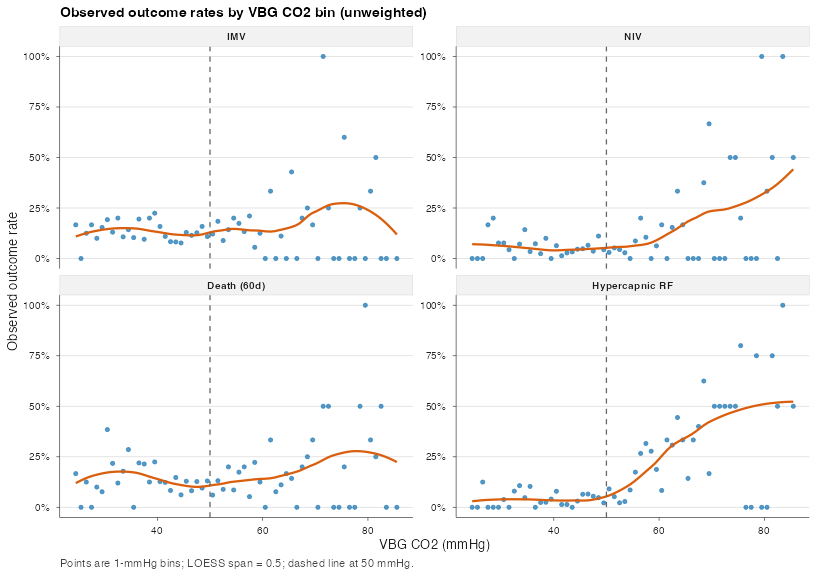
\includegraphics[width=0.94\linewidth,height=0.72\textheight,keepaspectratio]{Results/figs/co2-binned-rates-unweighted-vbg-report-preview.png}
\end{center}

\subsection{Restricted cubic spline regressions
(unweighted)}\label{restricted-cubic-spline-regressions-unweighted}

Spline curves are shown as odds ratios relative to CO2\_ref (midpoint of
the normal range), holding covariates at the reference profile.

\subsubsection{Unweighted, Restricted Cubic Spline Regression - ABG by
PaCO2}\label{unweighted-restricted-cubic-spline-regression---abg-by-paco2}

\subsubsection{Unweighted, Restricted Cubic Spline -
VBG}\label{unweighted-restricted-cubic-spline---vbg}

\begin{center}
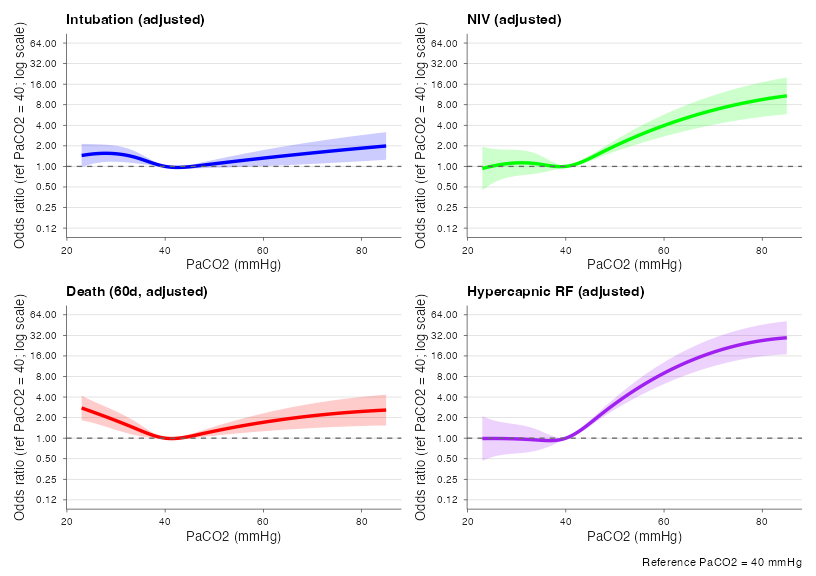
\includegraphics[width=0.94\linewidth,height=0.72\textheight,keepaspectratio]{Results/figs/spline-unweighted-abg-report-preview.png}
\end{center}

\begin{center}
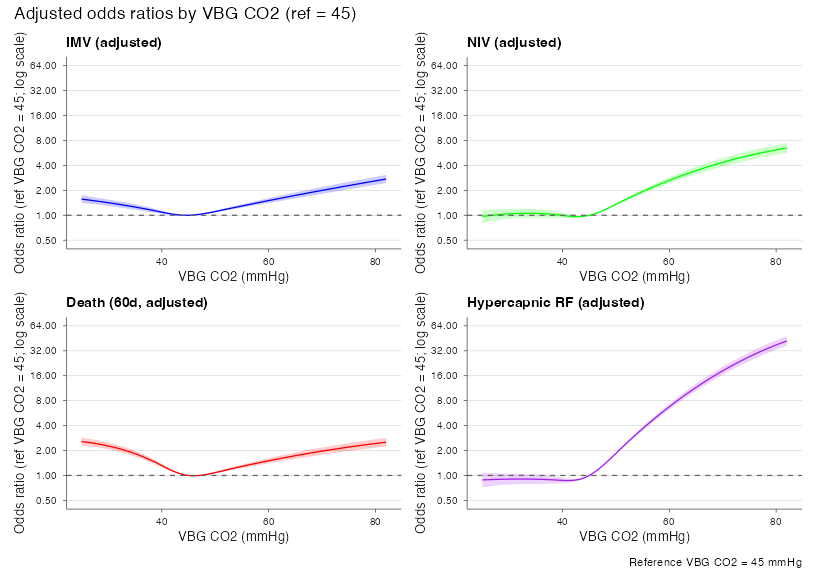
\includegraphics[width=0.94\linewidth,height=0.72\textheight,keepaspectratio]{Results/figs/spline-unweighted-vbg-report-preview.png}
\end{center}

\begin{center}
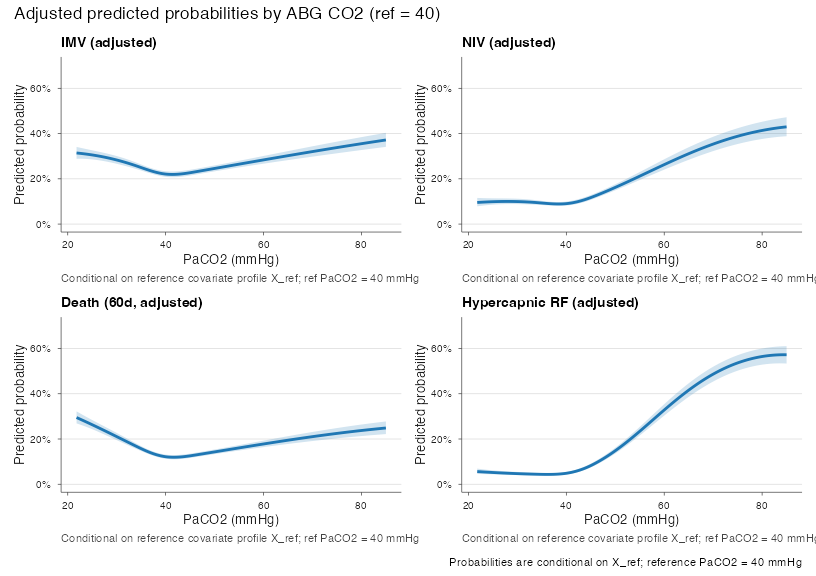
\includegraphics[width=0.94\linewidth,height=0.72\textheight,keepaspectratio]{Results/figs/spline-unweighted-abg-prob-report-preview.png}
\end{center}

\begin{center}
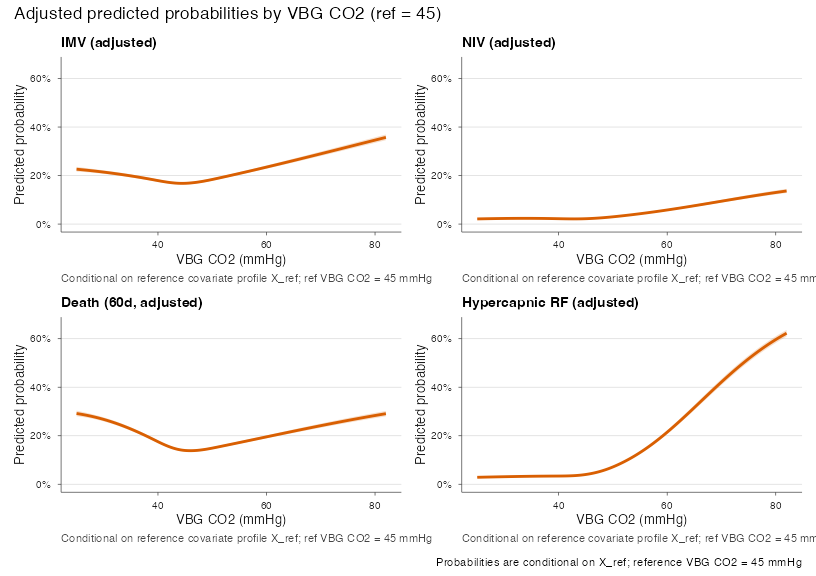
\includegraphics[width=0.94\linewidth,height=0.72\textheight,keepaspectratio]{Results/figs/spline-unweighted-vbg-prob-report-preview.png}
\end{center}

\FloatBarrier\nopagebreak

\par

\noindent

\section{Inverse Propensity Weighting
(GBM)}\label{inverse-propensity-weighting-gbm}

IPW done using Gradient Boosting Methods (GBM) - a type of decision-tree
based machine learning. ``\textbf{\emph{Random forests and GBM are
designed to automatically include relevant interactions for variables
included in the model.}} As such, using a GBM to estimate the PS model,
can reduce model misspecification, since \textbf{\emph{the analyst is
not required to identify relevant interactions or nonlinearities.''}}
from this citation: PMID:
\href{https://pubmed.ncbi.nlm.nih.gov/39947224/}{39947224}. PMCID:
\href{https://pmc.ncbi.nlm.nih.gov/articles/PMC11825193/}{PMC11825193}.

Current propensity score uses \texttt{covars\_gbm} (demographics,
comorbidities, encounter type, vitals, labs) as defined above; in this
block only \texttt{encounter\_type} is explicitly factored before
weighting.

Note: for all these, I suggested new GBM adjustments that accomplish the
following:

\begin{enumerate}
\def\labelenumi{\arabic{enumi}.}
\item
  Smaller GBM \& balance‑based stopping (stop.method = ``smd.max'') →
  faster fit, avoids over‑fitting, lighter tails (which lead to extreme
  weights that are problematic).
\item
  Target balance compares weighted treated cohort to the full sample;
  aim for \textbar SMD\textbar{} \textless{} 0.1.
\item
  Weight stabilization (divide by mean) mitigates a few huge weights. We
  use one‑sided truncation at very small propensities (caps large
  weights only).
\item
  Uses robust variance estimation (e.g.~allows the variances to change
  by PaCO2) for IP‑weighted GLM; works with splines via rcs(). This is a
  bit nuanced but I think good to change even though it adds complexity
\item
  Deterministic seed ensures result replication.
\end{enumerate}

\subsubsection{ABG IPW weighting and
diagnostics}\label{abg-ipw-weighting-and-diagnostics}

GBM tuning is shared across ABG and VBG via \texttt{gbm\_params} to keep
symmetry; update there if needed.

\textbf{Inverse Propensity-Weighted Logistic Regressions with CO2
predictor represented as a restricted cubic spline.}

These are covariate-adjusted outcome models (outcome \textasciitilde{}
spline(CO2) + X), fit separately for ABG and VBG cohorts using
survey::svyglm with robust (design-based) SEs. Spline curves are shown
as odds ratios relative to CO2\_ref (midpoint of the normal range).

\subsubsection{ABG IPW spline models}\label{abg-ipw-spline-models}

Restricting plots bewtween 0.02 and 0.98

\subsubsection{ABG IPW spline models (2--98th
percentile)}\label{abg-ipw-spline-models-298th-percentile}

\begin{center}
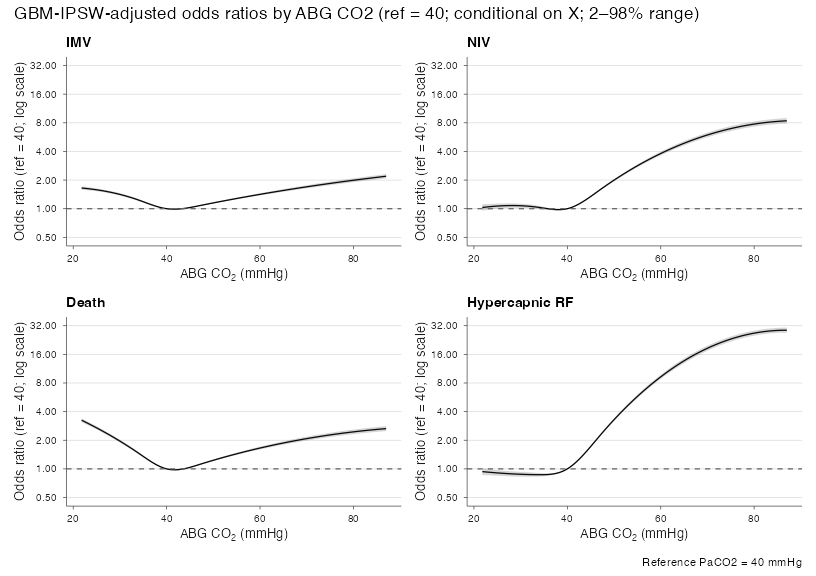
\includegraphics[width=0.94\linewidth,height=0.72\textheight,keepaspectratio]{Results/figs/spline-ipw-abg-trimmed-report-preview.png}
\end{center}

\begin{center}
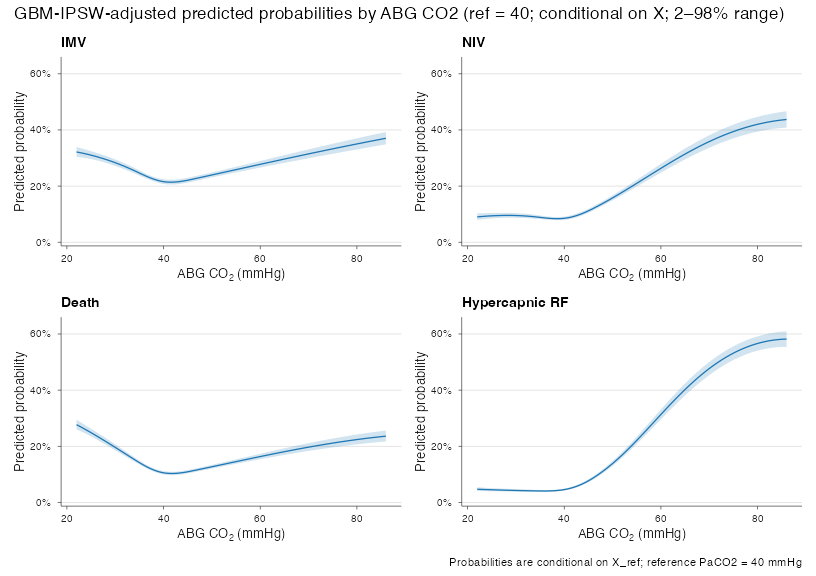
\includegraphics[width=0.94\linewidth,height=0.72\textheight,keepaspectratio]{Results/figs/spline-ipw-abg-trimmed-prob-report-preview.png}
\end{center}

VBG uses the same GBM tuning as ABG (shared \texttt{gbm\_params}).

\subsubsection{VBG IPW weighting and spline
models}\label{vbg-ipw-weighting-and-spline-models}

\begin{center}
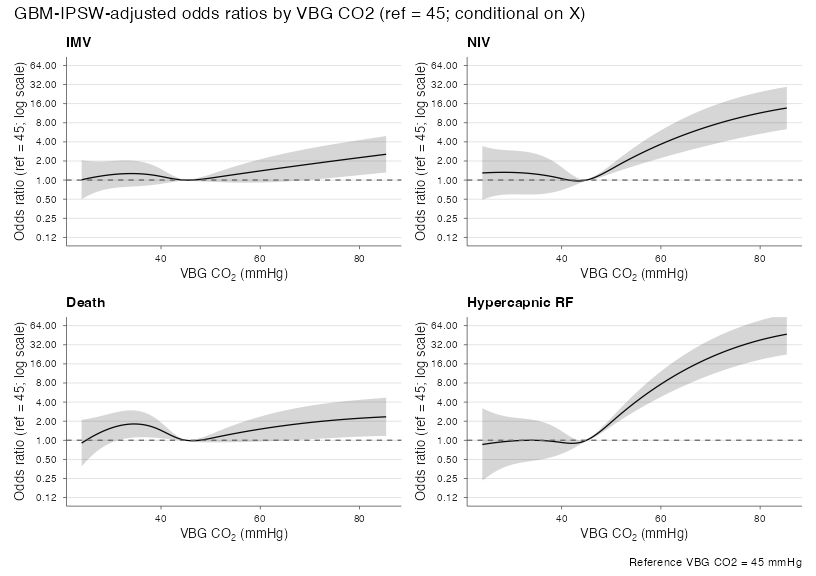
\includegraphics[width=0.94\linewidth,height=0.72\textheight,keepaspectratio]{Results/figs/spline-ipw-vbg-report-preview.png}
\end{center}

\begin{center}
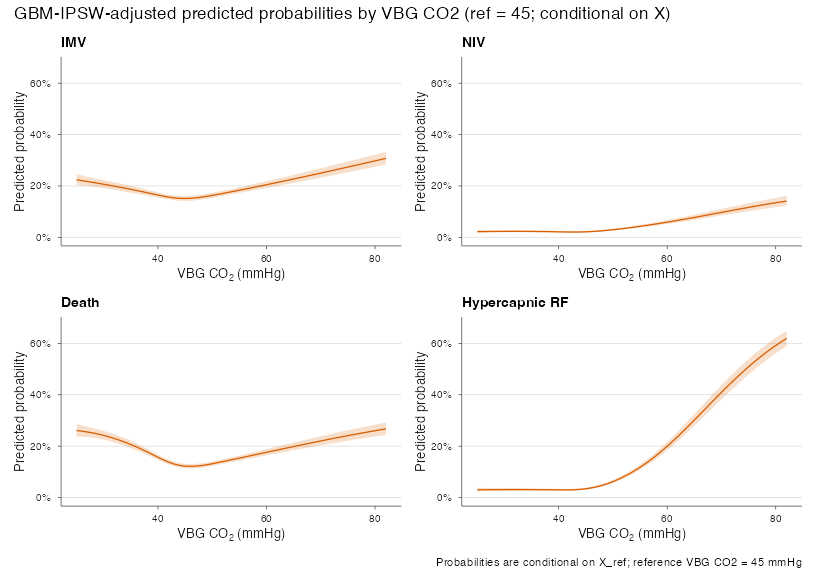
\includegraphics[width=0.94\linewidth,height=0.72\textheight,keepaspectratio]{Results/figs/spline-ipw-vbg-prob-report-preview.png}
\end{center}

\begin{center}
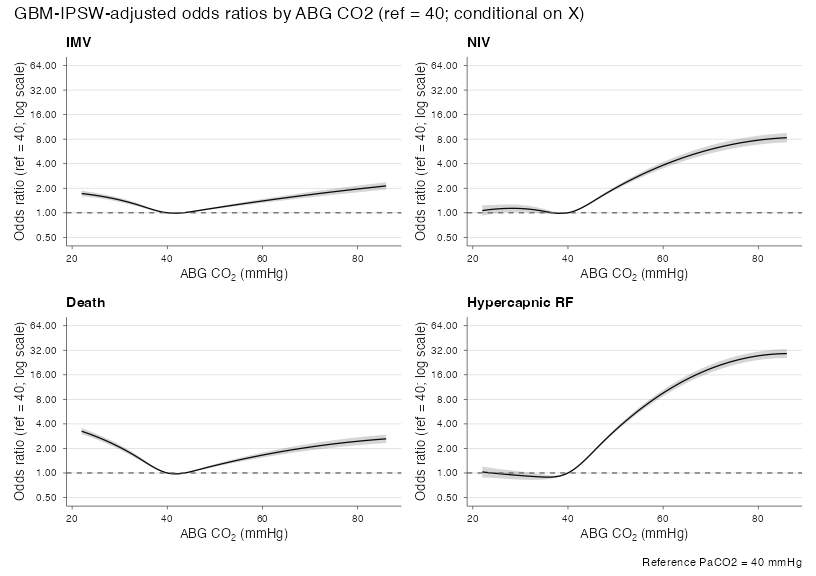
\includegraphics[width=0.94\linewidth,height=0.72\textheight,keepaspectratio]{Results/figs/spline-ipw-abg-shared-report-preview.png}
\end{center}

\begin{center}
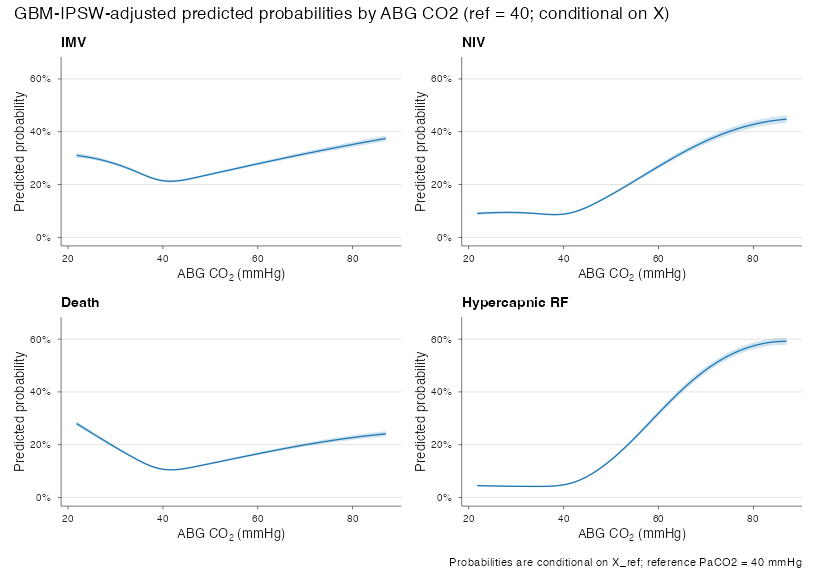
\includegraphics[width=0.94\linewidth,height=0.72\textheight,keepaspectratio]{Results/figs/spline-ipw-abg-shared-prob-report-preview.png}
\end{center}

\begin{center}
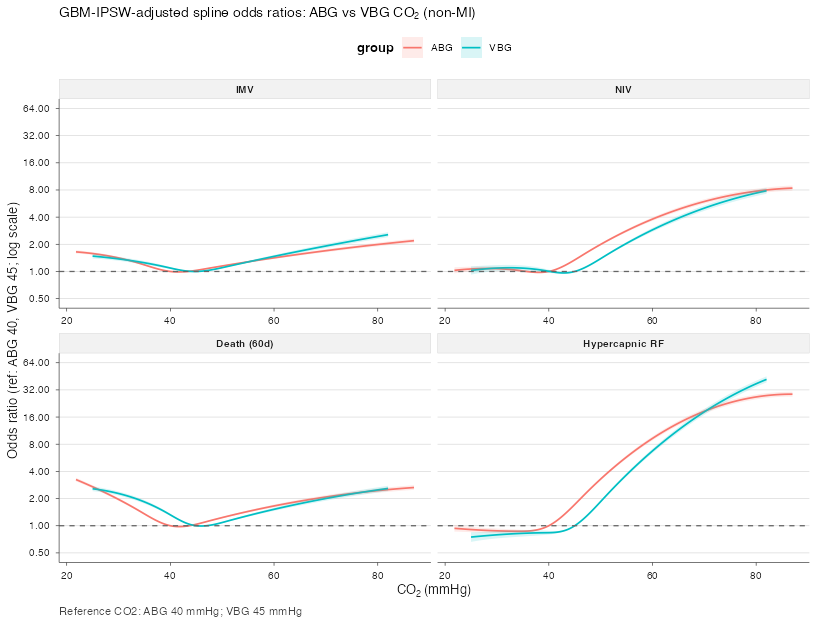
\includegraphics[width=0.94\linewidth,height=0.72\textheight,keepaspectratio]{Results/figs/spline-ipw-overlay-abg-vbg-report-preview.png}
\end{center}

\begin{center}
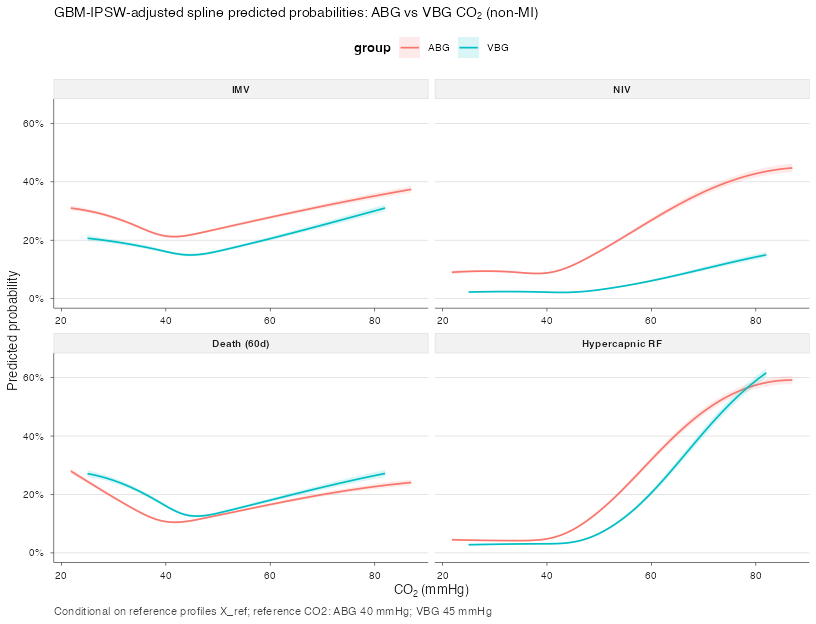
\includegraphics[width=0.94\linewidth,height=0.72\textheight,keepaspectratio]{Results/figs/spline-ipw-overlay-abg-vbg-prob-report-preview.png}
\end{center}

\subsubsection{Three-level PCO2 categories (weighted; ABG,
VBG)}\label{three-level-pco2-categories-weighted-abg-vbg}

Three groups with weights and covariate adjustment

\begin{center}
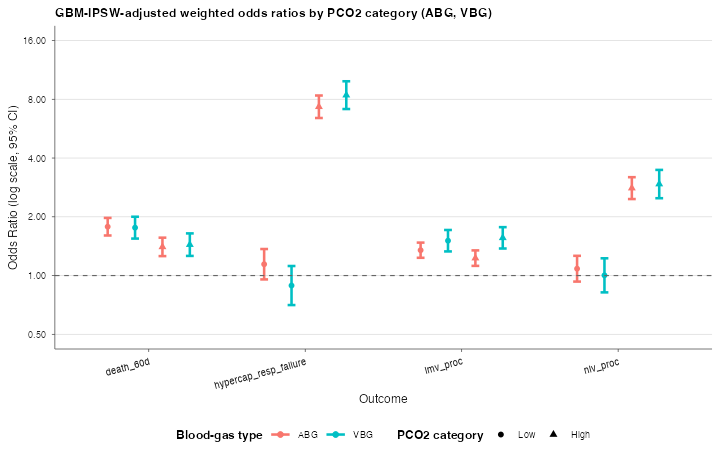
\includegraphics[width=0.94\linewidth,height=0.72\textheight,keepaspectratio]{Results/figs/or-plot-three-level-weighted-report-preview.png}
\end{center}

\subsubsection{Observed outcome rates by CO2 bin (GBM IPSW,
non-MI)}\label{observed-outcome-rates-by-co2-bin-gbm-ipsw-non-mi}

\begin{center}
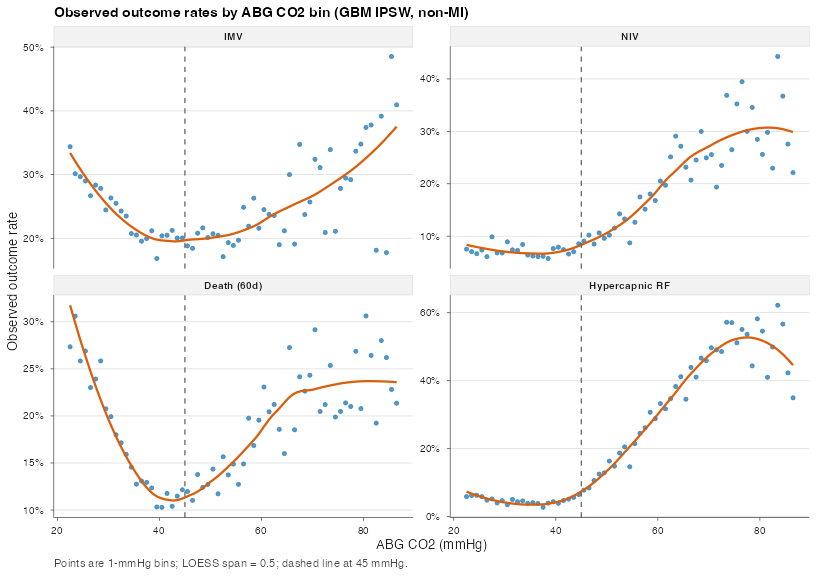
\includegraphics[width=0.94\linewidth,height=0.72\textheight,keepaspectratio]{Results/figs/co2-binned-rates-ipw-abg-report-preview.png}
\end{center}

\begin{center}
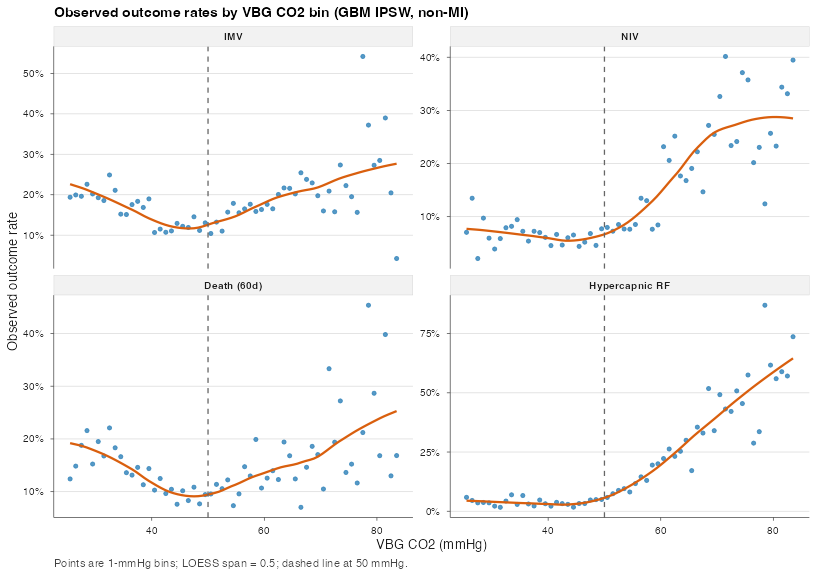
\includegraphics[width=0.94\linewidth,height=0.72\textheight,keepaspectratio]{Results/figs/co2-binned-rates-ipw-vbg-report-preview.png}
\end{center}

\subsection{Propensity score
diagnostics}\label{propensity-score-diagnostics}

Plotting propensity scores

\begin{center}
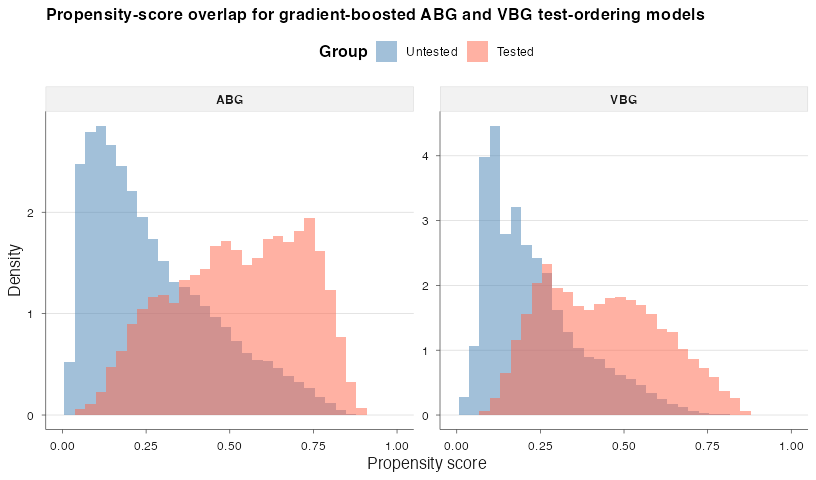
\includegraphics[width=0.94\linewidth,height=0.72\textheight,keepaspectratio]{Results/figs/propensity-histograms-conditional-report-preview.png}
\end{center}

\pandocbounded{
\includegraphics[keepaspectratio]{Results/figs/propensity-histograms-all-1.png}}

\begin{center}
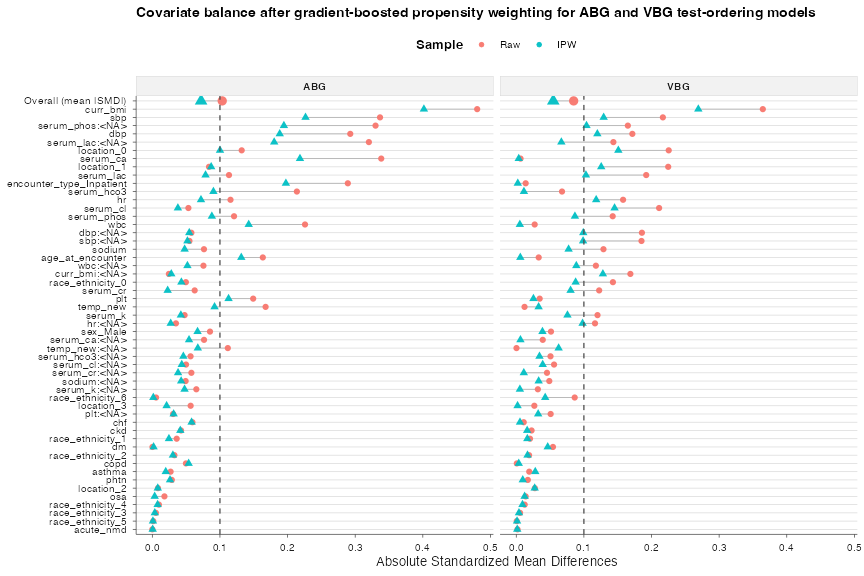
\includegraphics[width=0.94\linewidth,height=0.72\textheight,keepaspectratio]{Results/figs/loveplot-ipw-gbm-abg-vbg-report-preview.png}
\end{center}

\begin{center}
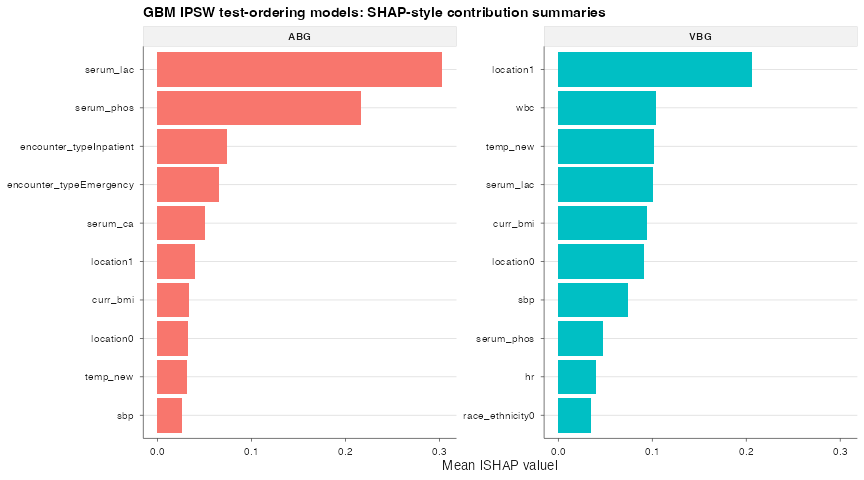
\includegraphics[width=0.94\linewidth,height=0.72\textheight,keepaspectratio]{Results/figs/shap-top10-ipw-gbm-abg-vbg-report-preview.png}
\end{center}

\section{Multiple Imputation (and logistic
IPSW)}\label{multiple-imputation-and-logistic-ipsw}

added 12/6/2025

\subsubsection{Missingness structure and
drivers}\label{missingness-structure-and-drivers}

\FloatBarrier\nopagebreak

\par

\noindent

\subsubsection{Monte Carlo error check after
MI}\label{monte-carlo-error-check-after-mi}

\subsection{Pre‑imputation data prep (consistent types \&
predictors)}\label{preimputation-data-prep-consistent-types-predictors}

\textbf{Why}: MI models need coherent types; using exactly the same
covariates as the propensity score models avoids model drift.

\subsection{Imputation model specification
(MICE)}\label{imputation-model-specification-mice}

\subsubsection{Predictor matrix \& methods. Run MICE (moderate settings
for
scale)}\label{predictor-matrix-methods.-run-mice-moderate-settings-for-scale}

\textbf{MC error diagnostic model:} Diagnostic model: imv\_proc
\textasciitilde{} has\_abg + age\_at\_encounter + curr\_bmi + sex +
encounter\_type (unweighted).

\begin{table}
\caption*{
{\fontsize{20}{25}\selectfont  Monte Carlo error vs SE (diagnostic only)\fontsize{12}{15}\selectfont }
} 
\fontsize{12.0pt}{14.0pt}\selectfont
\begin{tabular*}{\linewidth}{@{\extracolsep{\fill}}lrrrrrr}
\toprule
Term & Estimate & SE & MC error & MC error / SE & 2.5\% & 97.5\% \\ 
\midrule\addlinespace[2.5pt]
(Intercept) & -3.523 & 0.040 & 0.003 & 0.071 & -3.601523402 & -3.444523052 \\ 
has\_abg & 2.166 & 0.012 & 0.000 & 0.013 & 2.142966990 & 2.189596865 \\ 
age\_at\_encounter & -0.007 & 0.000 & 0.000 & 0.015 & -0.007546445 & -0.006429697 \\ 
curr\_bmi & -0.015 & 0.001 & 0.000 & 0.085 & -0.016798841 & -0.013049691 \\ 
sexMale & 0.285 & 0.010 & 0.000 & 0.013 & 0.265653428 & 0.303842195 \\ 
encounter\_typeInpatient & 1.125 & 0.015 & 0.000 & 0.004 & 1.094833080 & 1.155174813 \\ 
\bottomrule
\end{tabular*}
\end{table}

\pandocbounded{
\includegraphics[keepaspectratio]{Results/figs/mi-diagnostics-1.png}}

\pandocbounded{
\includegraphics[keepaspectratio]{Results/figs/mi-diagnostics-2.png}}

\pandocbounded{
\includegraphics[keepaspectratio]{Results/figs/mi-diagnostics-3.png}}

\pandocbounded{
\includegraphics[keepaspectratio]{Results/figs/mi-imputation-diagnostics-1.png}}

\pandocbounded{
\includegraphics[keepaspectratio]{Results/figs/mi-imputation-diagnostics-2.png}}

\pandocbounded{
\includegraphics[keepaspectratio]{Results/figs/mi-imputation-diagnostics-3.png}}

\pandocbounded{
\includegraphics[keepaspectratio]{Results/figs/mi-imputation-diagnostics-4.png}}

\pandocbounded{
\includegraphics[keepaspectratio]{Results/figs/mi-imputation-diagnostics-5.png}}

\pandocbounded{
\includegraphics[keepaspectratio]{Results/figs/mi-imputation-diagnostics-6.png}}

\pandocbounded{
\includegraphics[keepaspectratio]{Results/figs/mi-imputation-diagnostics-7.png}}

\pandocbounded{
\includegraphics[keepaspectratio]{Results/figs/mi-imputation-diagnostics-8.png}}

\pandocbounded{
\includegraphics[keepaspectratio]{Results/figs/mi-imputation-diagnostics-9.png}}

\pandocbounded{
\includegraphics[keepaspectratio]{Results/figs/mi-imputation-diagnostics-10.png}}

\pandocbounded{
\includegraphics[keepaspectratio]{Results/figs/mi-imputation-diagnostics-11.png}}

\pandocbounded{
\includegraphics[keepaspectratio]{Results/figs/mi-imputation-diagnostics-12.png}}

\pandocbounded{
\includegraphics[keepaspectratio]{Results/figs/mi-imputation-diagnostics-13.png}}

\pandocbounded{
\includegraphics[keepaspectratio]{Results/figs/mi-imputation-diagnostics-14.png}}

\pandocbounded{
\includegraphics[keepaspectratio]{Results/figs/mi-imputation-diagnostics-15.png}}

\pandocbounded{
\includegraphics[keepaspectratio]{Results/figs/mi-imputation-diagnostics-16.png}}

\pandocbounded{
\includegraphics[keepaspectratio]{Results/figs/mi-imputation-diagnostics-17.png}}

\pandocbounded{
\includegraphics[keepaspectratio]{Results/figs/mi-imputation-diagnostics-18.png}}

\pandocbounded{
\includegraphics[keepaspectratio]{Results/figs/mi-imputation-diagnostics-19.png}}

\pandocbounded{
\includegraphics[keepaspectratio]{Results/figs/mi-imputation-diagnostics-20.png}}

\pandocbounded{
\includegraphics[keepaspectratio]{Results/figs/mi-imputation-diagnostics-21.png}}

\pandocbounded{
\includegraphics[keepaspectratio]{Results/figs/mi-imputation-diagnostics-22.png}}

\pandocbounded{
\includegraphics[keepaspectratio]{Results/figs/mi-imputation-diagnostics-23.png}}

\pandocbounded{
\includegraphics[keepaspectratio]{Results/figs/mi-imputation-diagnostics-24.png}}

\pandocbounded{
\includegraphics[keepaspectratio]{Results/figs/mi-imputation-diagnostics-25.png}}

\pandocbounded{
\includegraphics[keepaspectratio]{Results/figs/mi-imputation-diagnostics-26.png}}

\pandocbounded{
\includegraphics[keepaspectratio]{Results/figs/mi-imputation-diagnostics-27.png}}

\pandocbounded{
\includegraphics[keepaspectratio]{Results/figs/mi-imputation-diagnostics-28.png}}

\pandocbounded{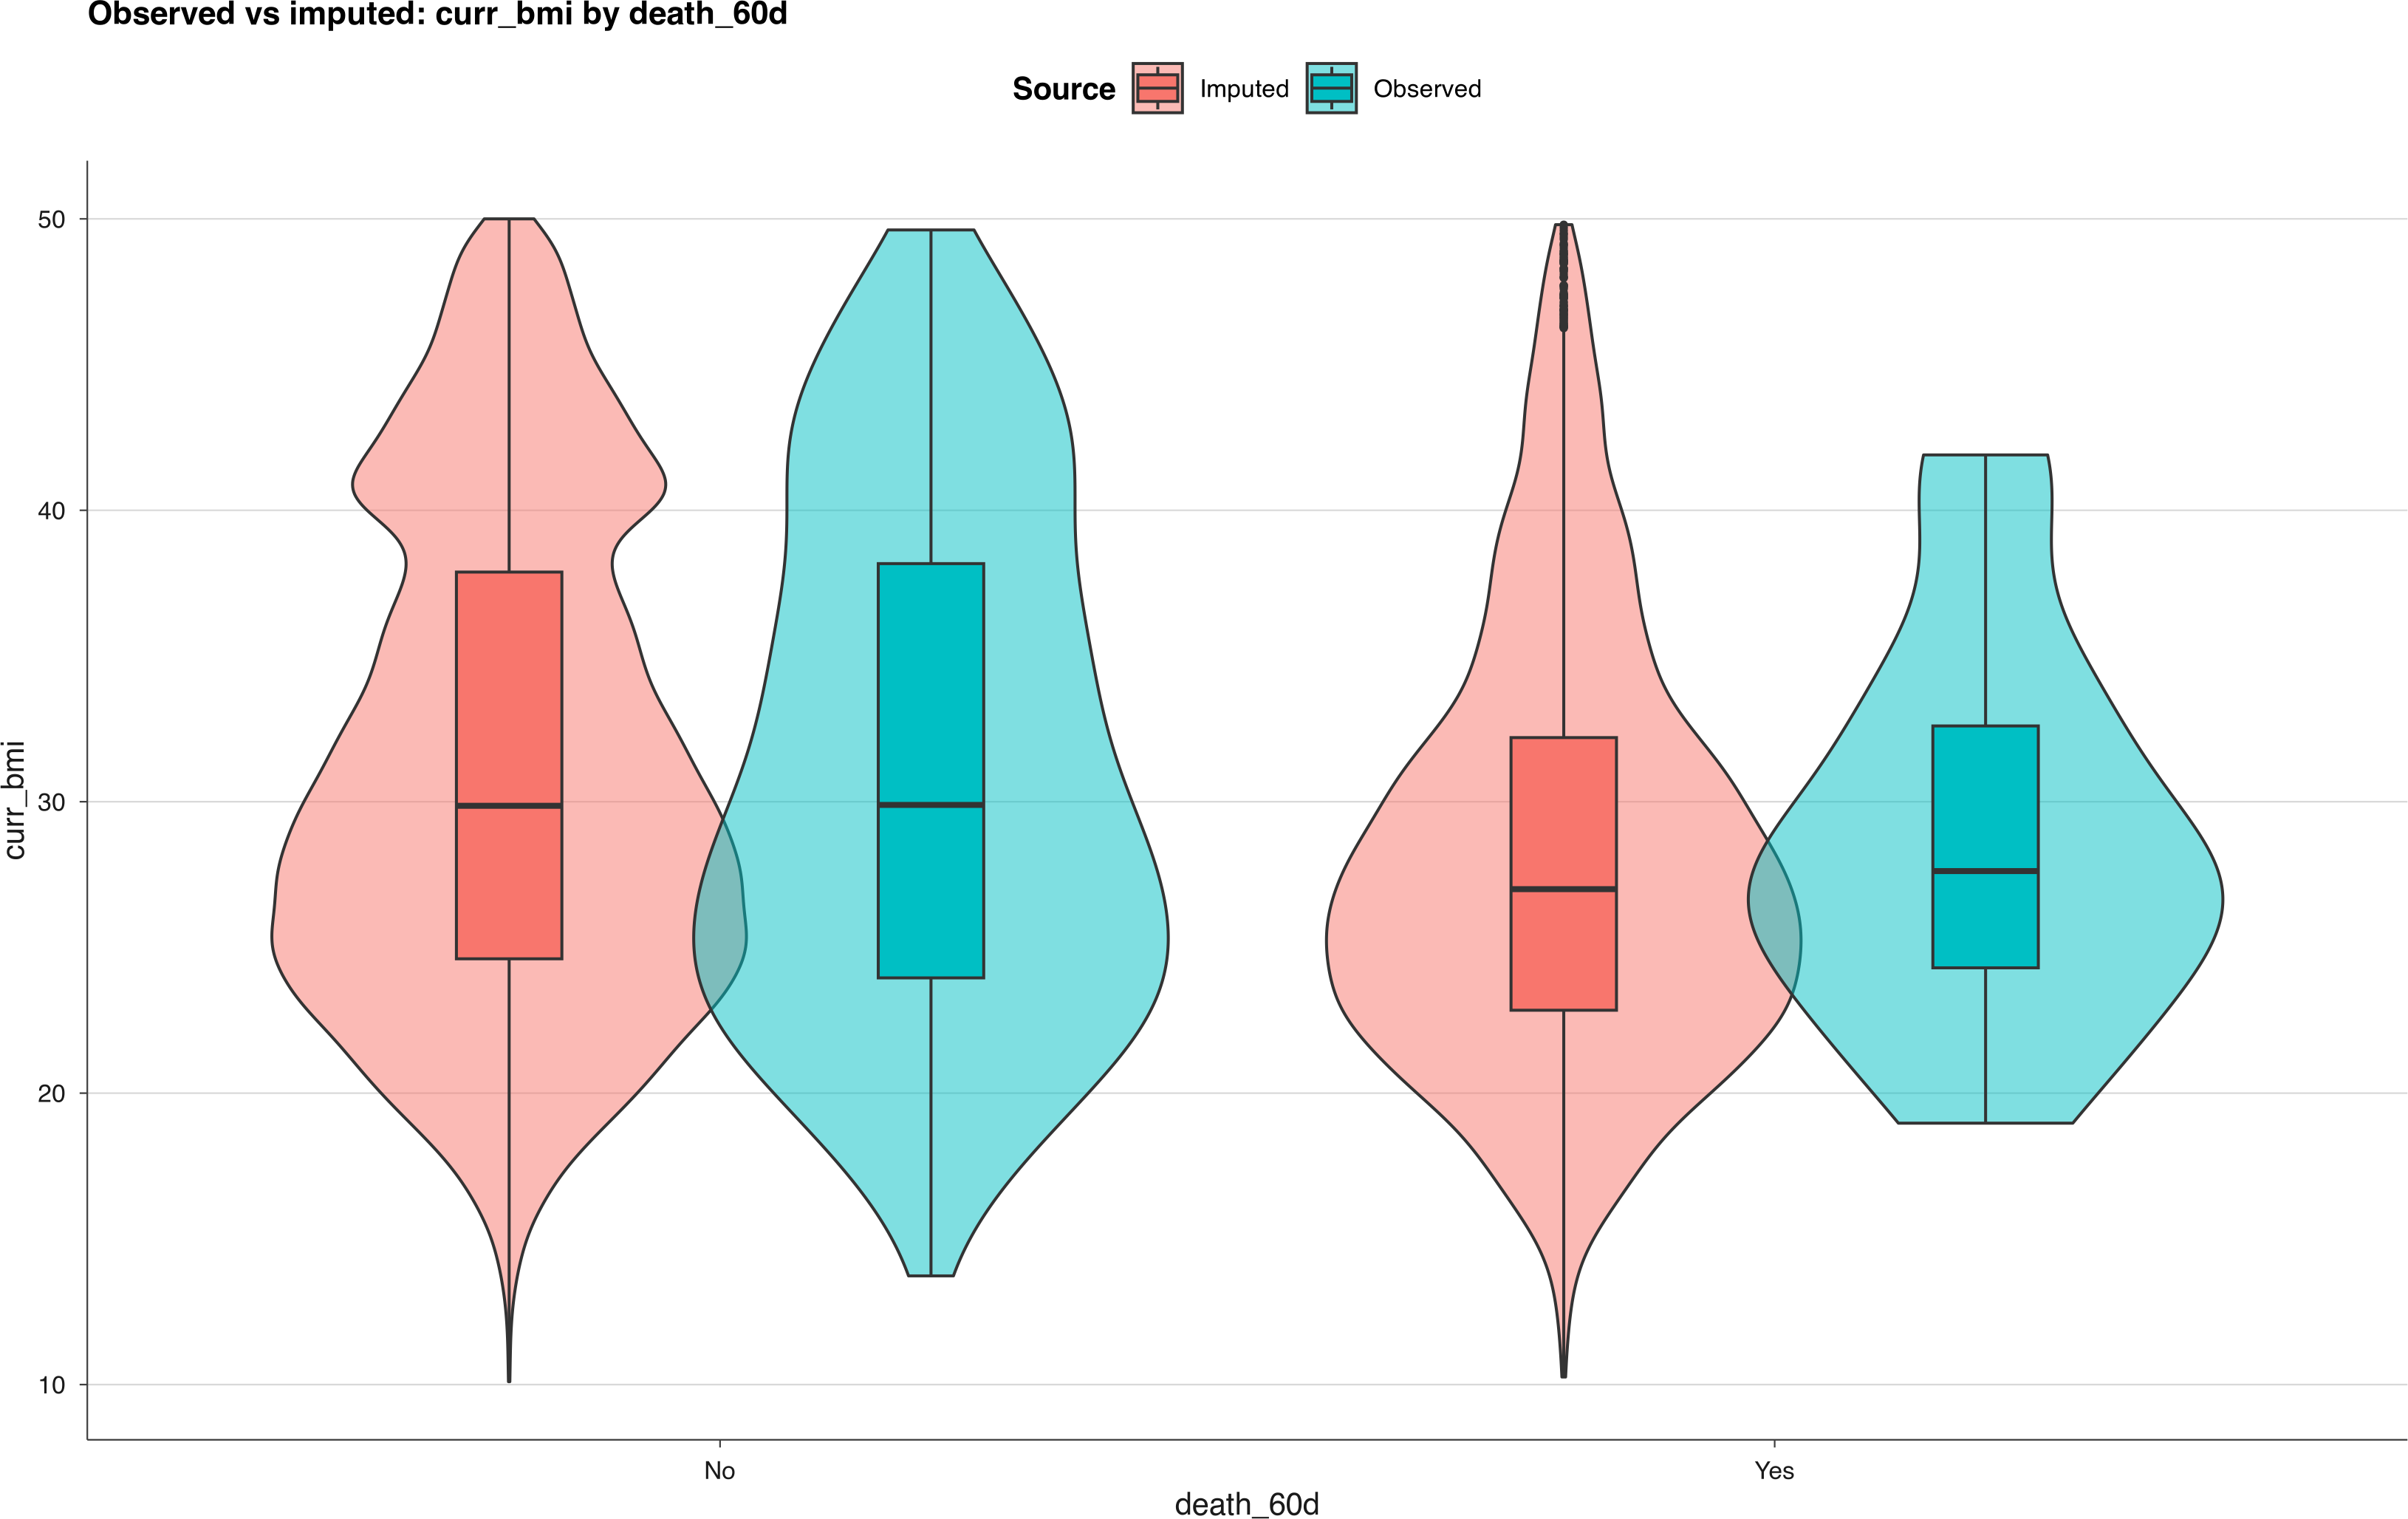
\includegraphics[keepaspectratio]{Results/figs/mi-imputation-diagnostics-29.png}}

\pandocbounded{
\includegraphics[keepaspectratio]{Results/figs/mi-imputation-diagnostics-30.png}}

\pandocbounded{
\includegraphics[keepaspectratio]{Results/figs/mi-missing-audit-1.png}}

\pandocbounded{
\includegraphics[keepaspectratio]{Results/figs/mi-missing-audit-2.png}}

\subsection{Refit propensity models within each
imputation}\label{refit-propensity-models-within-each-imputation}

MI propensity scores use logistic regression with restricted cubic
splines (\texttt{rms::rcs}, 4 knots by default) for continuous
covariates; the same covariate set used in non‑MI models is reused here
(\texttt{covars\_ps}). IPSW truncation rules are unchanged.

Note: the MI computations below run in a single pass per imputation
(weights, balance, cat3, spline). Subsequent MI sections reuse those
outputs and will stop if they are missing.

\subsubsection{FAIL-FAST CHECKS}\label{fail-fast-checks}

\begin{verbatim}
             used    (Mb) gc trigger    (Mb) limit (Mb)   max used    (Mb)
Ncells    7584270   405.1   13521818   722.2         NA   13521818   722.2
Vcells 1539815247 11747.9 2147380309 16383.3      16384 2147378644 16383.2
\end{verbatim}

\subsubsection{ABG propensity (has\_abg)}\label{abg-propensity-has_abg}

\subsubsection{Balance diagnostics across
imputations}\label{balance-diagnostics-across-imputations}

\subsubsection{VBG propensity (has\_vbg)}\label{vbg-propensity-has_vbg}

\subsubsection{VBG balance}\label{vbg-balance}

\subsection{Weighted outcome models within each imputation +
pooling}\label{weighted-outcome-models-within-each-imputation-pooling}

Within each imputation, fit covariate‑adjusted CO2 spline outcome models
\textbf{only in the measured cohort} (has\_abg==1 for PaCO2; has\_vbg==1
for VBG CO2), using IPSW weights to address nonrandom testing. Curves
are pooled pointwise across imputations (Rubin's rules on the log‑OR
scale) and displayed as odds ratios relative to CO2\_ref at a reference
covariate profile.

\subsubsection{Helper: fit + extract log‑OR and SE from
svyglm}\label{helper-fit-extract-logor-and-se-from-svyglm}

\subsubsection{VBG: MI pooled spline models (treated cohort
only)}\label{vbg-mi-pooled-spline-models-treated-cohort-only}

\subsection{Explainability}\label{explainability}

\subsection{MI three‑level PCO2 helpers and
checks}\label{mi-threelevel-pco2-helpers-and-checks}

\subsection{MI + IPW three-level PCO2 (ABG \&
VBG)}\label{mi-ipw-three-level-pco2-abg-vbg}

\subsubsection{ABG: MI + IPW, three-level PCO2
outcomes}\label{abg-mi-ipw-three-level-pco2-outcomes}

\subsubsection{VBG: MI + IPW, three-level PCO2
outcomes}\label{vbg-mi-ipw-three-level-pco2-outcomes}

\subsubsection{MI-pooled IPW associations (3-level
CO2)}\label{mi-pooled-ipw-associations-3-level-co2}

\begin{table}
\caption*{
{\fontsize{20}{25}\selectfont  MI-pooled MI-logistic IPSW associations between CO2 category and outcomes (adjusted)\fontsize{12}{15}\selectfont }
} 
\fontsize{12.0pt}{14.0pt}\selectfont
\begin{tabular*}{\linewidth}{@{\extracolsep{\fill}}llrr}
\toprule
Cohort & Outcome & Low vs normal OR (95\% CI) & High vs normal OR (95\% CI) \\ 
\midrule\addlinespace[2.5pt]
ABG & IMV & 1.34 (1.30, 1.38) & 1.33 (1.29, 1.37) \\ 
ABG & NIV & 0.99 (0.95, 1.05) & 2.64 (2.53, 2.75) \\ 
ABG & Death (60d) & 1.89 (1.83, 1.96) & 1.40 (1.35, 1.45) \\ 
ABG & Hypercapnic RF & 0.92 (0.87, 0.98) & 6.23 (5.97, 6.50) \\ 
VBG & IMV & 1.31 (1.25, 1.36) & 1.54 (1.48, 1.61) \\ 
VBG & NIV & 1.01 (0.94, 1.08) & 2.93 (2.77, 3.10) \\ 
VBG & Death (60d) & 1.79 (1.71, 1.87) & 1.42 (1.35, 1.48) \\ 
VBG & Hypercapnic RF & 0.84 (0.77, 0.91) & 8.00 (7.55, 8.47) \\ 
\bottomrule
\end{tabular*}
\begin{minipage}{\linewidth}
\vspace{.05em}
Weighted survey GLMs adjusted for baseline covariates; weights = MI-specific GLM (RCS) IPW; m = 80 imputations (seed 20251206); reference = Normal.\\
\end{minipage}
\end{table}

\subsubsection{Summary: adjusted CO2-category associations across
analysis
tracks}\label{summary-adjusted-co2-category-associations-across-analysis-tracks}

\begin{landscape}

\begin{center}\textbf{Categorical key results for the ABG cohort across crude, unweighted adjusted, imputed non-weighted, MI-logistic IPSW-weighted, and GBM IPSW-weighted analyses; probabilities are conditional on X\_ref except in the crude track.}\end{center}

\begin{table}[!h]
\centering\begingroup\fontsize{6}{8}\selectfont

\resizebox{\ifdim\width>\linewidth\linewidth\else\width\fi}{!}{
\begin{tabular}{rrllll}
\toprule
n\_model & events & method & group & outcome & Low vs normal OR (95\% CI)\\
\midrule
187242 & 48173 & Crude & ABG & IMV & 1.34 (1.31, 1.38)\\
187242 & 19040 & Crude & ABG & NIV & 1.01 (0.97, 1.05)\\
187242 & 32718 & Crude & ABG & Death (60d) & 1.90 (1.85, 1.95)\\
187242 & 20276 & Crude & ABG & Hypercapnic RF & 0.92 (0.87, 0.97)\\
187242 & 48173 & Adjusted & ABG & IMV & 1.36 (1.33, 1.39)\\
\addlinespace
187242 & 19040 & Adjusted & ABG & NIV & 1.00 (0.96, 1.04)\\
187242 & 32718 & Adjusted & ABG & Death (60d) & 1.98 (1.92, 2.04)\\
187242 & 20276 & Adjusted & ABG & Hypercapnic RF & 0.91 (0.87, 0.96)\\
187242 & 48173 & Imputed & ABG & IMV & 1.36 (1.33, 1.39)\\
187242 & 19040 & Imputed & ABG & NIV & 1.00 (0.96, 1.04)\\
\addlinespace
187242 & 32718 & Imputed & ABG & Death (60d) & 1.98 (1.92, 2.04)\\
187242 & 20276 & Imputed & ABG & Hypercapnic RF & 0.91 (0.87, 0.96)\\
187242 & 48173 & Weighted and adjusted & ABG & IMV & 1.34 (1.30, 1.38)\\
187242 & 19040 & Weighted and adjusted & ABG & NIV & 0.99 (0.95, 1.05)\\
187242 & 32718 & Weighted and adjusted & ABG & Death (60d) & 1.89 (1.83, 1.96)\\
\addlinespace
187242 & 20276 & Weighted and adjusted & ABG & Hypercapnic RF & 0.92 (0.87, 0.98)\\
187242 & 48173 & GBM-weighted & ABG & IMV & 1.36 (1.32, 1.40)\\
187242 & 19040 & GBM-weighted & ABG & NIV & 0.99 (0.95, 1.04)\\
187242 & 32718 & GBM-weighted & ABG & Death (60d) & 1.93 (1.87, 2.00)\\
187242 & 20276 & GBM-weighted & ABG & Hypercapnic RF & 0.94 (0.89, 0.99)\\
\bottomrule
\end{tabular}}
\endgroup{}
\end{table}

\begin{table}[!h]
\centering\begingroup\fontsize{6}{8}\selectfont

\resizebox{\ifdim\width>\linewidth\linewidth\else\width\fi}{!}{
\begin{tabular}{llll}
\toprule
High vs normal OR (95\% CI) & Normal probability (95\% CI) & Low probability (95\% CI) & High probability (95\% CI)\\
\midrule
1.24 (1.21, 1.27) & 0.23 (0.23, 0.23) & 0.29 (0.28, 0.29) & 0.27 (0.27, 0.28)\\
2.42 (2.34, 2.50) & 0.08 (0.07, 0.08) & 0.08 (0.07, 0.08) & 0.17 (0.16, 0.17)\\
1.47 (1.42, 1.51) & 0.14 (0.13, 0.14) & 0.23 (0.23, 0.23) & 0.19 (0.18, 0.19)\\
5.82 (5.62, 6.03) & 0.05 (0.05, 0.06) & 0.05 (0.05, 0.05) & 0.25 (0.25, 0.25)\\
1.31 (1.28, 1.34) & 0.23 (0.22, 0.23) & 0.29 (0.28, 0.29) & 0.28 (0.27, 0.28)\\
\addlinespace
2.65 (2.56, 2.74) & 0.10 (0.09, 0.10) & 0.10 (0.09, 0.10) & 0.22 (0.21, 0.23)\\
1.43 (1.38, 1.47) & 0.13 (0.13, 0.13) & 0.23 (0.22, 0.23) & 0.17 (0.17, 0.18)\\
6.04 (5.83, 6.26) & 0.05 (0.05, 0.05) & 0.05 (0.05, 0.05) & 0.25 (0.25, 0.26)\\
1.31 (1.28, 1.34) & 0.23 (0.22, 0.23) & 0.29 (0.28, 0.29) & 0.28 (0.27, 0.28)\\
2.65 (2.56, 2.74) & 0.10 (0.09, 0.10) & 0.10 (0.09, 0.10) & 0.22 (0.22, 0.23)\\
\addlinespace
1.43 (1.38, 1.47) & 0.13 (0.13, 0.13) & 0.23 (0.22, 0.23) & 0.17 (0.17, 0.18)\\
6.04 (5.82, 6.26) & 0.05 (0.05, 0.05) & 0.05 (0.05, 0.05) & 0.25 (0.25, 0.26)\\
1.33 (1.29, 1.37) & 0.21 (0.20, 0.21) & 0.26 (0.25, 0.26) & 0.26 (0.25, 0.26)\\
2.64 (2.53, 2.75) & 0.09 (0.09, 0.09) & 0.09 (0.08, 0.09) & 0.21 (0.20, 0.21)\\
1.40 (1.35, 1.45) & 0.11 (0.11, 0.11) & 0.19 (0.19, 0.20) & 0.15 (0.14, 0.15)\\
\addlinespace
6.23 (5.97, 6.50) & 0.04 (0.04, 0.05) & 0.04 (0.04, 0.04) & 0.22 (0.22, 0.23)\\
1.30 (1.26, 1.33) & 0.22 (0.22, 0.22) & 0.28 (0.27, 0.28) & 0.27 (0.26, 0.27)\\
2.68 (2.57, 2.79) & 0.09 (0.09, 0.10) & 0.09 (0.09, 0.10) & 0.21 (0.21, 0.22)\\
1.45 (1.40, 1.50) & 0.11 (0.11, 0.11) & 0.20 (0.19, 0.20) & 0.15 (0.15, 0.16)\\
6.59 (6.33, 6.86) & 0.05 (0.04, 0.05) & 0.04 (0.04, 0.04) & 0.24 (0.23, 0.24)\\
\bottomrule
\end{tabular}}
\endgroup{}
\end{table}

\end{landscape}

\begin{landscape}

\begin{center}\textbf{Categorical key results for the VBG cohort across crude, unweighted adjusted, imputed non-weighted, MI-logistic IPSW-weighted, and GBM IPSW-weighted analyses; probabilities are conditional on X\_ref except in the crude track.}\end{center}

\begin{table}[!h]
\centering\begingroup\fontsize{6}{8}\selectfont

\resizebox{\ifdim\width>\linewidth\linewidth\else\width\fi}{!}{
\begin{tabular}{rrllll}
\toprule
n\_model & events & method & group & outcome & Low vs normal OR (95\% CI)\\
\midrule
149663 & 23217 & Crude & VBG & IMV & 1.48 (1.43, 1.54)\\
149663 & 10699 & Crude & VBG & NIV & 1.18 (1.12, 1.25)\\
149663 & 20483 & Crude & VBG & Death (60d) & 1.78 (1.71, 1.84)\\
149663 & 13228 & Crude & VBG & Hypercapnic RF & 0.98 (0.92, 1.04)\\
149663 & 23217 & Adjusted & VBG & IMV & 1.28 (1.24, 1.33)\\
\addlinespace
149663 & 10699 & Adjusted & VBG & NIV & 1.00 (0.94, 1.06)\\
149663 & 20483 & Adjusted & VBG & Death (60d) & 1.78 (1.72, 1.85)\\
149663 & 13228 & Adjusted & VBG & Hypercapnic RF & 0.82 (0.77, 0.88)\\
149663 & 23217 & Imputed & VBG & IMV & 1.28 (1.24, 1.33)\\
149663 & 10699 & Imputed & VBG & NIV & 1.00 (0.94, 1.06)\\
\addlinespace
149663 & 20483 & Imputed & VBG & Death (60d) & 1.78 (1.72, 1.85)\\
149663 & 13228 & Imputed & VBG & Hypercapnic RF & 0.82 (0.77, 0.88)\\
149663 & 23217 & Weighted and adjusted & VBG & IMV & 1.31 (1.25, 1.36)\\
149663 & 10699 & Weighted and adjusted & VBG & NIV & 1.01 (0.94, 1.08)\\
149663 & 20483 & Weighted and adjusted & VBG & Death (60d) & 1.79 (1.71, 1.87)\\
\addlinespace
149663 & 13228 & Weighted and adjusted & VBG & Hypercapnic RF & 0.84 (0.77, 0.91)\\
149663 & 23217 & GBM-weighted & VBG & IMV & 1.31 (1.25, 1.36)\\
149663 & 10699 & GBM-weighted & VBG & NIV & 1.01 (0.95, 1.08)\\
149663 & 20483 & GBM-weighted & VBG & Death (60d) & 1.77 (1.70, 1.85)\\
149663 & 13228 & GBM-weighted & VBG & Hypercapnic RF & 0.86 (0.80, 0.93)\\
\bottomrule
\end{tabular}}
\endgroup{}
\end{table}

\begin{table}[!h]
\centering\begingroup\fontsize{6}{8}\selectfont

\resizebox{\ifdim\width>\linewidth\linewidth\else\width\fi}{!}{
\begin{tabular}{llll}
\toprule
High vs normal OR (95\% CI) & Normal probability (95\% CI) & Low probability (95\% CI) & High probability (95\% CI)\\
\midrule
1.67 (1.61, 1.73) & 0.12 (0.12, 0.13) & 0.17 (0.17, 0.18) & 0.19 (0.19, 0.19)\\
2.89 (2.76, 3.03) & 0.05 (0.05, 0.05) & 0.06 (0.05, 0.06) & 0.13 (0.12, 0.13)\\
1.61 (1.55, 1.67) & 0.10 (0.10, 0.11) & 0.17 (0.17, 0.18) & 0.16 (0.15, 0.16)\\
7.67 (7.33, 8.03) & 0.04 (0.04, 0.04) & 0.04 (0.03, 0.04) & 0.23 (0.23, 0.23)\\
1.60 (1.55, 1.66) & 0.17 (0.16, 0.17) & 0.21 (0.20, 0.21) & 0.25 (0.24, 0.25)\\
\addlinespace
2.80 (2.67, 2.94) & 0.02 (0.02, 0.02) & 0.02 (0.02, 0.02) & 0.06 (0.06, 0.07)\\
1.44 (1.39, 1.49) & 0.15 (0.14, 0.15) & 0.24 (0.23, 0.24) & 0.20 (0.19, 0.21)\\
7.70 (7.35, 8.07) & 0.04 (0.04, 0.04) & 0.03 (0.03, 0.04) & 0.25 (0.24, 0.25)\\
1.60 (1.55, 1.66) & 0.17 (0.16, 0.17) & 0.21 (0.20, 0.21) & 0.25 (0.24, 0.25)\\
2.80 (2.67, 2.94) & 0.02 (0.02, 0.02) & 0.02 (0.02, 0.03) & 0.06 (0.06, 0.07)\\
\addlinespace
1.44 (1.39, 1.49) & 0.15 (0.14, 0.15) & 0.24 (0.23, 0.24) & 0.20 (0.19, 0.21)\\
7.70 (7.35, 8.07) & 0.04 (0.04, 0.04) & 0.03 (0.03, 0.04) & 0.25 (0.24, 0.25)\\
1.54 (1.48, 1.61) & 0.17 (0.16, 0.17) & 0.21 (0.20, 0.21) & 0.23 (0.23, 0.24)\\
2.93 (2.77, 3.10) & 0.02 (0.02, 0.02) & 0.02 (0.02, 0.02) & 0.06 (0.06, 0.07)\\
1.42 (1.35, 1.48) & 0.13 (0.12, 0.13) & 0.21 (0.20, 0.21) & 0.17 (0.16, 0.18)\\
\addlinespace
8.00 (7.55, 8.47) & 0.04 (0.03, 0.04) & 0.03 (0.03, 0.03) & 0.23 (0.22, 0.24)\\
1.55 (1.49, 1.61) & 0.15 (0.15, 0.16) & 0.19 (0.18, 0.19) & 0.21 (0.21, 0.22)\\
2.91 (2.76, 3.06) & 0.02 (0.02, 0.03) & 0.02 (0.02, 0.03) & 0.07 (0.06, 0.07)\\
1.46 (1.40, 1.52) & 0.13 (0.13, 0.14) & 0.22 (0.21, 0.22) & 0.18 (0.18, 0.19)\\
8.21 (7.79, 8.65) & 0.04 (0.03, 0.04) & 0.03 (0.03, 0.03) & 0.24 (0.23, 0.24)\\
\bottomrule
\end{tabular}}
\endgroup{}
\end{table}

\end{landscape}

\begin{landscape}

\begin{center}\textbf{Adjusted odds ratios (low/high vs normal) across unweighted adjusted, GBM IPSW-weighted, and MI-logistic IPSW-weighted analysis tracks for the ABG cohort; n/events reflect model sample size (median across imputations for MI-based tracks).}\end{center}

\begin{table}[!h]
\centering\begingroup\fontsize{7}{9}\selectfont

\resizebox{\ifdim\width>\linewidth\linewidth\else\width\fi}{!}{
\begin{tabular}{lllrrl}
\toprule
method & group & outcome & n\_model & events & Low vs normal\\
\midrule
Unweighted adjusted & ABG & IMV & 187242 & 48173 & 1.36 (1.33, 1.39)\\
Unweighted adjusted & ABG & NIV & 187242 & 19040 & 1.00 (0.96, 1.04)\\
Unweighted adjusted & ABG & Death (60d) & 187242 & 32718 & 1.98 (1.92, 2.04)\\
Unweighted adjusted & ABG & Hypercapnic RF & 187242 & 20276 & 0.91 (0.87, 0.96)\\
IPW adjusted & ABG & IMV & 187242 & 48173 & 1.36 (1.32, 1.40)\\
\addlinespace
IPW adjusted & ABG & NIV & 187242 & 19040 & 0.99 (0.95, 1.04)\\
IPW adjusted & ABG & Death (60d) & 187242 & 32718 & 1.93 (1.87, 2.00)\\
IPW adjusted & ABG & Hypercapnic RF & 187242 & 20276 & 0.94 (0.89, 0.99)\\
IPW + MI adjusted & ABG & IMV & 187242 & 48173 & 1.34 (1.30, 1.38)\\
IPW + MI adjusted & ABG & NIV & 187242 & 19040 & 0.99 (0.95, 1.05)\\
\addlinespace
IPW + MI adjusted & ABG & Death (60d) & 187242 & 32718 & 1.89 (1.83, 1.96)\\
IPW + MI adjusted & ABG & Hypercapnic RF & 187242 & 20276 & 0.92 (0.87, 0.98)\\
\bottomrule
\end{tabular}}
\endgroup{}
\end{table}

\begin{table}[!h]
\centering\begingroup\fontsize{7}{9}\selectfont

\resizebox{\ifdim\width>\linewidth\linewidth\else\width\fi}{!}{
\begin{tabular}{l}
\toprule
High vs normal\\
\midrule
1.31 (1.28, 1.34)\\
2.65 (2.56, 2.74)\\
1.43 (1.38, 1.47)\\
6.04 (5.83, 6.26)\\
1.30 (1.26, 1.33)\\
\addlinespace
2.68 (2.57, 2.79)\\
1.45 (1.40, 1.50)\\
6.59 (6.33, 6.86)\\
1.33 (1.29, 1.37)\\
2.64 (2.53, 2.75)\\
\addlinespace
1.40 (1.35, 1.45)\\
6.23 (5.97, 6.50)\\
\bottomrule
\end{tabular}}
\endgroup{}
\end{table}

\end{landscape}

\begin{landscape}

\begin{center}\textbf{Adjusted odds ratios (low/high vs normal) across unweighted adjusted, GBM IPSW-weighted, and MI-logistic IPSW-weighted analysis tracks for the VBG cohort; n/events reflect model sample size (median across imputations for MI-based tracks).}\end{center}

\begin{table}[!h]
\centering\begingroup\fontsize{7}{9}\selectfont

\resizebox{\ifdim\width>\linewidth\linewidth\else\width\fi}{!}{
\begin{tabular}{lllrrl}
\toprule
method & group & outcome & n\_model & events & Low vs normal\\
\midrule
Unweighted adjusted & VBG & IMV & 149663 & 23217 & 1.28 (1.24, 1.33)\\
Unweighted adjusted & VBG & NIV & 149663 & 10699 & 1.00 (0.94, 1.06)\\
Unweighted adjusted & VBG & Death (60d) & 149663 & 20483 & 1.78 (1.72, 1.85)\\
Unweighted adjusted & VBG & Hypercapnic RF & 149663 & 13228 & 0.82 (0.77, 0.88)\\
IPW adjusted & VBG & IMV & 149663 & 23217 & 1.31 (1.25, 1.36)\\
\addlinespace
IPW adjusted & VBG & NIV & 149663 & 10699 & 1.01 (0.95, 1.08)\\
IPW adjusted & VBG & Death (60d) & 149663 & 20483 & 1.77 (1.70, 1.85)\\
IPW adjusted & VBG & Hypercapnic RF & 149663 & 13228 & 0.86 (0.80, 0.93)\\
IPW + MI adjusted & VBG & IMV & 149663 & 23217 & 1.31 (1.25, 1.36)\\
IPW + MI adjusted & VBG & NIV & 149663 & 10699 & 1.01 (0.94, 1.08)\\
\addlinespace
IPW + MI adjusted & VBG & Death (60d) & 149663 & 20483 & 1.79 (1.71, 1.87)\\
IPW + MI adjusted & VBG & Hypercapnic RF & 149663 & 13228 & 0.84 (0.77, 0.91)\\
\bottomrule
\end{tabular}}
\endgroup{}
\end{table}

\begin{table}[!h]
\centering\begingroup\fontsize{7}{9}\selectfont

\resizebox{\ifdim\width>\linewidth\linewidth\else\width\fi}{!}{
\begin{tabular}{l}
\toprule
High vs normal\\
\midrule
1.60 (1.55, 1.66)\\
2.80 (2.67, 2.94)\\
1.44 (1.39, 1.49)\\
7.70 (7.35, 8.07)\\
1.55 (1.49, 1.61)\\
\addlinespace
2.91 (2.76, 3.06)\\
1.46 (1.40, 1.52)\\
8.21 (7.79, 8.65)\\
1.54 (1.48, 1.61)\\
2.93 (2.77, 3.10)\\
\addlinespace
1.42 (1.35, 1.48)\\
8.00 (7.55, 8.47)\\
\bottomrule
\end{tabular}}
\endgroup{}
\end{table}

\end{landscape}

\subsection{Canonical Categorical Key-Results Figures Across Analysis
Tracks}\label{canonical-categorical-key-results-figures-across-analysis-tracks}

\begin{center}
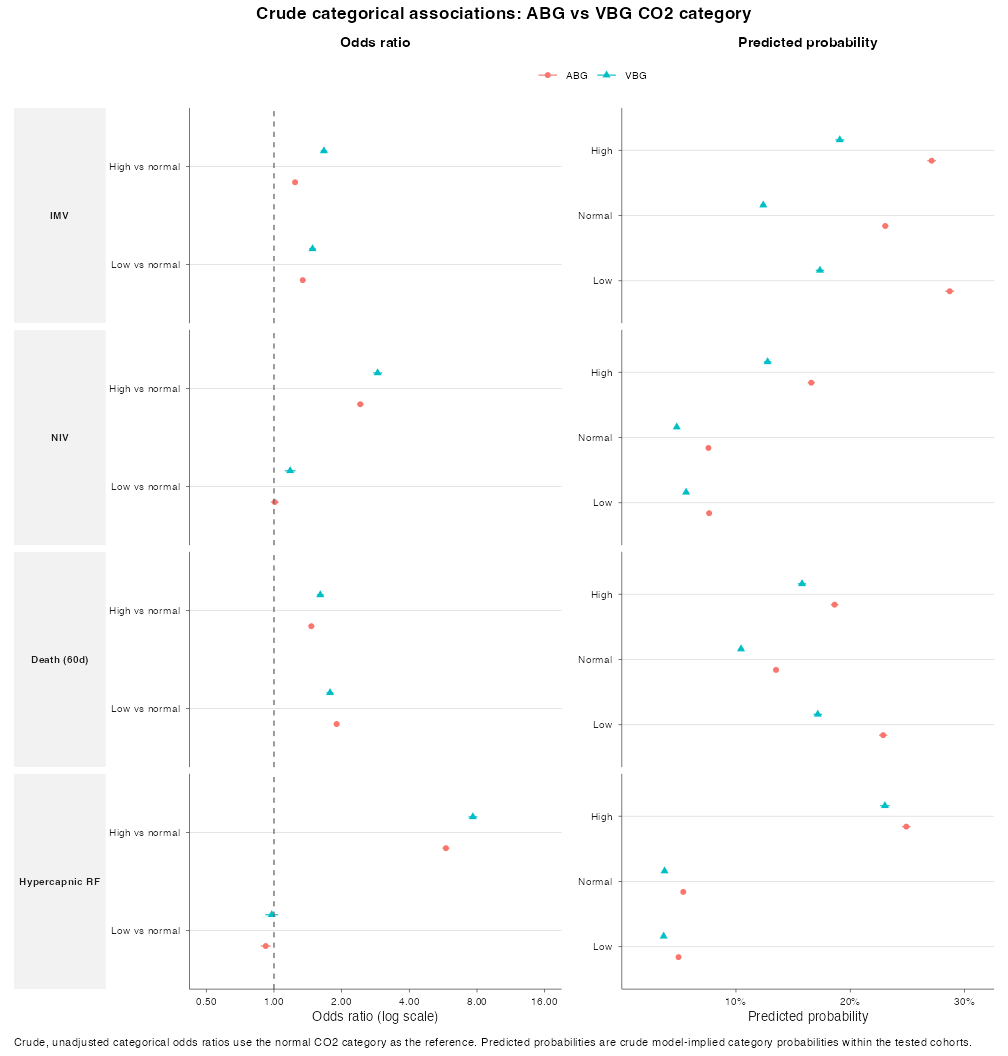
\includegraphics[width=0.94\linewidth,height=0.72\textheight,keepaspectratio]{Results/figs/key-results-cat3-crude-abg-vbg-report-preview.png}
\end{center}

\begin{center}
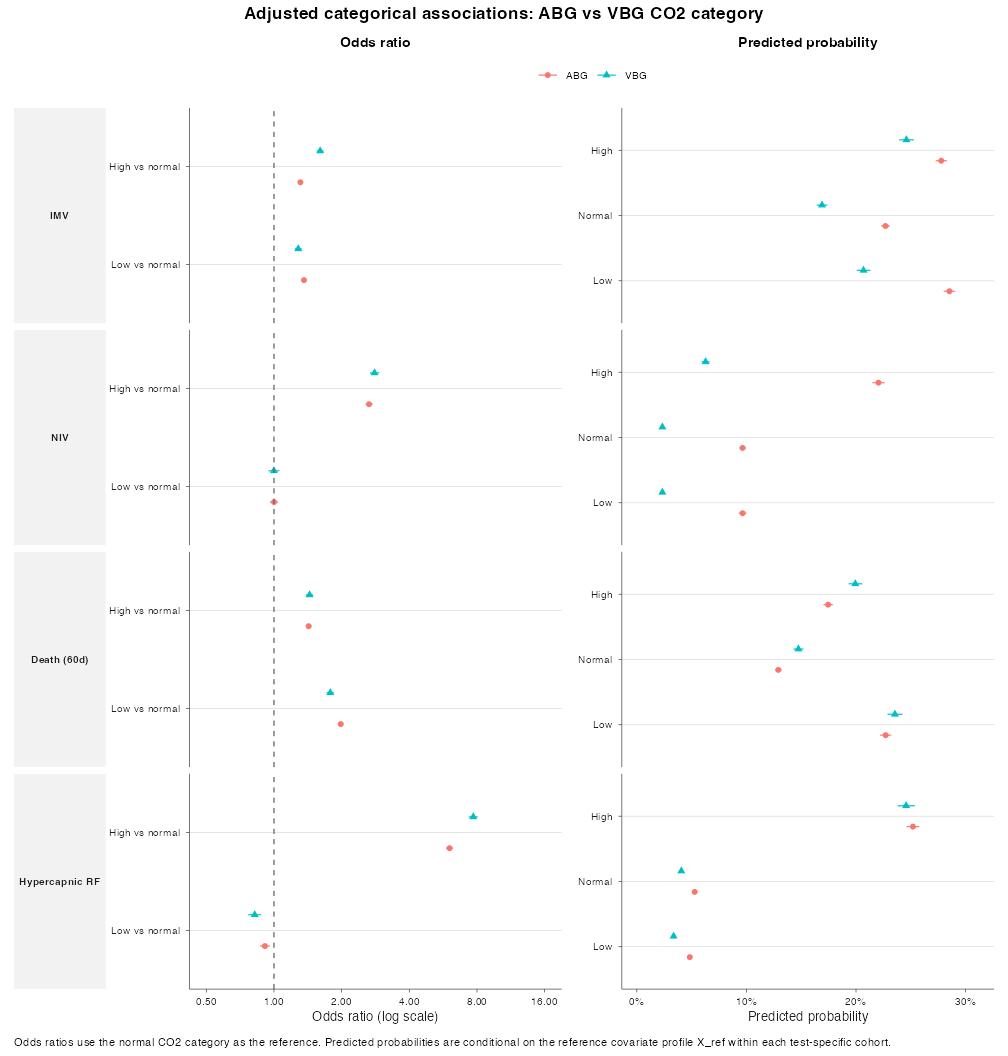
\includegraphics[width=0.94\linewidth,height=0.72\textheight,keepaspectratio]{Results/figs/key-results-cat3-adjusted-abg-vbg-report-preview.png}
\end{center}

\begin{center}
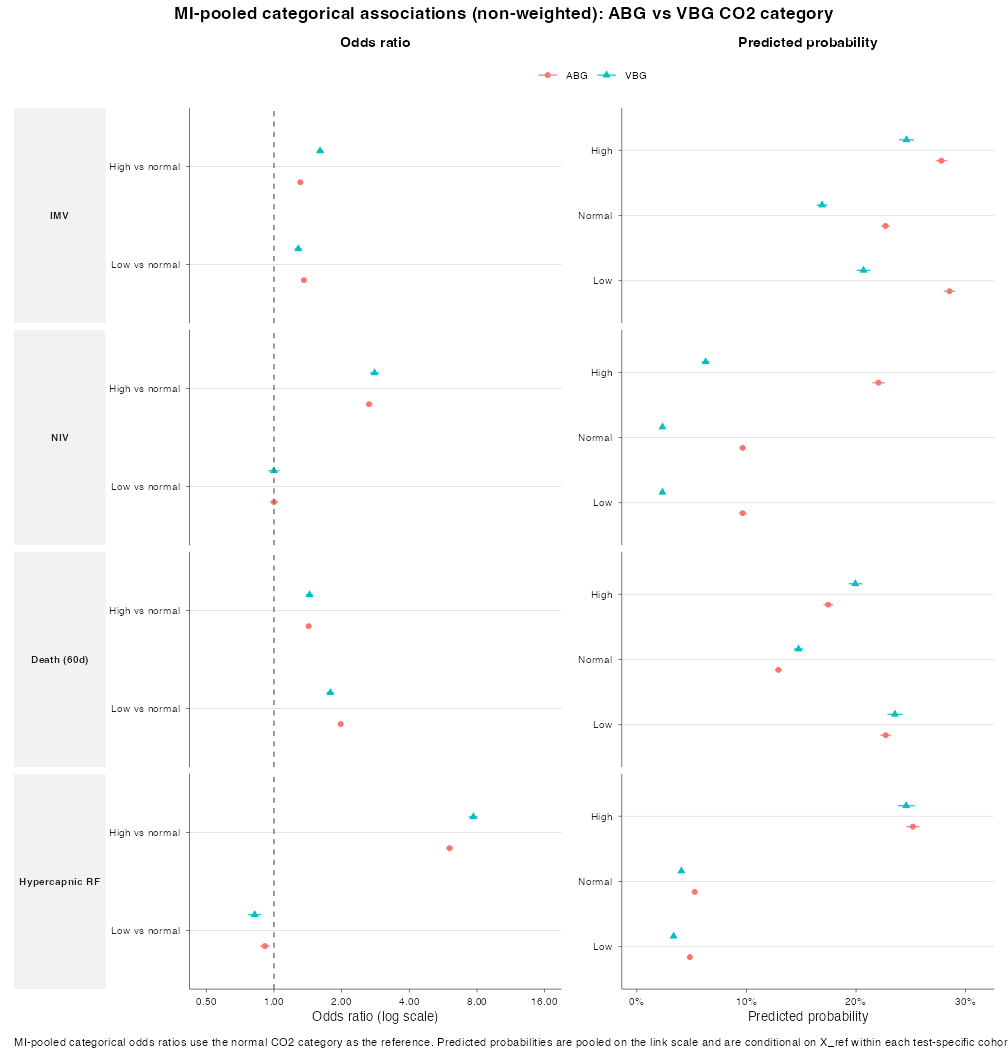
\includegraphics[width=0.94\linewidth,height=0.72\textheight,keepaspectratio]{Results/figs/key-results-cat3-imputed-abg-vbg-report-preview.png}
\end{center}

\begin{center}
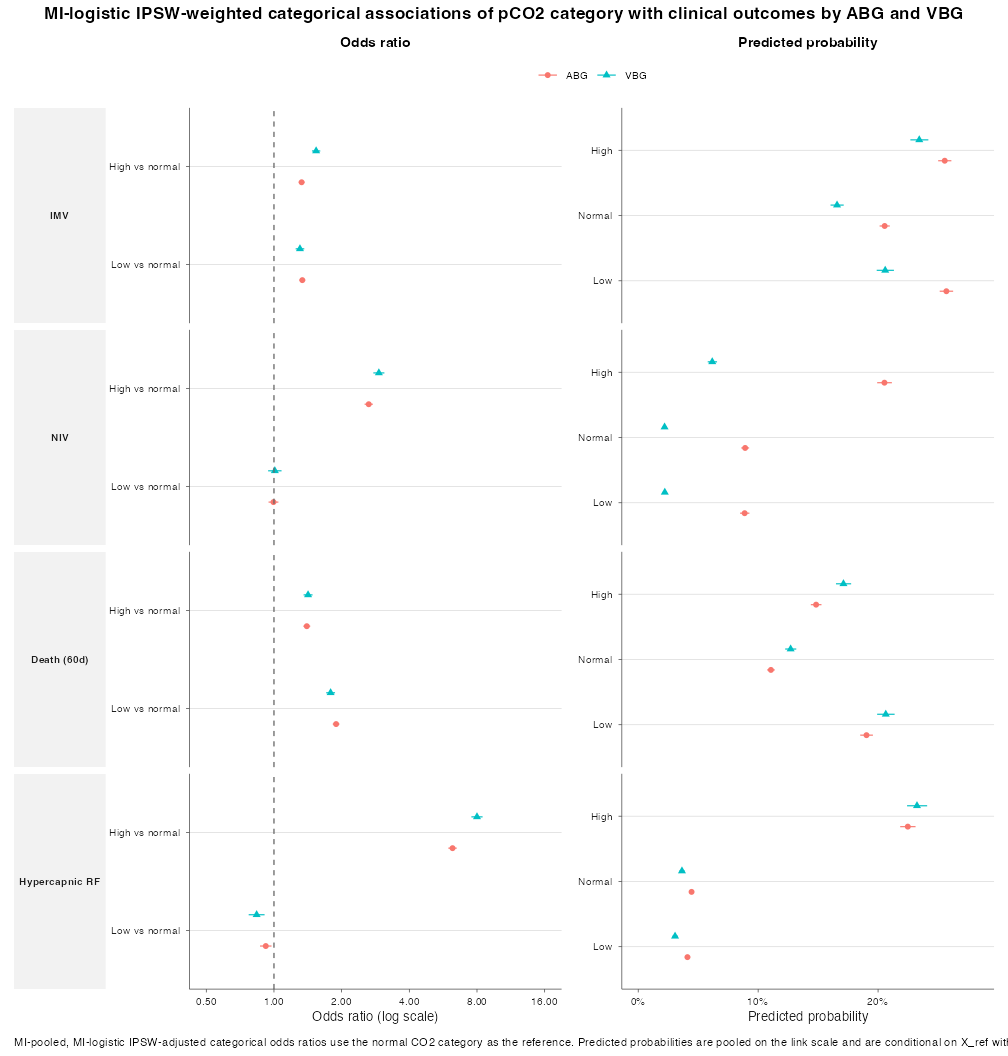
\includegraphics[width=0.94\linewidth,height=0.72\textheight,keepaspectratio]{Results/figs/key-results-cat3-main-mi-ipw-abg-vbg-report-preview.png}
\end{center}

\begin{center}
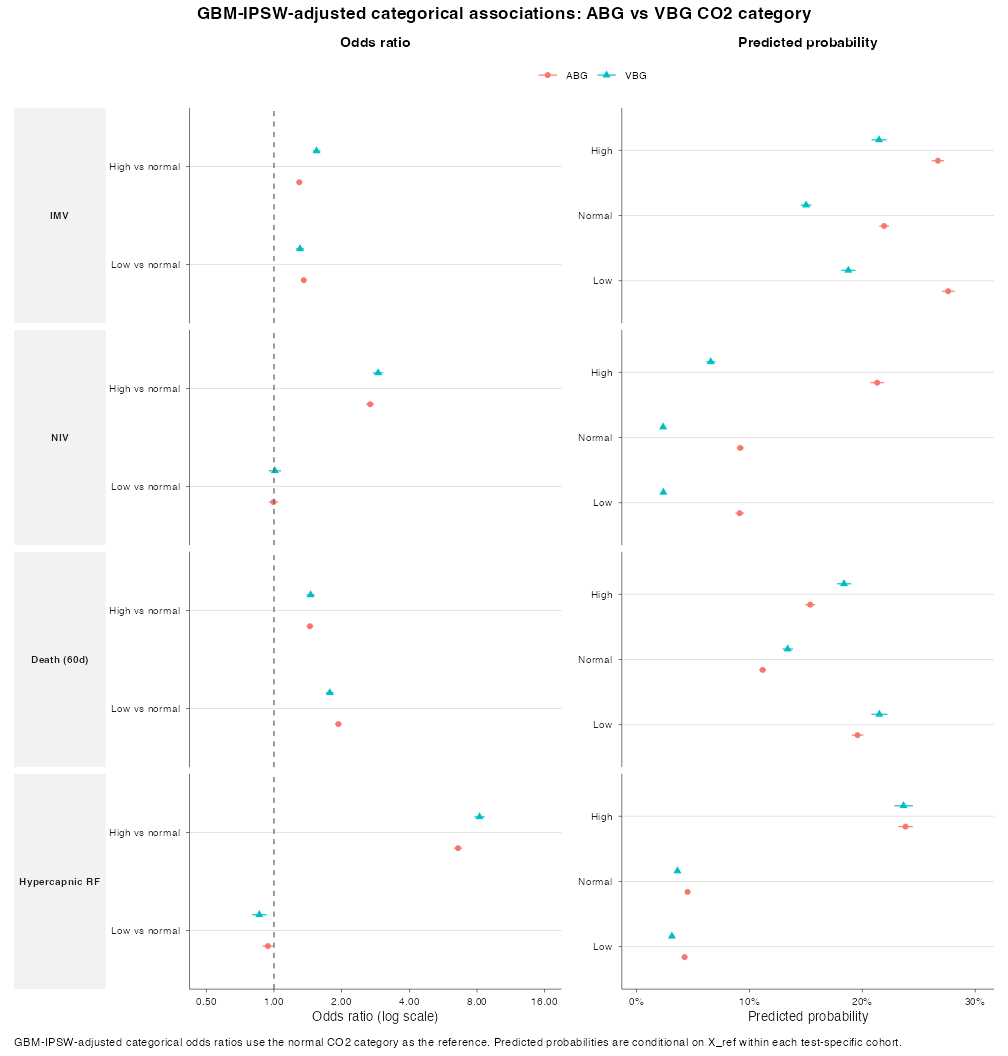
\includegraphics[width=0.94\linewidth,height=0.72\textheight,keepaspectratio]{Results/figs/key-results-cat3-gbm-weighted-abg-vbg-report-preview.png}
\end{center}

\subsection{Observed outcome rates by CO2 bin (MI-logistic
IPSW)}\label{observed-outcome-rates-by-co2-bin-mi-logistic-ipsw}

\begin{center}
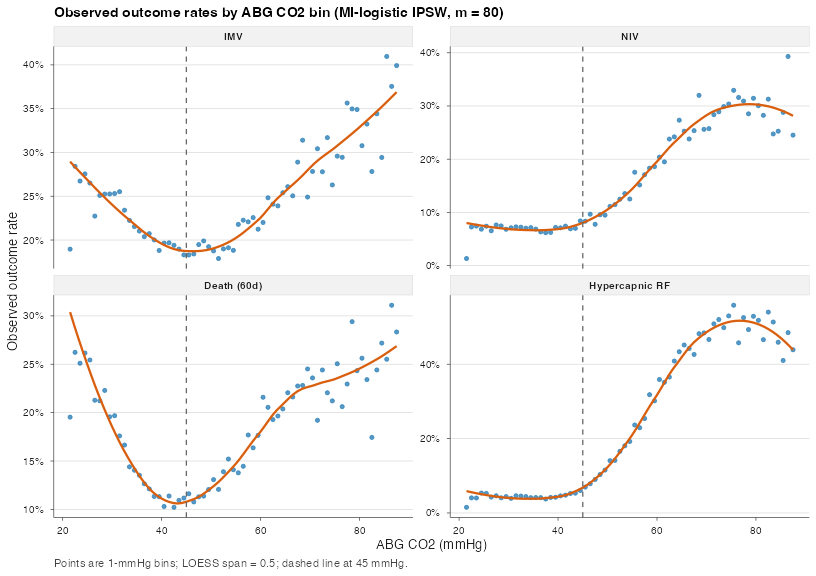
\includegraphics[width=0.94\linewidth,height=0.72\textheight,keepaspectratio]{Results/figs/co2-binned-rates-mi-ipw-abg-report-preview.png}
\end{center}

\begin{center}
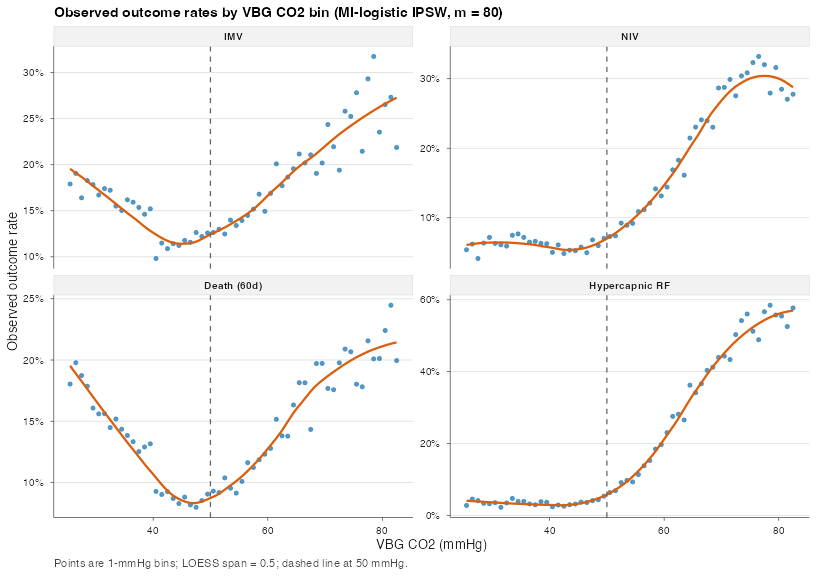
\includegraphics[width=0.94\linewidth,height=0.72\textheight,keepaspectratio]{Results/figs/co2-binned-rates-mi-ipw-vbg-report-preview.png}
\end{center}

\subsection{Manuscript outputs
summary}\label{manuscript-outputs-summary}

\begin{verbatim}

TRUE 
  80 
\end{verbatim}

\subsubsection{Visualization: pooled three-level
ORs}\label{visualization-pooled-three-level-ors}

\begin{center}
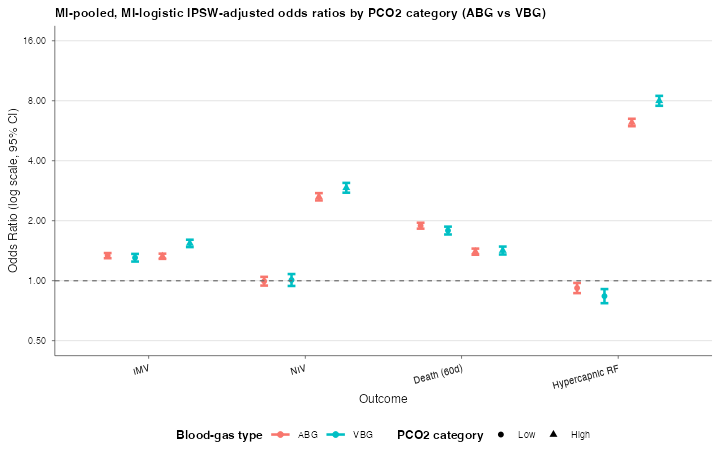
\includegraphics[width=0.94\linewidth,height=0.72\textheight,keepaspectratio]{Results/figs/or-plot-mi-weighted-report-preview.png}
\end{center}

\subsubsection{Visualization: pooled three-level predicted
probabilities}\label{visualization-pooled-three-level-predicted-probabilities}

\begin{center}
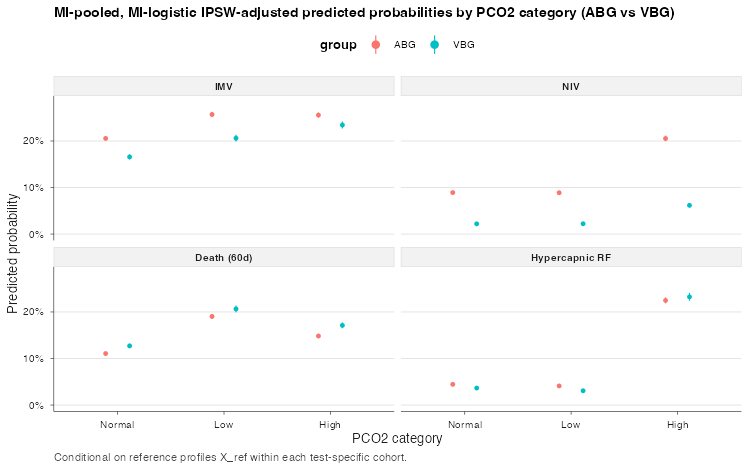
\includegraphics[width=0.94\linewidth,height=0.72\textheight,keepaspectratio]{Results/figs/ipw-three-level-mi-abg-vbg-prob-report-preview.png}
\end{center}

\begin{center}
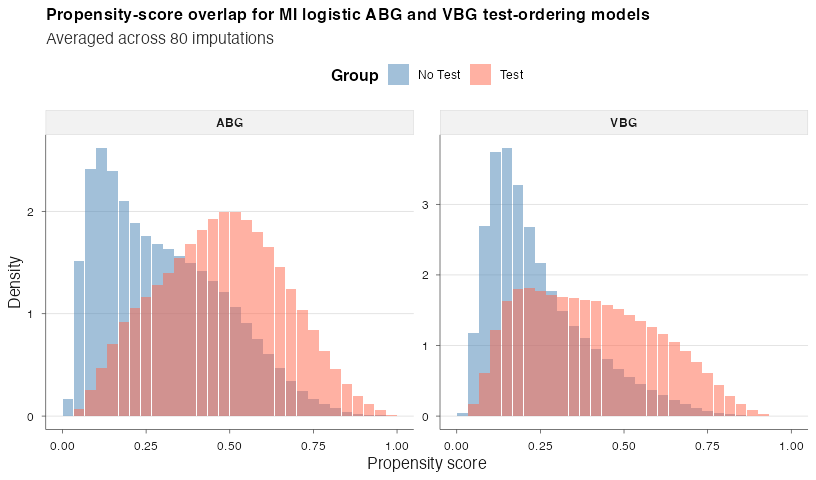
\includegraphics[width=0.94\linewidth,height=0.72\textheight,keepaspectratio]{Results/figs/propensity-histograms-mi-logistic-report-preview.png}
\end{center}

\begin{center}
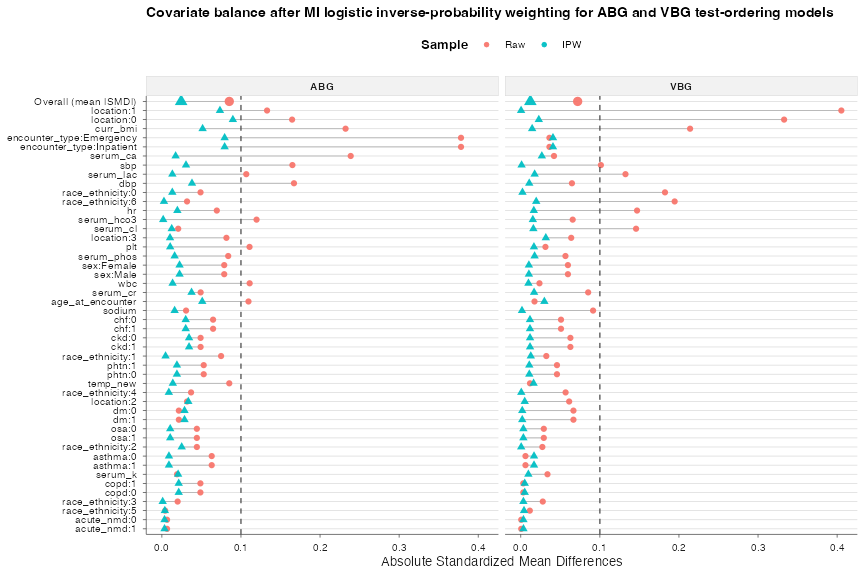
\includegraphics[width=0.94\linewidth,height=0.72\textheight,keepaspectratio]{Results/figs/loveplot-mi-logistic-abg-vbg-report-preview.png}
\end{center}

\begin{center}
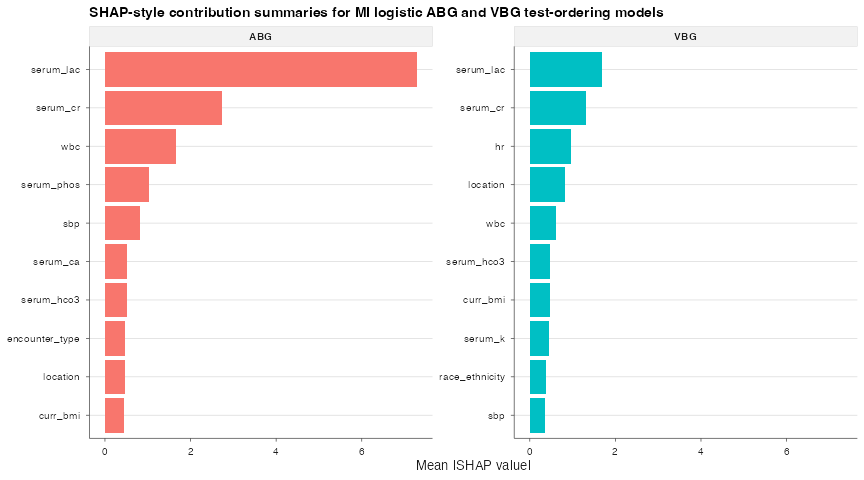
\includegraphics[width=0.94\linewidth,height=0.72\textheight,keepaspectratio]{Results/figs/shap-top10-mi-logistic-abg-vbg-report-preview.png}
\end{center}

\FloatBarrier\nopagebreak

\par

\noindent

\subsubsection{Visualization}\label{visualization}

\begin{center}
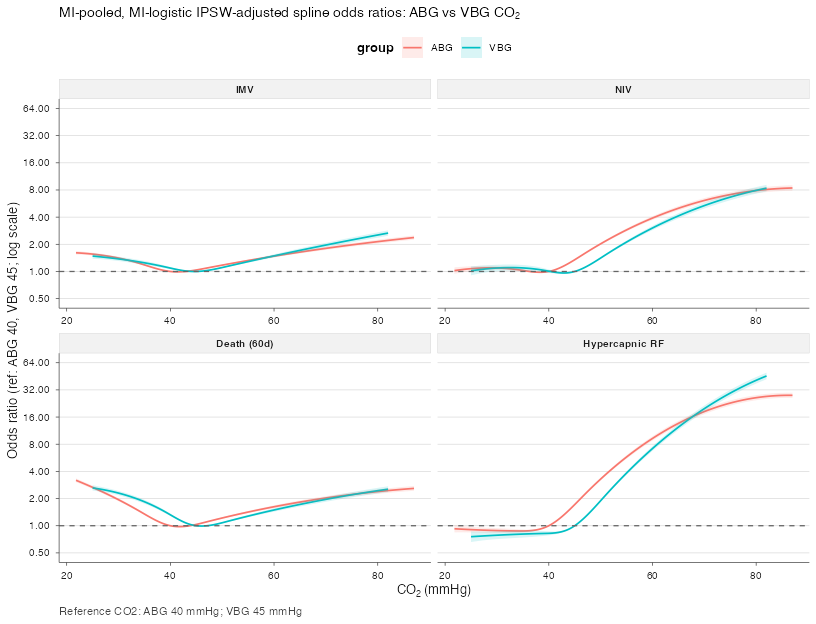
\includegraphics[width=0.94\linewidth,height=0.72\textheight,keepaspectratio]{Results/figs/ipw-rcs-overlay-mi-abg-vbg-report-preview.png}
\end{center}

\begin{center}
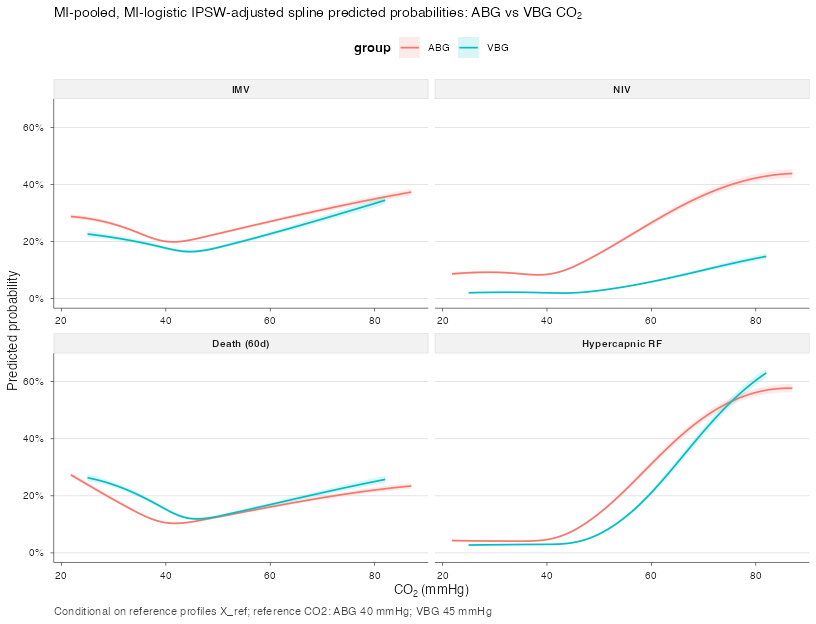
\includegraphics[width=0.94\linewidth,height=0.72\textheight,keepaspectratio]{Results/figs/ipw-rcs-overlay-mi-abg-vbg-prob-report-preview.png}
\end{center}

\subsection{Canonical Key-Results Figures Across Analysis
Tracks}\label{canonical-key-results-figures-across-analysis-tracks}

The following 4×2 figures are the canonical manuscript-facing spline
displays across crude, adjusted, imputed, and weighted analyses.

\begin{center}
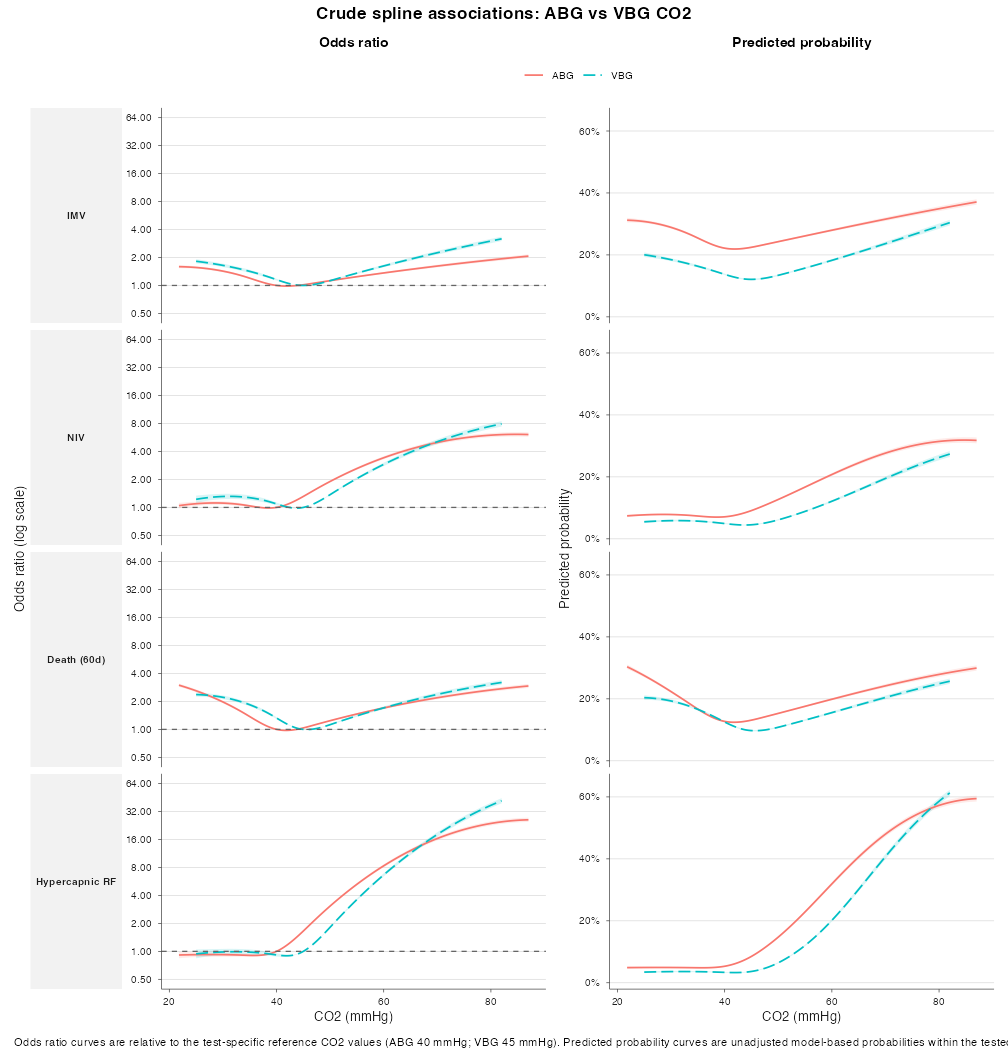
\includegraphics[width=0.94\linewidth,height=0.72\textheight,keepaspectratio]{Results/figs/key-results-spline-crude-abg-vbg-report-preview.png}
\end{center}

\begin{center}
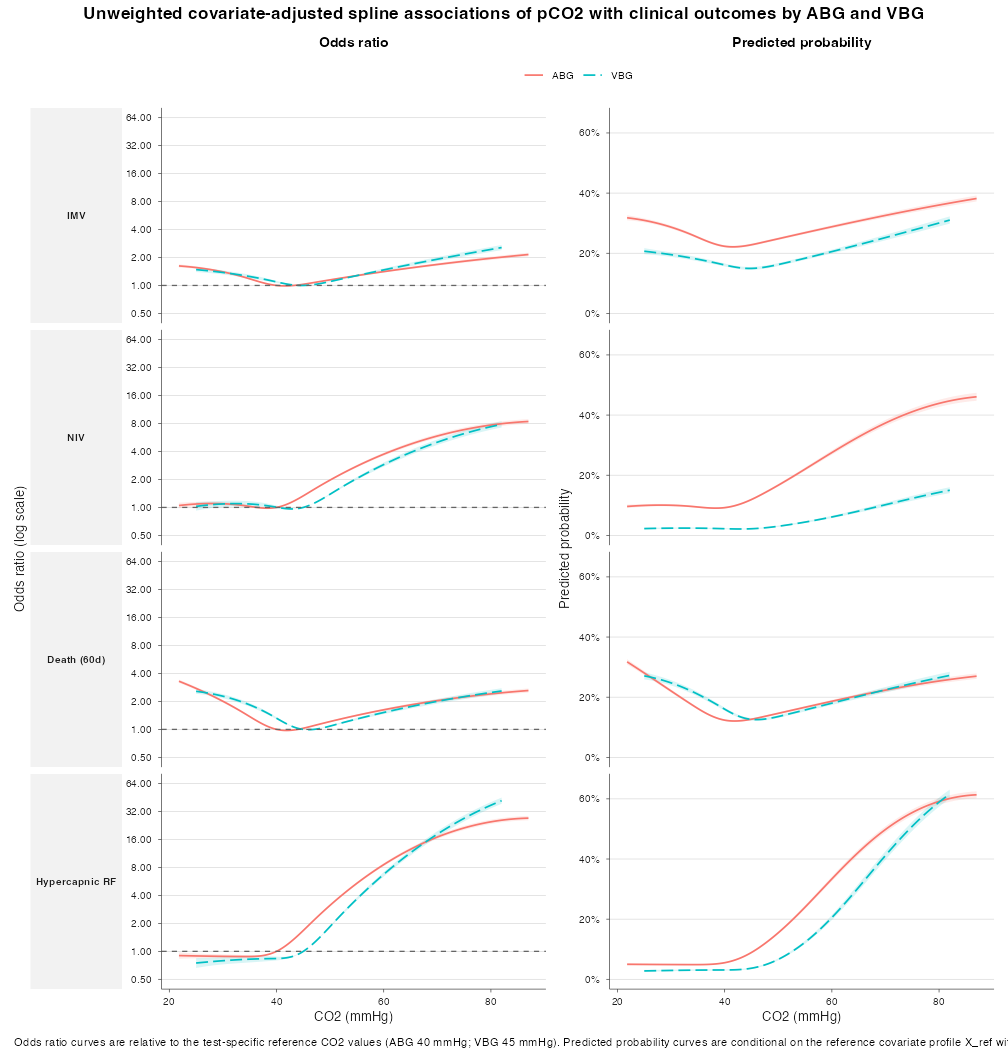
\includegraphics[width=0.94\linewidth,height=0.72\textheight,keepaspectratio]{Results/figs/key-results-spline-adjusted-abg-vbg-report-preview.png}
\end{center}

\begin{center}
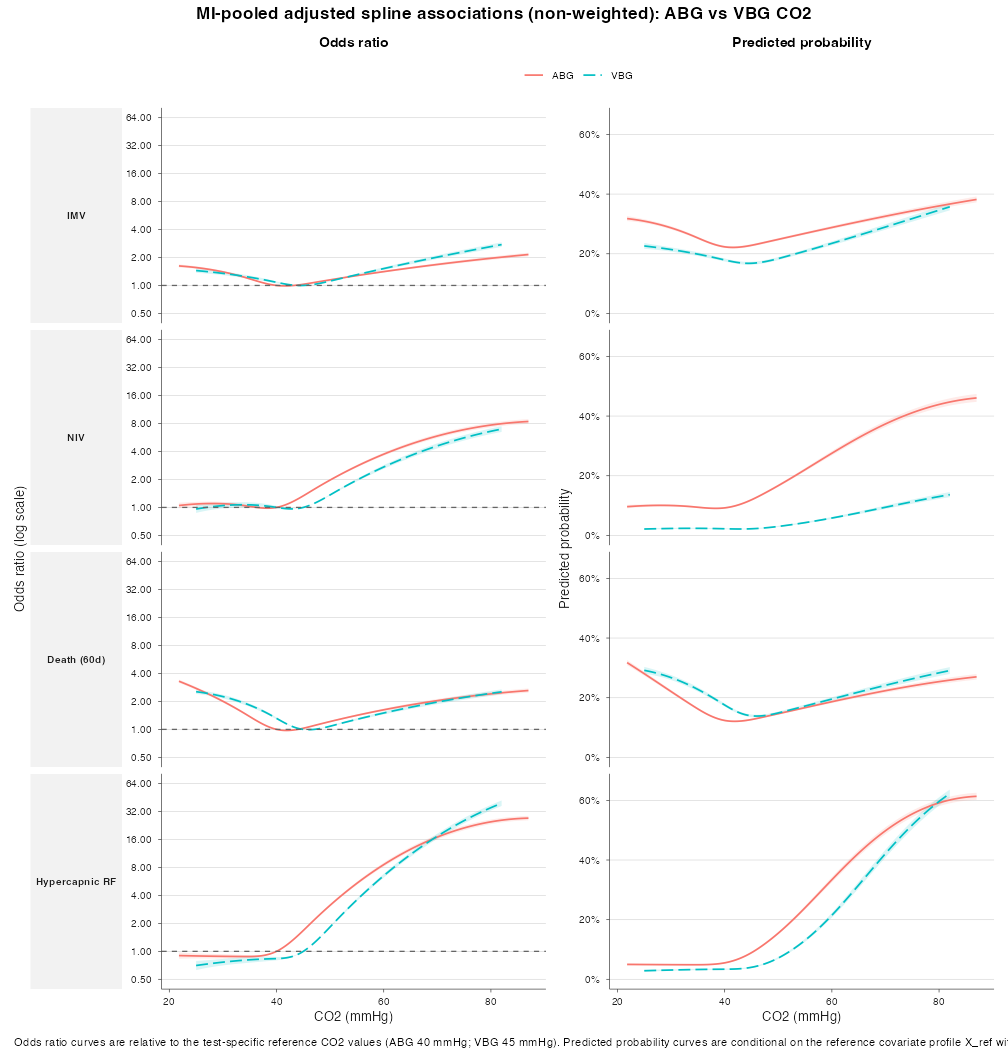
\includegraphics[width=0.94\linewidth,height=0.72\textheight,keepaspectratio]{Results/figs/key-results-spline-imputed-abg-vbg-report-preview.png}
\end{center}

\begin{center}
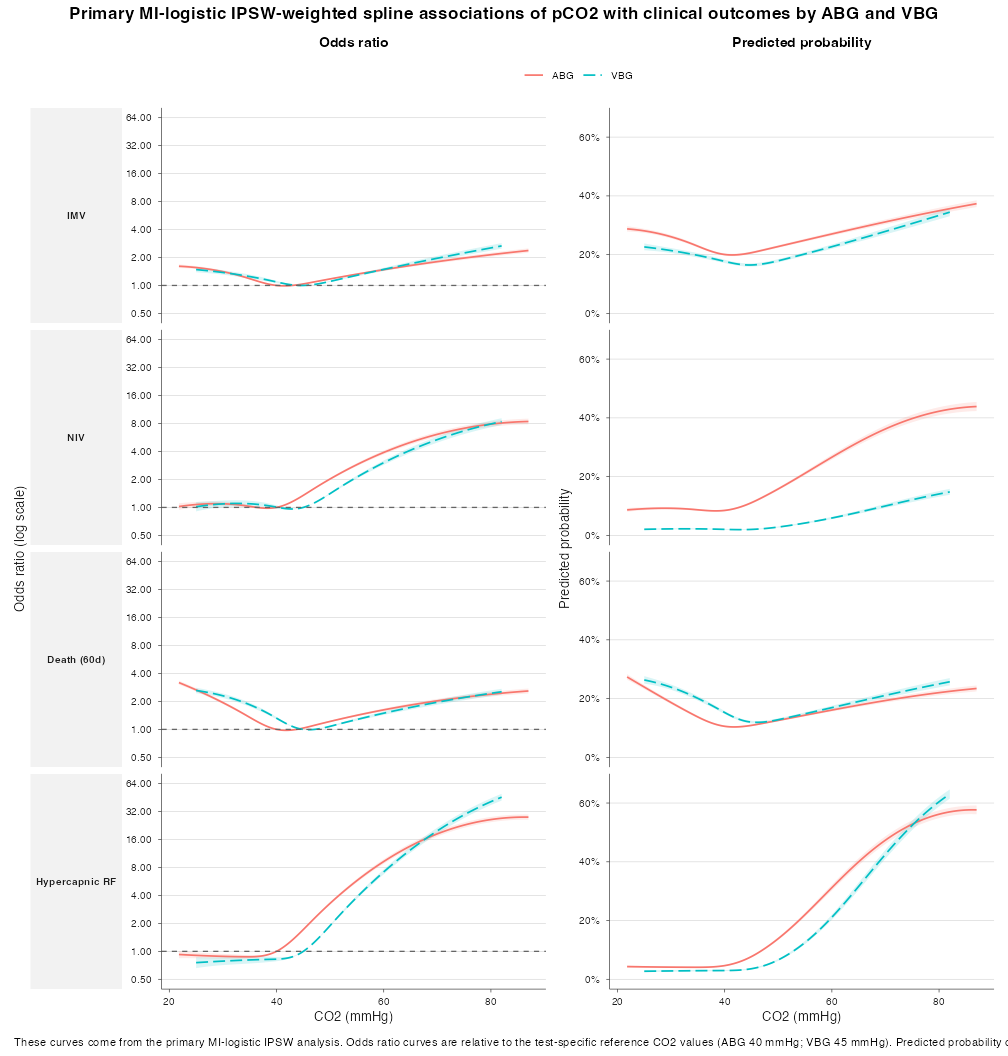
\includegraphics[width=0.94\linewidth,height=0.72\textheight,keepaspectratio]{Results/figs/key-results-spline-main-mi-ipw-abg-vbg-report-preview.png}
\end{center}

\begin{center}
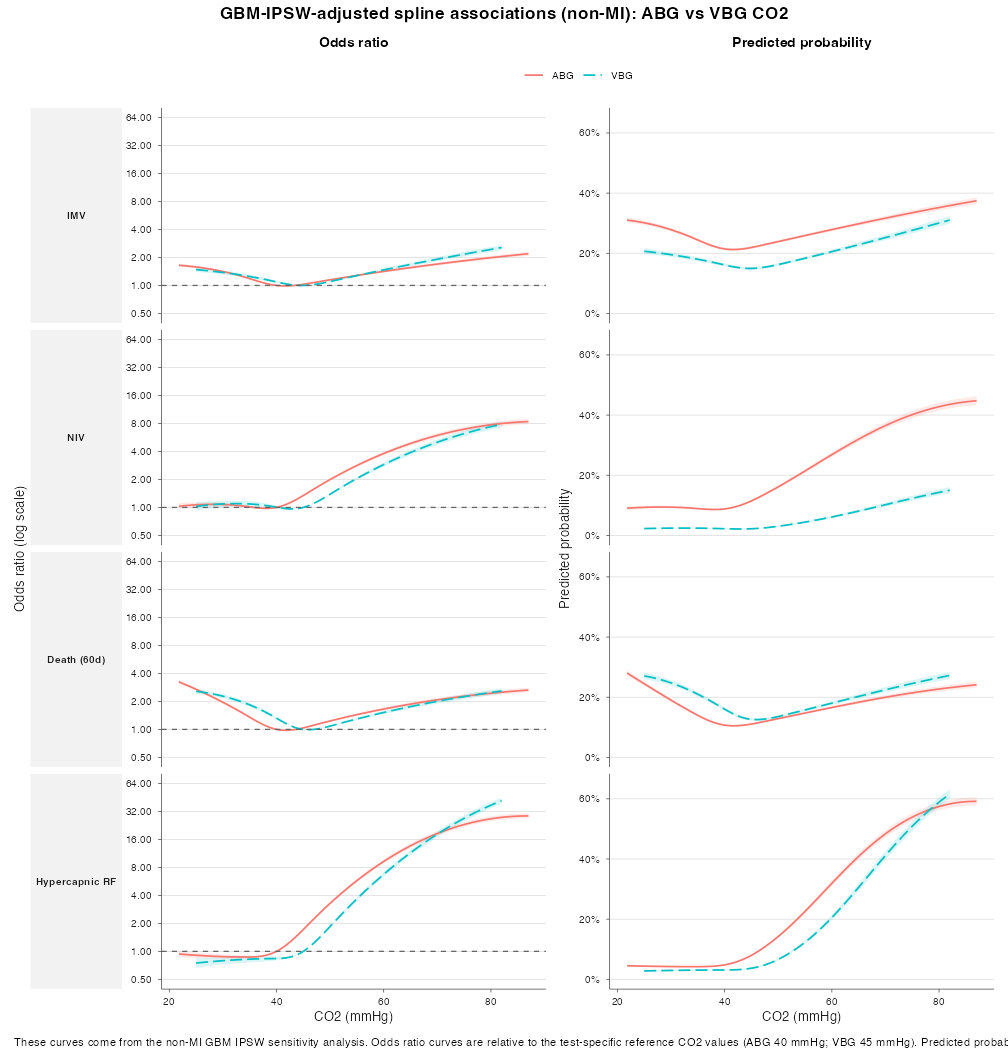
\includegraphics[width=0.94\linewidth,height=0.72\textheight,keepaspectratio]{Results/figs/key-results-spline-gbm-weighted-abg-vbg-report-preview.png}
\end{center}

\FloatBarrier\nopagebreak

\par

\noindent

\begin{longtable}[]{@{}
  >{\raggedright\arraybackslash}p{(\linewidth - 10\tabcolsep) * \real{0.0789}}
  >{\raggedright\arraybackslash}p{(\linewidth - 10\tabcolsep) * \real{0.1447}}
  >{\raggedright\arraybackslash}p{(\linewidth - 10\tabcolsep) * \real{0.0921}}
  >{\raggedright\arraybackslash}p{(\linewidth - 10\tabcolsep) * \real{0.2763}}
  >{\raggedright\arraybackslash}p{(\linewidth - 10\tabcolsep) * \real{0.3618}}
  >{\raggedright\arraybackslash}p{(\linewidth - 10\tabcolsep) * \real{0.0461}}@{}}
\toprule\noalign{}
\begin{minipage}[b]{\linewidth}\raggedright
family
\end{minipage} & \begin{minipage}[b]{\linewidth}\raggedright
track
\end{minipage} & \begin{minipage}[b]{\linewidth}\raggedright
artifact\_type
\end{minipage} & \begin{minipage}[b]{\linewidth}\raggedright
artifact\_name
\end{minipage} & \begin{minipage}[b]{\linewidth}\raggedright
artifact\_path
\end{minipage} & \begin{minipage}[b]{\linewidth}\raggedright
exists
\end{minipage} \\
\midrule\noalign{}
\endhead
\bottomrule\noalign{}
\endlastfoot
Spline & Crude & figure & key-results-spline-crude-abg-vbg.png &
Results/figs/key-results-spline-crude-abg-vbg.png & TRUE \\
Spline & Adjusted & figure & key-results-spline-adjusted-abg-vbg.png &
Results/figs/key-results-spline-adjusted-abg-vbg.png & TRUE \\
Spline & Imputed & figure & key-results-spline-imputed-abg-vbg.png &
Results/figs/key-results-spline-imputed-abg-vbg.png & TRUE \\
Categorical & Crude & figure & key-results-cat3-crude-abg-vbg.png &
Results/figs/key-results-cat3-crude-abg-vbg.png & TRUE \\
Categorical & Adjusted & figure & key-results-cat3-adjusted-abg-vbg.png
& Results/figs/key-results-cat3-adjusted-abg-vbg.png & TRUE \\
Categorical & Imputed & figure & key-results-cat3-imputed-abg-vbg.png &
Results/figs/key-results-cat3-imputed-abg-vbg.png & TRUE \\
Categorical & Weighted and adjusted & figure &
key-results-cat3-main-mi-ipw-abg-vbg.png &
Results/figs/key-results-cat3-main-mi-ipw-abg-vbg.png & TRUE \\
Categorical & GBM-weighted & figure &
key-results-cat3-gbm-weighted-abg-vbg.png &
Results/figs/key-results-cat3-gbm-weighted-abg-vbg.png & TRUE \\
Categorical & Master table & table\_csv &
table\_summary\_key\_results\_cat3.csv &
Results/table\_summary\_key\_results\_cat3.csv & TRUE \\
Categorical & ABG table & table\_csv &
table\_summary\_key\_results\_cat3\_abg.csv &
Results/table\_summary\_key\_results\_cat3\_abg.csv & TRUE \\
Categorical & VBG table & table\_csv &
table\_summary\_key\_results\_cat3\_vbg.csv &
Results/table\_summary\_key\_results\_cat3\_vbg.csv & TRUE \\
Categorical & Long-form extract & table\_csv &
cat3\_key\_results\_long.csv & Results/cat3\_key\_results\_long.csv &
TRUE \\
\end{longtable}

\section{Diagnostics and Exports}\label{diagnostics-and-exports}

\subsubsection{MI convergence and
mixing}\label{mi-convergence-and-mixing}

\begin{verbatim}
png 
  2 
\end{verbatim}

\subsubsection{MI stability across m}\label{mi-stability-across-m}

\subsubsection{MI maxit sensitivity
(sampled)}\label{mi-maxit-sensitivity-sampled}

\subsubsection{Balance diagnostics}\label{balance-diagnostics}

\subsubsection{Outcome diagnostics}\label{outcome-diagnostics}

\subsubsection{Diagnostics summary and
audit}\label{diagnostics-summary-and-audit}

\subsubsection{Performance / runtime log}\label{performance-runtime-log}

\subsubsection{Performance / runtime
log}\label{performance-runtime-log-1}

\subsection{Save, export, and session
info}\label{save-export-and-session-info}

\begin{center}\textbf{Validation build status}\end{center}

\begin{table}[!h]
\centering\begingroup\fontsize{6}{8}\selectfont

\resizebox{\ifdim\width>\linewidth\linewidth\else\width\fi}{!}{
\begin{tabular}{lll}
\toprule
component & status & detail\\
\midrule
overall\_build & FAIL & Final validation status derived from artifact checks, glyph audit, duplicate audit, and diagnostics audit.\\
artifact\_registry & PASS & 0 missing required generated artifact rows.\\
external\_manual\_assets & PASS\_WITH\_WARNINGS & 1 declared external/manual rows.\\
glyph\_audit & PASS & 0 unsafe manuscript glyph rows.\\
duplicate\_audit & PASS & 0 conflicting duplicate/numbering rows.\\
\addlinespace
diagnostics\_audit & FAIL & 1 high / 0 medium / 0 low diagnostics issues.\\
\bottomrule
\end{tabular}}
\endgroup{}
\end{table}\begin{landscape}

\begin{center}\textbf{Artifact provenance summary}\end{center}

\begin{table}[!h]
\centering\begingroup\fontsize{6}{8}\selectfont

\resizebox{\ifdim\width>\linewidth\linewidth\else\width\fi}{!}{
\begin{tabular}{lllllr}
\toprule
section & kind & status & source\_type & pdf\_display & n\_assets\\
\midrule
draft\_only & figure & draft\_only & suppressed/deprecated & FALSE & 1\\
main & figure & generated & notebook\_generated & TRUE & 2\\
main & table & generated & notebook\_generated & TRUE & 2\\
supplement & figure & generated & notebook\_generated & TRUE & 8\\
supplement & table & external/manual & external/manual & FALSE & 1\\
\addlinespace
supplement & table & generated & notebook\_generated & TRUE & 2\\
\bottomrule
\end{tabular}}
\endgroup{}
\end{table}

\end{landscape}\clearpage
\begin{center}
\begin{minipage}{\linewidth}
\centering
\small Figure 1. Cohort assembly and target population for inverse probability-of-sampling weighting\par
\vspace{0.5em}
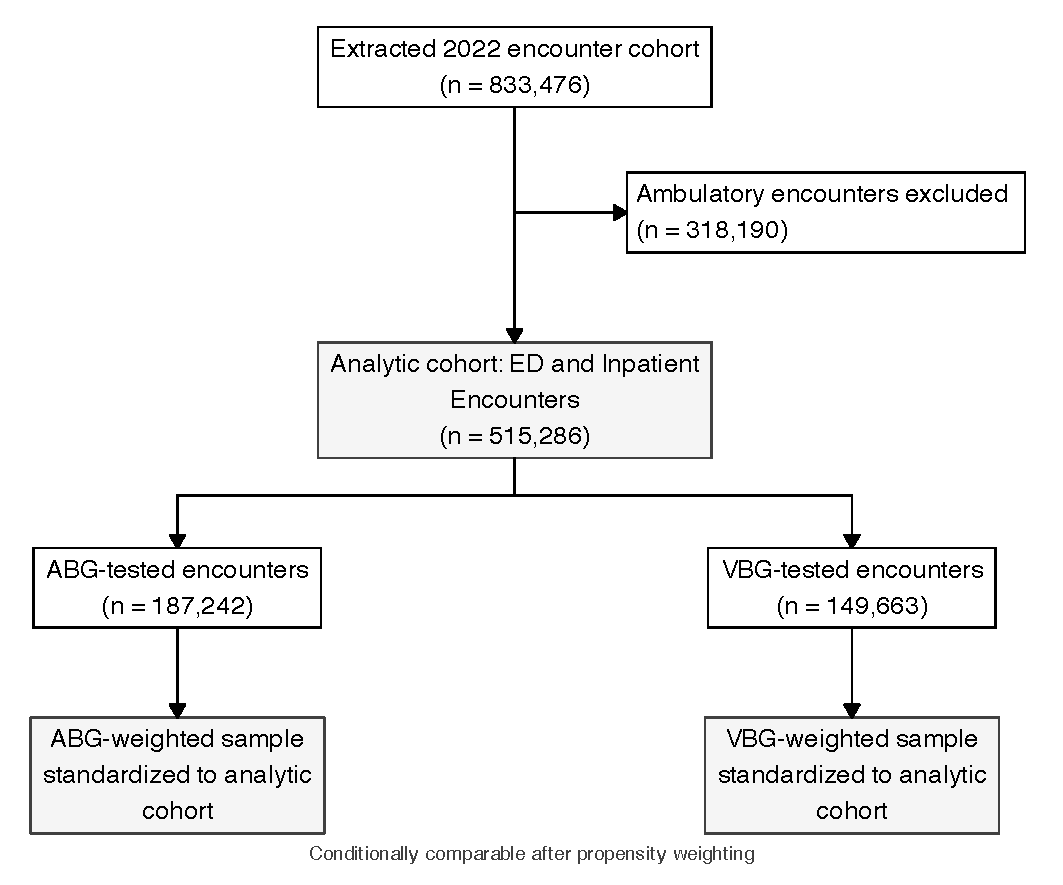
\includegraphics[width=0.88\linewidth,height=0.82\textheight,keepaspectratio]{Results/figs/figure_1_cohort_assembly_target_population_ipsw.pdf}
\end{minipage}
\end{center}

\clearpage
\begin{center}
\begin{minipage}{\linewidth}
\centering
\small Figure 2. Primary MI-logistic IPSW-weighted spline associations of pCO2 with clinical outcomes by ABG and VBG\par
\vspace{0.5em}
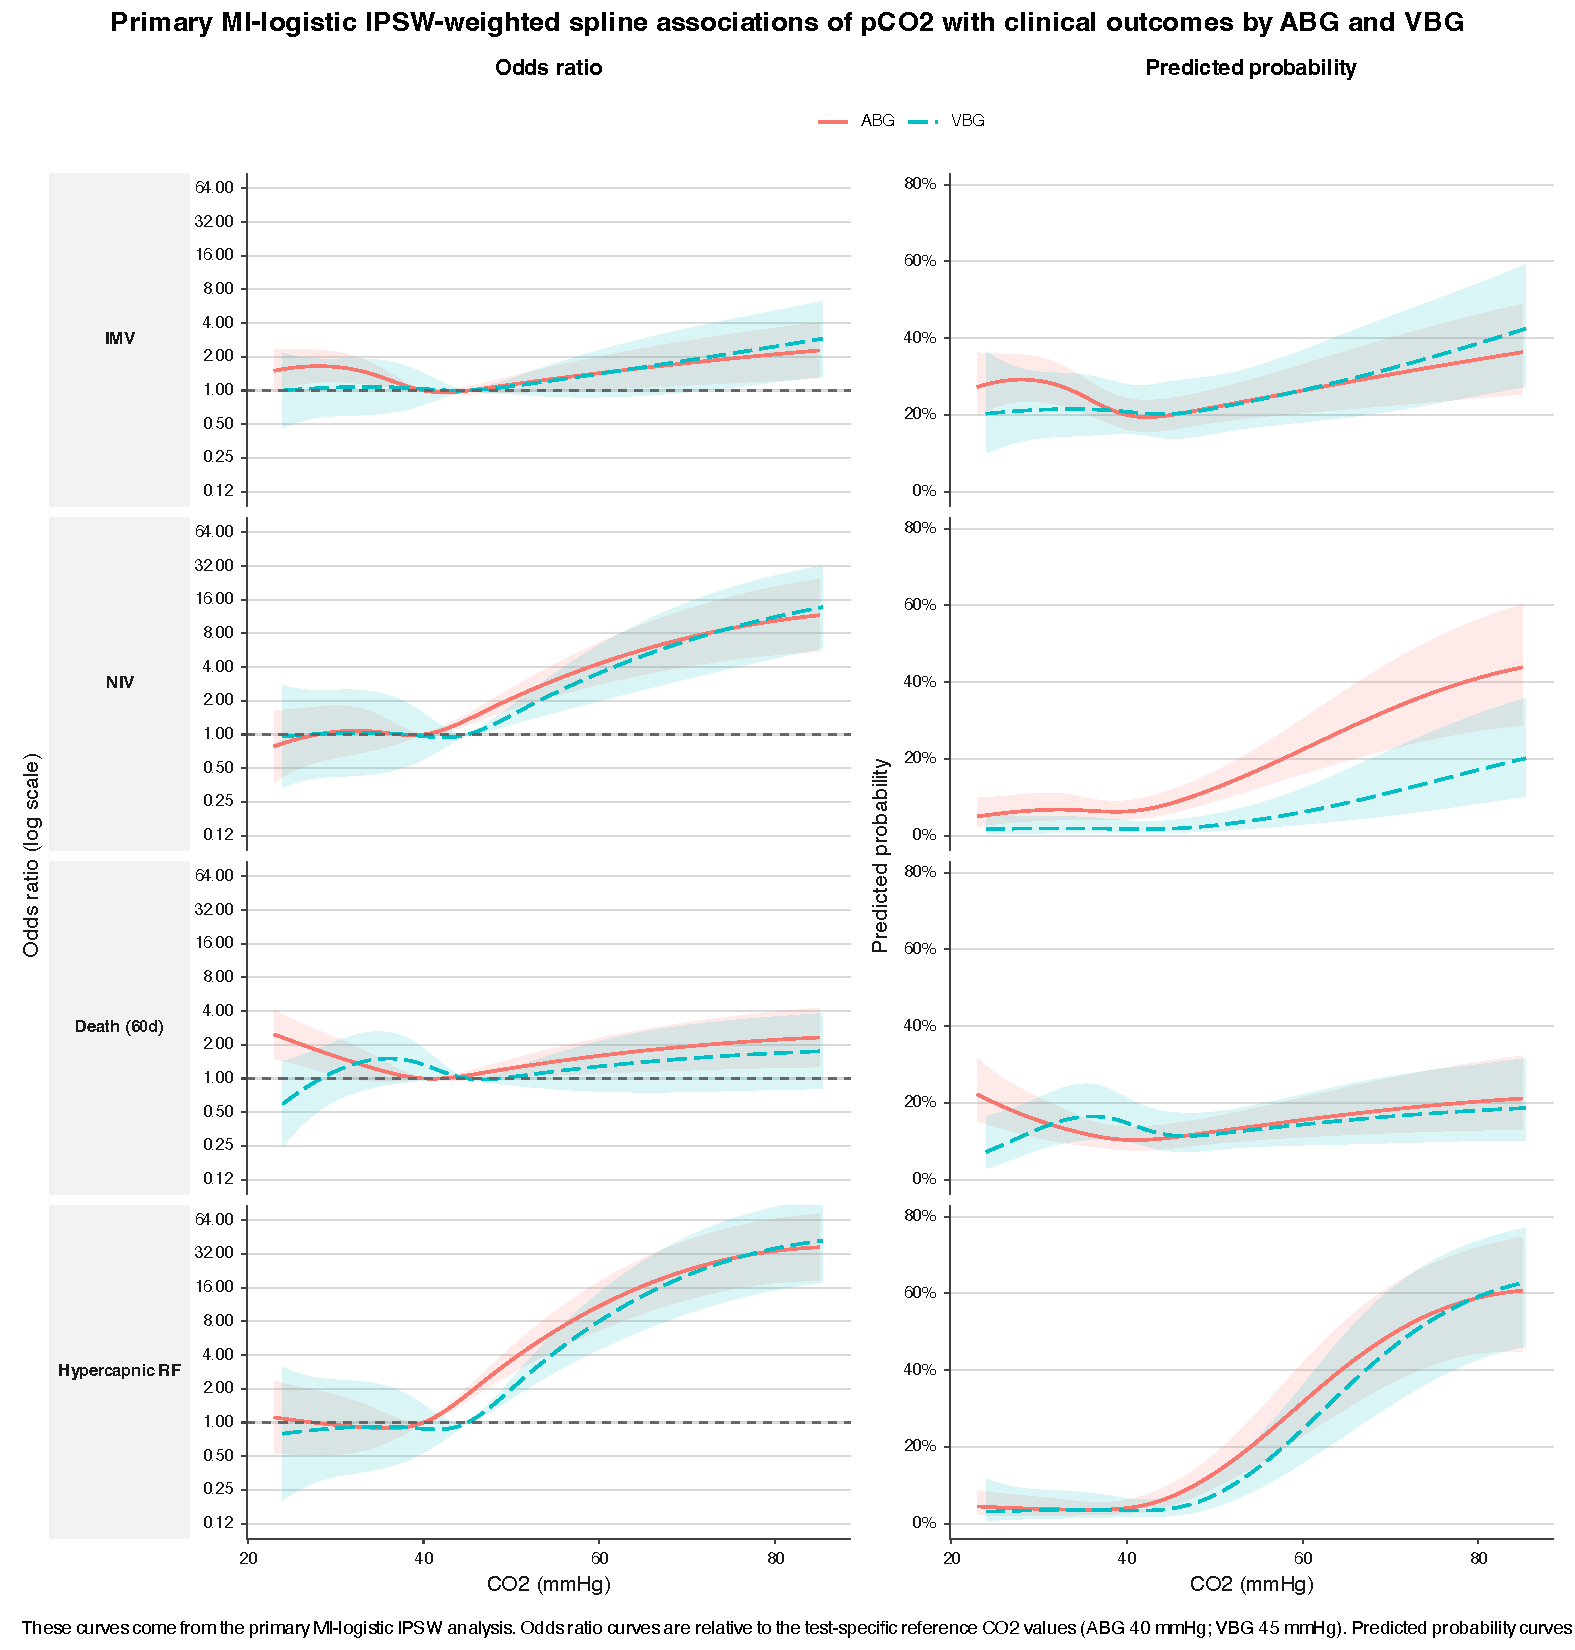
\includegraphics[width=0.88\linewidth,height=0.82\textheight,keepaspectratio]{Results/figs/figure_2_primary_weighted_spline_associations_abg_vbg.pdf}
\end{minipage}
\end{center}

\clearpage

\begin{landscape}

\begin{center}\textbf{Table 1. Baseline characteristics of the analytic cohort overall and by receipt of arterial and venous blood gas testing}\end{center}

\begin{table}[!h]
\centering\begingroup\fontsize{6}{8}\selectfont

\resizebox{\ifdim\width>\linewidth\linewidth\else\width\fi}{!}{
\begin{tabular}{llllllll}
\toprule
panel & variable & var\_type & row\_type & var\_label & label & Everyone & Did not get ABG N = 328,044\\
\midrule
ABG status & age\_at\_encounter & continuous & label & Age & Age & 59.2 ± 17.7; 0.0/515,286.0 missing (0.0\%) & 58.1 ± 18.1; 0.0/328,044.0 missing (0.0\%)\\
ABG status & curr\_bmi & continuous & label & BMI & BMI & 31.1 ± 8.4; 293,545.0/515,286.0 missing (57.0\%) & 32.3 ± 8.7; 184,223.0/328,044.0 missing (56.2\%)\\
ABG status & sex\_label & categorical & label & Sex & Sex & NA & NA\\
ABG status & sex\_label & categorical & level & Sex & Female & 253,906 (49\%) & 169,023 (52\%)\\
ABG status & sex\_label & categorical & level & Sex & Male & 261,380 (51\%) & 159,021 (48\%)\\
\addlinespace
ABG status & race\_ethnicity\_label & categorical & label & Race/Ethnicity & Race/Ethnicity & NA & NA\\
ABG status & race\_ethnicity\_label & categorical & level & Race/Ethnicity & White & 321,174 (62\%) & 200,033 (61\%)\\
ABG status & race\_ethnicity\_label & categorical & level & Race/Ethnicity & Black or African American & 89,697 (17\%) & 62,418 (19\%)\\
ABG status & race\_ethnicity\_label & categorical & level & Race/Ethnicity & Hispanic & 33,769 (6.6\%) & 23,548 (7.2\%)\\
ABG status & race\_ethnicity\_label & categorical & level & Race/Ethnicity & Asian & 8,408 (1.6\%) & 4,880 (1.5\%)\\
\addlinespace
ABG status & race\_ethnicity\_label & categorical & level & Race/Ethnicity & American Indian & 4,055 (0.8\%) & 1,971 (0.6\%)\\
ABG status & race\_ethnicity\_label & categorical & level & Race/Ethnicity & Pacific Islander & 678 (0.1\%) & 460 (0.1\%)\\
ABG status & race\_ethnicity\_label & categorical & level & Race/Ethnicity & Unknown & 57,505 (11\%) & 34,734 (11\%)\\
ABG status & location\_label & categorical & label & Location & Location & NA & NA\\
ABG status & location\_label & categorical & level & Location & South & 242,266 (47\%) & 138,843 (42\%)\\
\addlinespace
ABG status & location\_label & categorical & level & Location & Northeast & 129,446 (25\%) & 93,209 (28\%)\\
ABG status & location\_label & categorical & level & Location & Midwest & 38,471 (7.5\%) & 22,924 (7.0\%)\\
ABG status & location\_label & categorical & level & Location & West & 105,103 (20\%) & 73,068 (22\%)\\
ABG status & osa\_label & dichotomous & label & OSA & OSA & 90,327 (18\%) & 60,653 (18\%)\\
ABG status & asthma\_label & dichotomous & label & Asthma & Asthma & 69,773 (14\%) & 48,456 (15\%)\\
\addlinespace
ABG status & copd\_label & dichotomous & label & COPD & COPD & 100,255 (19\%) & 60,214 (18\%)\\
ABG status & chf\_label & dichotomous & label & CHF & CHF & 101,458 (20\%) & 59,770 (18\%)\\
ABG status & nmd\_label & dichotomous & label & NMD & NMD & 20,239 (3.9\%) & 11,891 (3.6\%)\\
ABG status & phtn\_label & dichotomous & label & PHTN & PHTN & 41,714 (8.1\%) & 23,854 (7.3\%)\\
ABG status & ckd\_label & dichotomous & label & CKD & CKD & 91,146 (18\%) & 54,528 (17\%)\\
\addlinespace
ABG status & diabetes\_label & dichotomous & label & Diabetes & Diabetes & 148,954 (29\%) & 93,007 (28\%)\\
ABG status & encounter\_type\_label & categorical & label & Encounter Type & Encounter Type & NA & NA\\
ABG status & encounter\_type\_label & categorical & level & Encounter Type & Emergency & 171,727 (33\%) & 142,713 (44\%)\\
ABG status & encounter\_type\_label & categorical & level & Encounter Type & Inpatient & 343,559 (67\%) & 185,331 (56\%)\\
\bottomrule
\end{tabular}}
\endgroup{}
\end{table}

\begin{table}[!h]
\centering\begingroup\fontsize{6}{8}\selectfont

\resizebox{\ifdim\width>\linewidth\linewidth\else\width\fi}{!}{
\begin{tabular}{lll}
\toprule
Did get ABG N = 187,242 & Did not get VBG N = 365,623 & Did get VBG N = 149,663\\
\midrule
61.2 ± 16.9; 0.0/187,242.0 missing (0.0\%) & 59.4 ± 17.8; 0.0/365,623.0 missing (0.0\%) & 58.9 ± 17.5; 0.0/149,663.0 missing (0.0\%)\\
29.0 ± 7.2; 109,322.0/187,242.0 missing (58.4\%) & 31.8 ± 8.5; 192,892.0/365,623.0 missing (52.8\%) & 28.8 ± 7.4; 100,653.0/149,663.0 missing (67.3\%)\\
NA & NA & NA\\
84,883 (45\%) & 184,619 (50\%) & 69,287 (46\%)\\
102,359 (55\%) & 181,004 (50\%) & 80,376 (54\%)\\
\addlinespace
NA & NA & NA\\
121,141 (65\%) & 241,114 (66\%) & 80,060 (53\%)\\
27,279 (15\%) & 61,814 (17\%) & 27,883 (19\%)\\
10,221 (5.5\%) & 22,951 (6.3\%) & 10,818 (7.2\%)\\
3,528 (1.9\%) & 5,439 (1.5\%) & 2,969 (2.0\%)\\
\addlinespace
2,084 (1.1\%) & 2,128 (0.6\%) & 1,927 (1.3\%)\\
218 (0.1\%) & 543 (0.1\%) & 135 (<0.1\%)\\
22,771 (12\%) & 31,634 (8.7\%) & 25,871 (17\%)\\
NA & NA & NA\\
103,423 (55\%) & 196,774 (54\%) & 45,492 (30\%)\\
\addlinespace
36,237 (19\%) & 65,537 (18\%) & 63,909 (43\%)\\
15,547 (8.3\%) & 24,891 (6.8\%) & 13,580 (9.1\%)\\
32,035 (17\%) & 78,421 (21\%) & 26,682 (18\%)\\
29,674 (16\%) & 65,748 (18\%) & 24,579 (16\%)\\
21,317 (11\%) & 49,810 (14\%) & 19,963 (13\%)\\
\addlinespace
40,041 (21\%) & 70,950 (19\%) & 29,305 (20\%)\\
41,688 (22\%) & 68,964 (19\%) & 32,494 (22\%)\\
8,348 (4.5\%) & 14,796 (4.0\%) & 5,443 (3.6\%)\\
17,860 (9.5\%) & 27,731 (7.6\%) & 13,983 (9.3\%)\\
36,618 (20\%) & 61,091 (17\%) & 30,055 (20\%)\\
\addlinespace
55,947 (30\%) & 101,173 (28\%) & 47,781 (32\%)\\
NA & NA & NA\\
29,014 (15\%) & 124,405 (34\%) & 47,322 (32\%)\\
158,228 (85\%) & 241,218 (66\%) & 102,341 (68\%)\\
\bottomrule
\end{tabular}}
\endgroup{}
\end{table}

\end{landscape}

\clearpage

\begin{landscape}

\begin{center}\textbf{Table 2. MI-pooled, MI-logistic IPSW-weighted 3-level categorical results for ABG and VBG}\end{center}

\begin{table}[!h]
\centering\begingroup\fontsize{6}{8}\selectfont

\resizebox{\ifdim\width>\linewidth\linewidth\else\width\fi}{!}{
\begin{tabular}{llrrllll}
\toprule
group & outcome & n\_model & events & Low vs normal OR (95\% CI) & High vs normal OR (95\% CI) & Normal probability (95\% CI) & Low probability (95\% CI)\\
\midrule
ABG & IMV & 187242 & 48173 & 1.34 (1.30, 1.38) & 1.33 (1.29, 1.37) & 0.21 (0.20, 0.21) & 0.26 (0.25, 0.26)\\
ABG & NIV & 187242 & 19040 & 0.99 (0.95, 1.05) & 2.64 (2.53, 2.75) & 0.09 (0.09, 0.09) & 0.09 (0.08, 0.09)\\
ABG & Death (60d) & 187242 & 32718 & 1.89 (1.83, 1.96) & 1.40 (1.35, 1.45) & 0.11 (0.11, 0.11) & 0.19 (0.19, 0.20)\\
ABG & Hypercapnic RF & 187242 & 20276 & 0.92 (0.87, 0.98) & 6.23 (5.97, 6.50) & 0.04 (0.04, 0.05) & 0.04 (0.04, 0.04)\\
VBG & IMV & 149663 & 23217 & 1.31 (1.25, 1.36) & 1.54 (1.48, 1.61) & 0.17 (0.16, 0.17) & 0.21 (0.20, 0.21)\\
\addlinespace
VBG & NIV & 149663 & 10699 & 1.01 (0.94, 1.08) & 2.93 (2.77, 3.10) & 0.02 (0.02, 0.02) & 0.02 (0.02, 0.02)\\
VBG & Death (60d) & 149663 & 20483 & 1.79 (1.71, 1.87) & 1.42 (1.35, 1.48) & 0.13 (0.12, 0.13) & 0.21 (0.20, 0.21)\\
VBG & Hypercapnic RF & 149663 & 13228 & 0.84 (0.77, 0.91) & 8.00 (7.55, 8.47) & 0.04 (0.03, 0.04) & 0.03 (0.03, 0.03)\\
\bottomrule
\end{tabular}}
\endgroup{}
\end{table}

\begin{table}[!h]
\centering\begingroup\fontsize{6}{8}\selectfont

\resizebox{\ifdim\width>\linewidth\linewidth\else\width\fi}{!}{
\begin{tabular}{l}
\toprule
High probability (95\% CI)\\
\midrule
0.26 (0.25, 0.26)\\
0.21 (0.20, 0.21)\\
0.15 (0.14, 0.15)\\
0.22 (0.22, 0.23)\\
0.23 (0.23, 0.24)\\
\addlinespace
0.06 (0.06, 0.07)\\
0.17 (0.16, 0.18)\\
0.23 (0.22, 0.24)\\
\bottomrule
\end{tabular}}
\endgroup{}
\end{table}

\end{landscape}

\clearpage
\begin{center}
\begin{minipage}{\linewidth}
\centering
\small Figure S1. Covariate balance after MI logistic inverse-probability weighting for ABG and VBG test-ordering models\par
\vspace{0.5em}
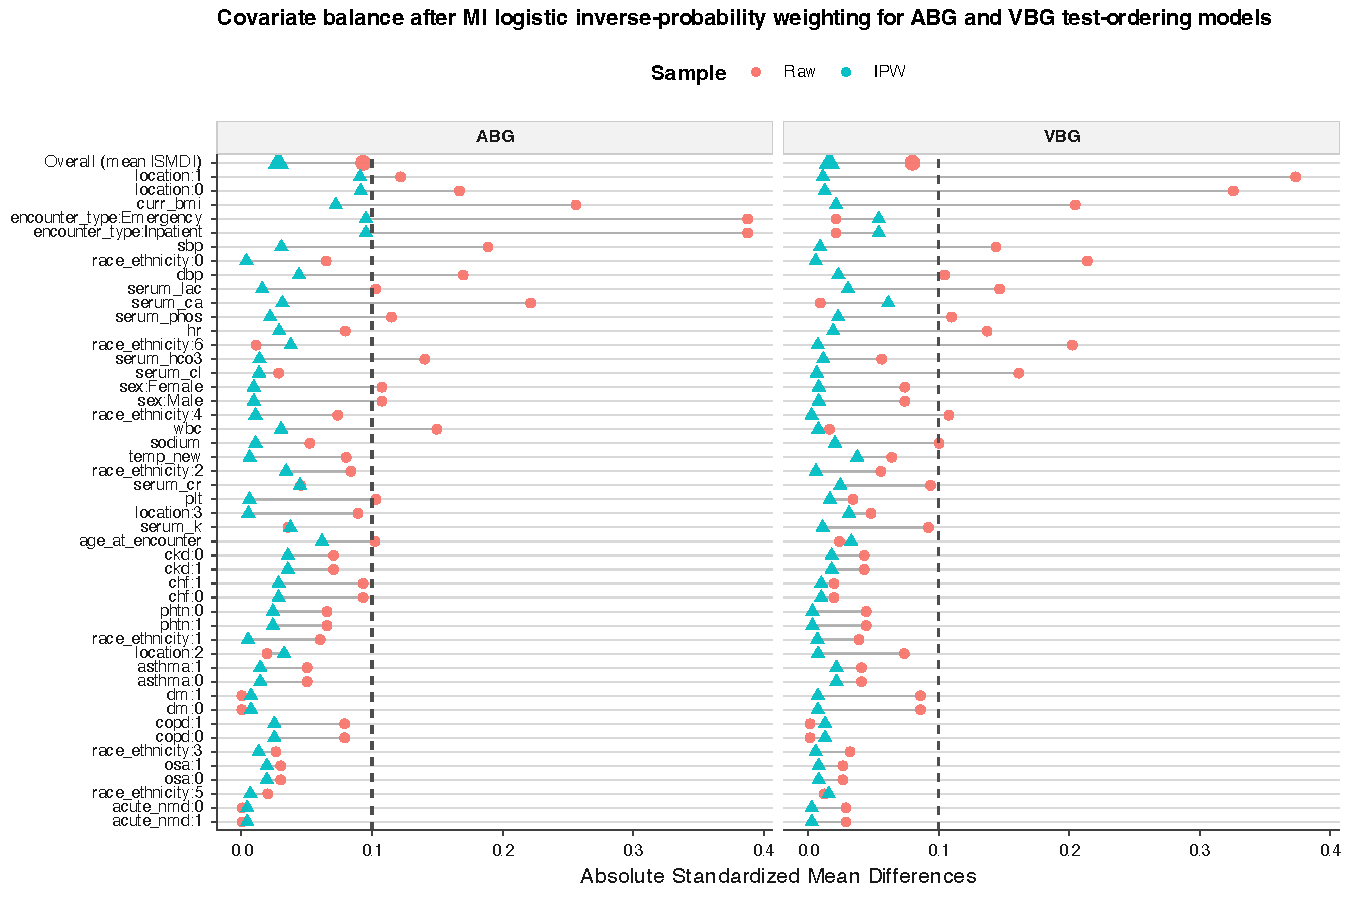
\includegraphics[width=0.88\linewidth,height=0.82\textheight,keepaspectratio]{Results/figs/figure_s1_covariate_balance_mi_logistic_ipsw.pdf}
\end{minipage}
\end{center}

\clearpage
\begin{center}
\begin{minipage}{\linewidth}
\centering
\small Figure S2. Propensity-score overlap for MI logistic ABG and VBG test-ordering models\par
\vspace{0.5em}
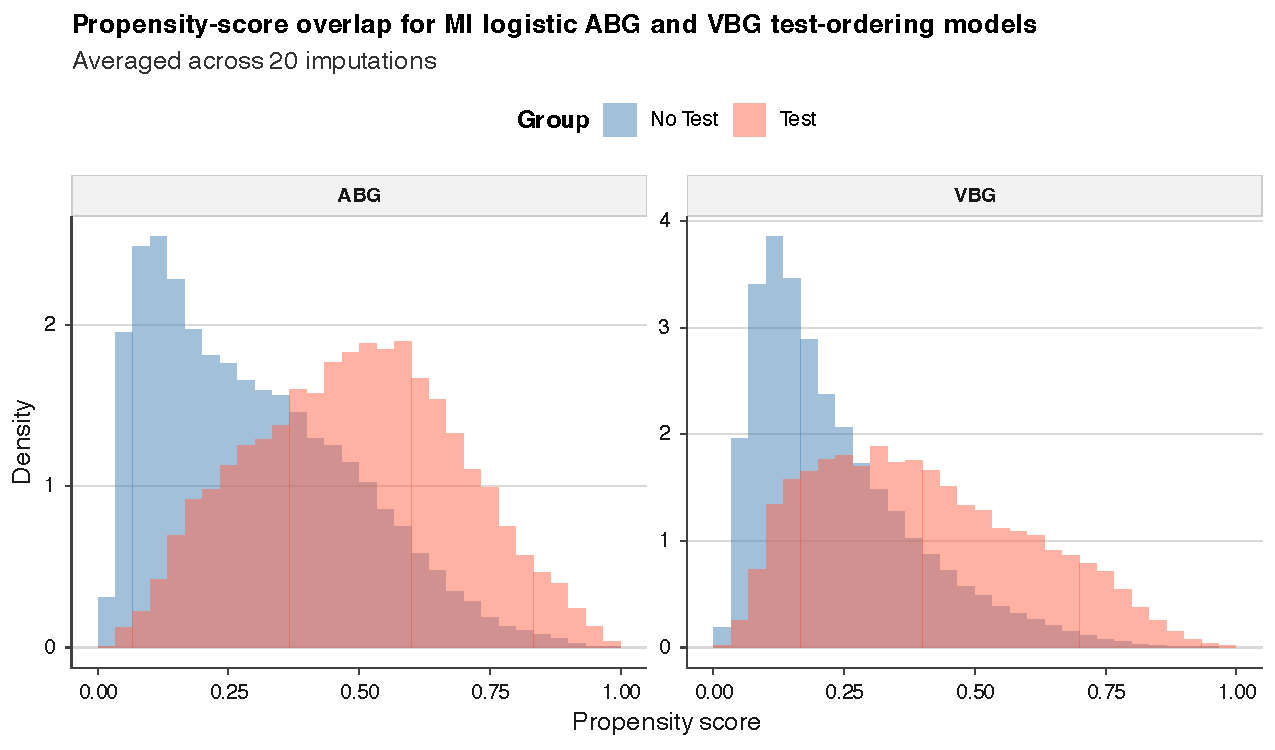
\includegraphics[width=0.88\linewidth,height=0.82\textheight,keepaspectratio]{Results/figs/figure_s2_propensity_score_overlap_mi_logistic.pdf}
\end{minipage}
\end{center}

\clearpage
\begin{center}
\begin{minipage}{\linewidth}
\centering
\small Figure S3. SHAP-style contribution summaries for MI logistic ABG and VBG test-ordering models\par
\vspace{0.5em}
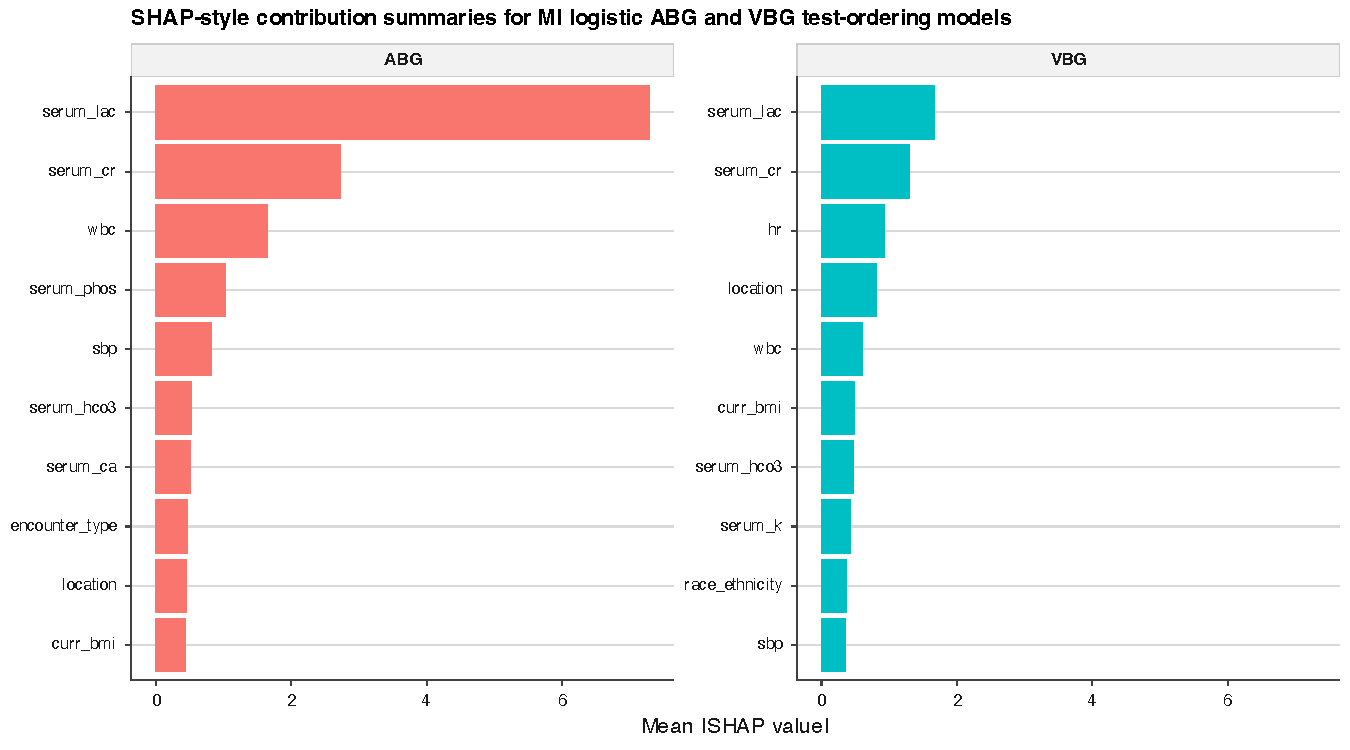
\includegraphics[width=0.88\linewidth,height=0.82\textheight,keepaspectratio]{Results/figs/figure_s3_shap_style_contributions_mi_logistic.pdf}
\end{minipage}
\end{center}

\clearpage
\begin{center}
\begin{minipage}{\linewidth}
\centering
\small Figure S4. MI-logistic IPSW-weighted categorical associations of pCO2 category with clinical outcomes by ABG and VBG\par
\vspace{0.5em}
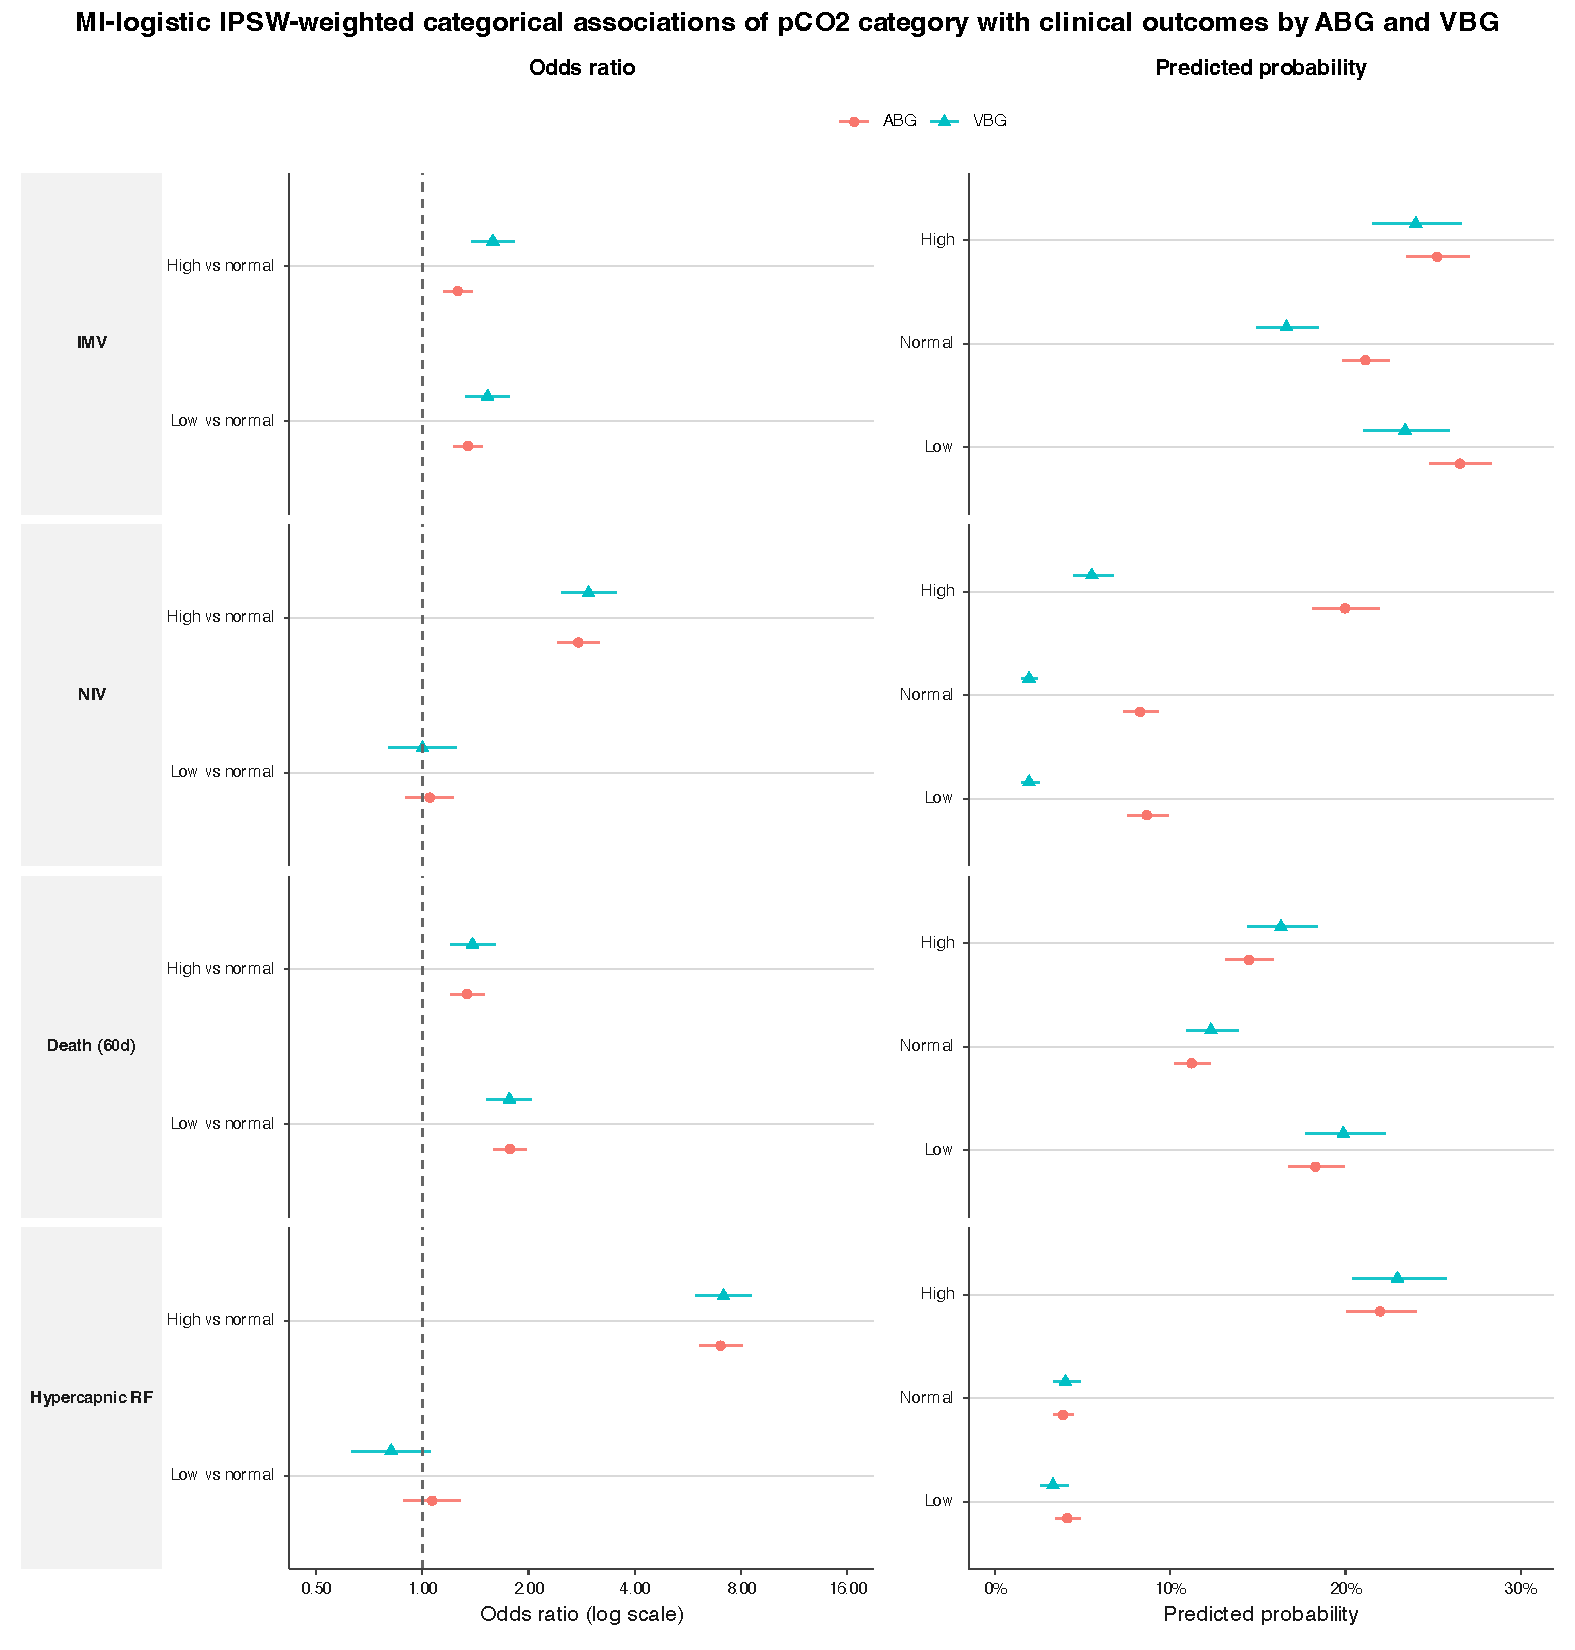
\includegraphics[width=0.88\linewidth,height=0.82\textheight,keepaspectratio]{Results/figs/figure_s4_weighted_categorical_associations_abg_vbg.pdf}
\end{minipage}
\end{center}

\clearpage
\begin{center}
\begin{minipage}{\linewidth}
\centering
\small Figure S5. Unweighted covariate-adjusted spline associations of pCO2 with clinical outcomes by ABG and VBG\par
\vspace{0.5em}
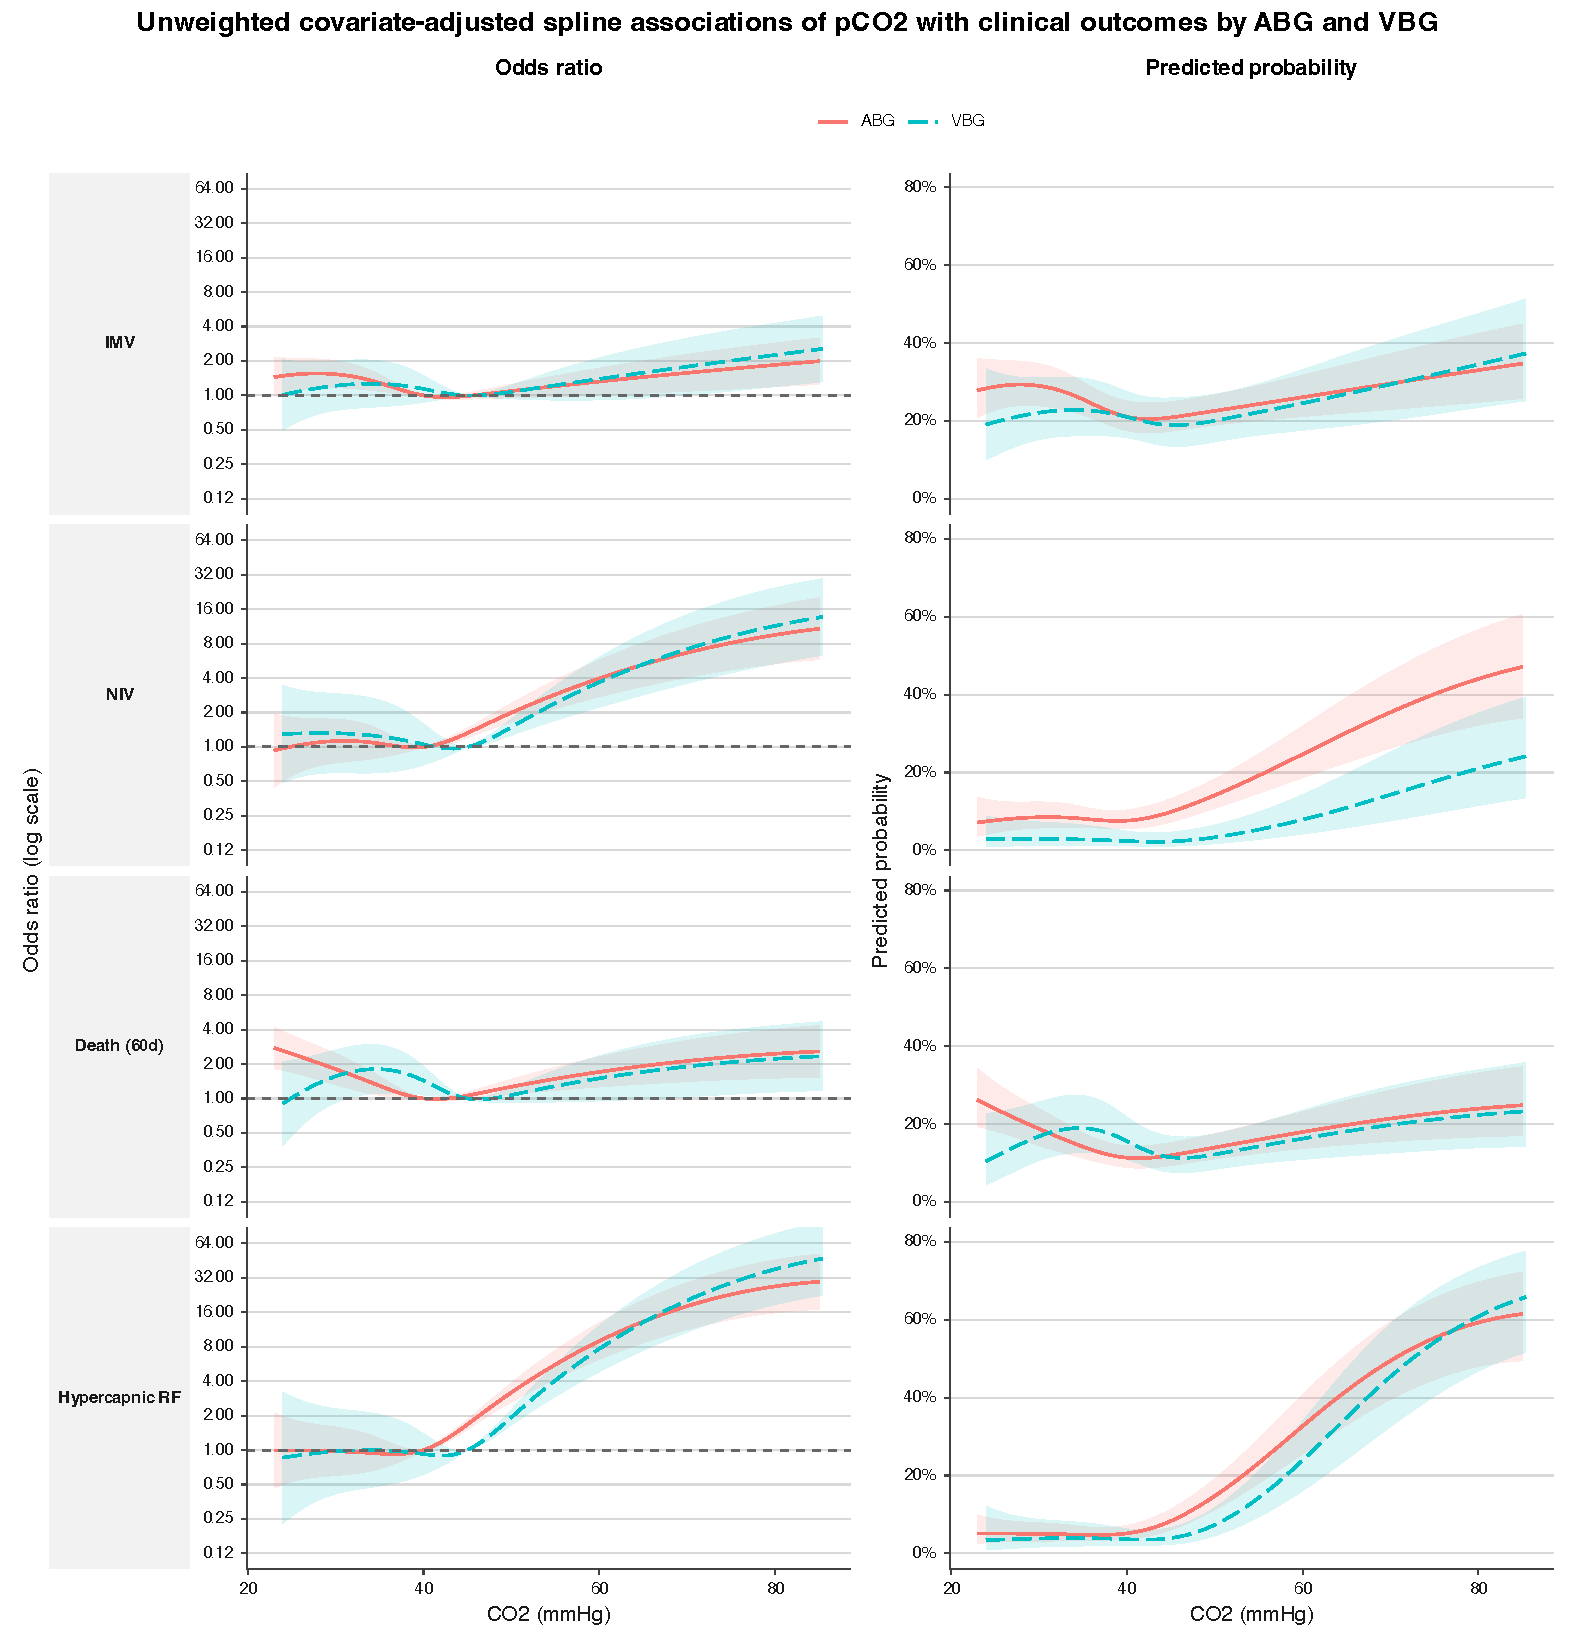
\includegraphics[width=0.88\linewidth,height=0.82\textheight,keepaspectratio]{Results/figs/figure_s5_unweighted_adjusted_spline_abg_vbg.pdf}
\end{minipage}
\end{center}

\clearpage

\begin{landscape}

\begin{center}\textbf{Table S2. Crude associations of pCO2 category with clinical outcomes by ABG and VBG}\end{center}

\begin{table}[!h]
\centering\begingroup\fontsize{6}{8}\selectfont

\resizebox{\ifdim\width>\linewidth\linewidth\else\width\fi}{!}{
\begin{tabular}{lllrrr}
\toprule
group & outcome & contrast & OR & LCL & UCL\\
\midrule
ABG & IMV & Low vs normal & 1.34 & 1.31 & 1.38\\
ABG & IMV & High vs normal & 1.24 & 1.21 & 1.27\\
ABG & NIV & Low vs normal & 1.01 & 0.97 & 1.05\\
ABG & NIV & High vs normal & 2.42 & 2.34 & 2.50\\
ABG & Death (60d) & Low vs normal & 1.90 & 1.85 & 1.95\\
\addlinespace
ABG & Death (60d) & High vs normal & 1.47 & 1.42 & 1.51\\
ABG & Hypercapnic RF & Low vs normal & 0.92 & 0.87 & 0.97\\
ABG & Hypercapnic RF & High vs normal & 5.82 & 5.62 & 6.03\\
VBG & IMV & Low vs normal & 1.48 & 1.43 & 1.54\\
VBG & IMV & High vs normal & 1.67 & 1.61 & 1.73\\
\addlinespace
VBG & NIV & Low vs normal & 1.18 & 1.12 & 1.25\\
VBG & NIV & High vs normal & 2.89 & 2.76 & 3.03\\
VBG & Death (60d) & Low vs normal & 1.78 & 1.71 & 1.84\\
VBG & Death (60d) & High vs normal & 1.61 & 1.55 & 1.67\\
VBG & Hypercapnic RF & Low vs normal & 0.98 & 0.92 & 1.04\\
\addlinespace
VBG & Hypercapnic RF & High vs normal & 7.67 & 7.33 & 8.03\\
\bottomrule
\end{tabular}}
\endgroup{}
\end{table}

\begin{table}[!h]
\centering\begingroup\fontsize{6}{8}\selectfont

\resizebox{\ifdim\width>\linewidth\linewidth\else\width\fi}{!}{
\begin{tabular}{l}
\toprule
OR (95\% CI)\\
\midrule
1.34 (1.31, 1.38)\\
1.24 (1.21, 1.27)\\
1.01 (0.97, 1.05)\\
2.42 (2.34, 2.50)\\
1.90 (1.85, 1.95)\\
\addlinespace
1.47 (1.42, 1.51)\\
0.92 (0.87, 0.97)\\
5.82 (5.62, 6.03)\\
1.48 (1.43, 1.54)\\
1.67 (1.61, 1.73)\\
\addlinespace
1.18 (1.12, 1.25)\\
2.89 (2.76, 3.03)\\
1.78 (1.71, 1.84)\\
1.61 (1.55, 1.67)\\
0.98 (0.92, 1.04)\\
\addlinespace
7.67 (7.33, 8.03)\\
\bottomrule
\end{tabular}}
\endgroup{}
\end{table}

\end{landscape}

\clearpage

\begin{landscape}

\begin{center}\textbf{Table S3. GBM IPSW-weighted associations of pCO2 category with clinical outcomes by ABG and VBG}\end{center}

\begin{table}[!h]
\centering\begingroup\fontsize{6}{8}\selectfont

\resizebox{\ifdim\width>\linewidth\linewidth\else\width\fi}{!}{
\begin{tabular}{lllrrr}
\toprule
group & outcome & contrast & OR & LCL & UCL\\
\midrule
ABG & IMV & Low vs normal & 1.36 & 1.32 & 1.40\\
ABG & IMV & High vs normal & 1.30 & 1.26 & 1.33\\
ABG & NIV & Low vs normal & 0.99 & 0.95 & 1.04\\
ABG & NIV & High vs normal & 2.68 & 2.57 & 2.79\\
ABG & Death (60d) & Low vs normal & 1.93 & 1.87 & 2.00\\
\addlinespace
ABG & Death (60d) & High vs normal & 1.45 & 1.40 & 1.50\\
ABG & Hypercapnic RF & Low vs normal & 0.94 & 0.89 & 0.99\\
ABG & Hypercapnic RF & High vs normal & 6.59 & 6.33 & 6.86\\
VBG & IMV & Low vs normal & 1.31 & 1.25 & 1.36\\
VBG & IMV & High vs normal & 1.55 & 1.49 & 1.61\\
\addlinespace
VBG & NIV & Low vs normal & 1.01 & 0.95 & 1.08\\
VBG & NIV & High vs normal & 2.91 & 2.76 & 3.06\\
VBG & Death (60d) & Low vs normal & 1.77 & 1.70 & 1.85\\
VBG & Death (60d) & High vs normal & 1.46 & 1.40 & 1.52\\
VBG & Hypercapnic RF & Low vs normal & 0.86 & 0.80 & 0.93\\
\addlinespace
VBG & Hypercapnic RF & High vs normal & 8.21 & 7.79 & 8.65\\
\bottomrule
\end{tabular}}
\endgroup{}
\end{table}

\begin{table}[!h]
\centering\begingroup\fontsize{6}{8}\selectfont

\resizebox{\ifdim\width>\linewidth\linewidth\else\width\fi}{!}{
\begin{tabular}{l}
\toprule
OR (95\% CI)\\
\midrule
1.36 (1.32, 1.40)\\
1.30 (1.26, 1.33)\\
0.99 (0.95, 1.04)\\
2.68 (2.57, 2.79)\\
1.93 (1.87, 2.00)\\
\addlinespace
1.45 (1.40, 1.50)\\
0.94 (0.89, 0.99)\\
6.59 (6.33, 6.86)\\
1.31 (1.25, 1.36)\\
1.55 (1.49, 1.61)\\
\addlinespace
1.01 (0.95, 1.08)\\
2.91 (2.76, 3.06)\\
1.77 (1.70, 1.85)\\
1.46 (1.40, 1.52)\\
0.86 (0.80, 0.93)\\
\addlinespace
8.21 (7.79, 8.65)\\
\bottomrule
\end{tabular}}
\endgroup{}
\end{table}

\end{landscape}

\clearpage
\begin{center}
\begin{minipage}{\linewidth}
\centering
\small Figure S6. Covariate balance after gradient-boosted propensity weighting for ABG and VBG test-ordering models\par
\vspace{0.5em}
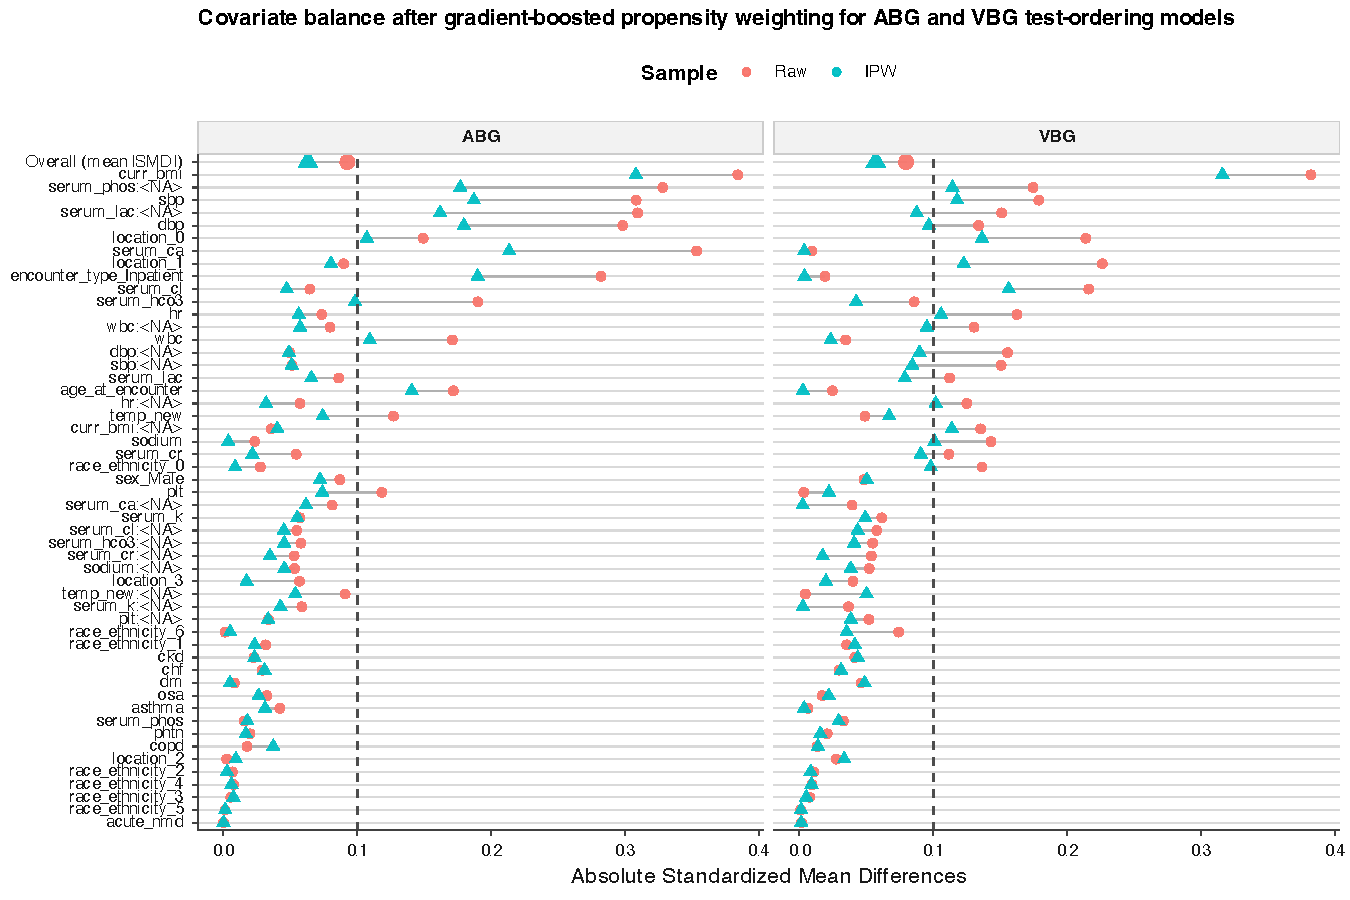
\includegraphics[width=0.88\linewidth,height=0.82\textheight,keepaspectratio]{Results/figs/figure_s6_covariate_balance_gbm_weighting.pdf}
\end{minipage}
\end{center}

\clearpage
\begin{center}
\begin{minipage}{\linewidth}
\centering
\small Figure S7. Propensity-score overlap for gradient-boosted ABG and VBG test-ordering models\par
\vspace{0.5em}
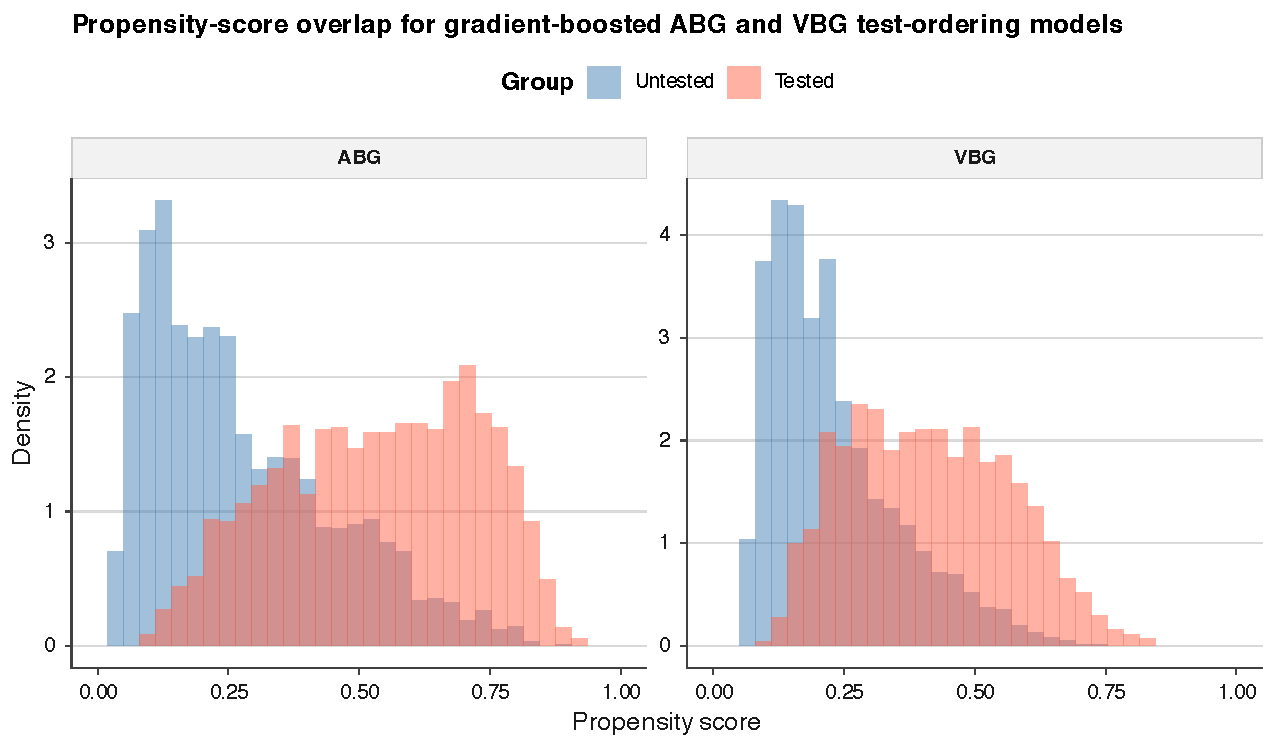
\includegraphics[width=0.88\linewidth,height=0.82\textheight,keepaspectratio]{Results/figs/figure_s7_propensity_score_overlap_gbm.pdf}
\end{minipage}
\end{center}

\clearpage
\begin{center}
\begin{minipage}{\linewidth}
\centering
\small Figure S8. SHAP-style contribution summaries for gradient-boosted ABG and VBG test-ordering models\par
\vspace{0.5em}
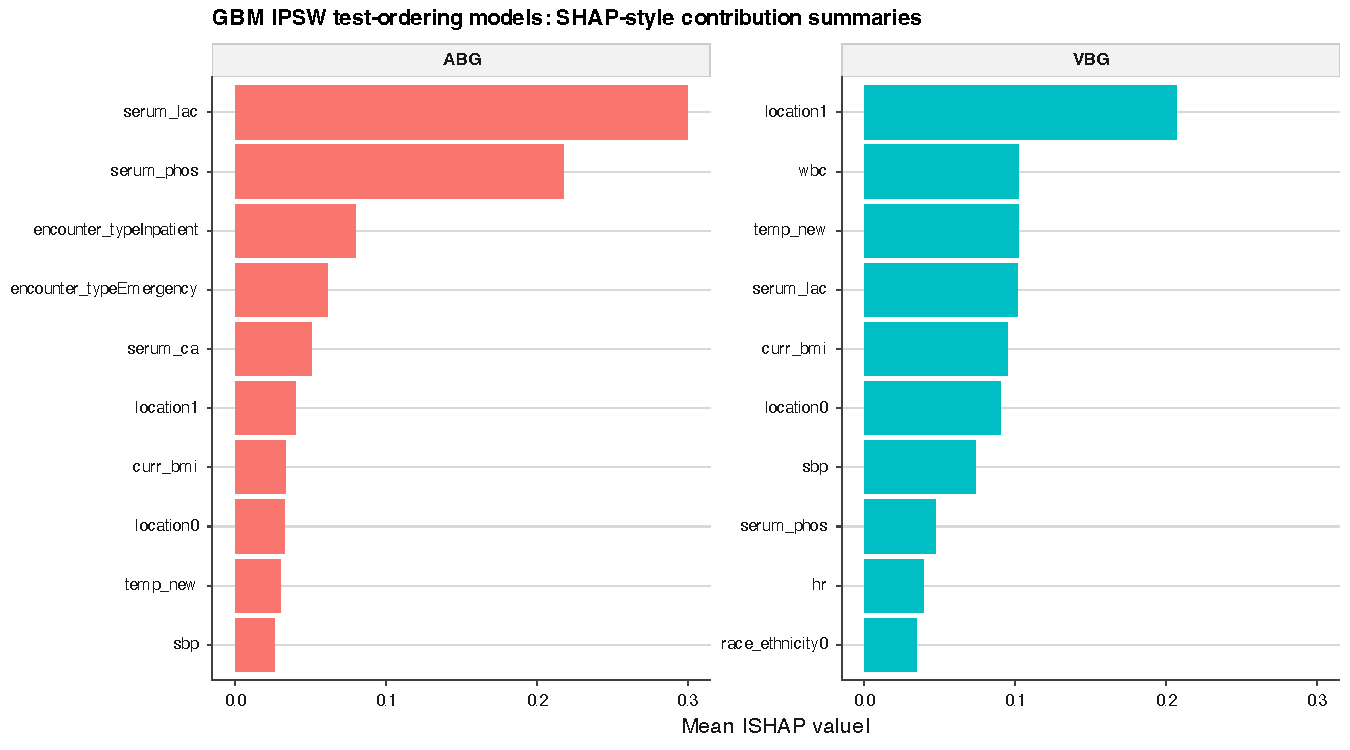
\includegraphics[width=0.88\linewidth,height=0.82\textheight,keepaspectratio]{Results/figs/figure_s8_shap_style_contributions_gbm.pdf}
\end{minipage}
\end{center}\begin{center}\textbf{Artifact check summary}\end{center}

\begin{table}[!h]
\centering\begingroup\fontsize{7}{9}\selectfont

\resizebox{\ifdim\width>\linewidth\linewidth\else\width\fi}{!}{
\begin{tabular}{lllr}
\toprule
check\_status & severity & allowed\_missing & n\_rows\\
\midrule
present & none & FALSE & 56\\
external\_manual\_declared & info & TRUE & 1\\
suppressed\_draft\_only & none & TRUE & 1\\
\bottomrule
\end{tabular}}
\endgroup{}
\end{table}\begin{landscape}

\begin{center}\textbf{Diagnostics audit summary}\end{center}

\begin{table}[!h]
\centering\begingroup\fontsize{6}{8}\selectfont

\resizebox{\ifdim\width>\linewidth\linewidth\else\width\fi}{!}{
\begin{tabular}{llllll}
\toprule
component & metric & status & severity & value & note\\
\midrule
Audit & overall\_status & fail & high & FAIL & Overall diagnostics audit status derived from the highest-severity unresolved issue.\\
Outcome & separation\_flags\_total & fail & high & 328 & Separation or near-separation can bias ORs and confidence intervals.\\
Inventory & expected\_artifacts\_missing & pass & none & 0 & Count of expected diagnostics artifacts missing from Results/.\\
MI & smoke\_test\_failed & pass & none & FALSE & Smoke test failure indicates the MI execution path is unstable.\\
MI & chain\_diagnostics\_issue & pass & none & FALSE & numeric\_names=FALSE; drift\_tail\_na\_frac=0.000\\
\addlinespace
Balance & abg\_max\_abs\_smd & pass & none & 0.091 & ABG target balance threshold is 0.10.\\
Balance & vbg\_max\_abs\_smd & pass & none & 0.042 & VBG target balance threshold is 0.10.\\
Plotting & plot\_drop\_log\_present & pass & none & TRUE & Plot drop logging should exist even if no rows are present.\\
\bottomrule
\end{tabular}}
\endgroup{}
\end{table}

\end{landscape}\begin{landscape}

\begin{center}\textbf{Diagnostics audit issues}\end{center}

\begin{table}[!h]
\centering\begingroup\fontsize{6}{8}\selectfont

\resizebox{\ifdim\width>\linewidth\linewidth\else\width\fi}{!}{
\begin{tabular}{llllll}
\toprule
severity & component & evidence\_file & evidence\_snippet & why\_it\_matters & recommended\_fix\\
\midrule
high & Outcome & Results/model\_fit\_diagnostics.csv & sep\_flag TRUE for 328 / 2612 fits & High rate of separation/near-separation can bias ORs and CIs. & Inspect flagged outcomes; consider penalized fits or check data sparsity.\\
\bottomrule
\end{tabular}}
\endgroup{}
\end{table}

\begin{table}[!h]
\centering\begingroup\fontsize{6}{8}\selectfont

\resizebox{\ifdim\width>\linewidth\linewidth\else\width\fi}{!}{
\begin{tabular}{ll}
\toprule
run\_id & run\_ts\\
\midrule
20260419\_112645 & 2026-04-19 11:26:45.267227\\
\bottomrule
\end{tabular}}
\endgroup{}
\end{table}

\end{landscape}

Software: R 4.5.3 ; key packages: mice, WeightIt, cobalt, survey, rms.




\end{document}
